\documentclass[english, 11pt]{article}
\usepackage{notes}
\usetikzlibrary{decorations.pathmorphing}
%\renewcommand{\sfdefault}{cmss}
%\renewcommand{\familydefault}{\sfdefault}

\newcommand{\thiscoursecode}{MATH 239}
\newcommand{\thiscoursename}{Introduction to Combinatorics}
\newcommand{\thisprof}{Dr. Kevin Purbhoo}
\newcommand{\me}{Liam Horne}
\newcommand{\thisterm}{Fall 2013}
\newcommand{\website}{LIHORNE.COM}

% Headers
\chead{\thiscoursename}
\lhead{\thisterm}


%%%%% TITLE %%%%%
\newcommand{\notefront} {
\pagenumbering{roman}
\begin{center}

{\ttfamily \url{\website}} {\small}

\textbf{\Huge{\noun{\thiscoursecode}}}{\Huge \par}

{\Large{\noun{\thiscoursename}}}\\ \vspace{0.1in}

\vspace{0in}
\includegraphics[scale=0.5]{logo.png}

  %\includegraphics[scale=0.1]{shield.png} \\
  {\noun \thisprof} \ $\bullet$ \ {\noun \thisterm} \ $\bullet$ \ {\noun {University of Waterloo}} \\

  \end{center}
  }

%   ooooo      ooo   .oooooo.   ooooooooooooo oooooooooooo  .oooooo..o
%   `888b.     `8'  d8P'  `Y8b  8'   888   `8 `888'     `8 d8P'    `Y8
%    8 `88b.    8  888      888      888       888         Y88bo.
%    8   `88b.  8  888      888      888       888oooo8     `"Y8888o.
%    8     `88b.8  888      888      888       888    "         `"Y88b
%    8       `888  `88b    d88'      888       888       o oo     .d8P
%   o8o        `8   `Y8bood8P'      o888o     o888ooooood8 8""88888P'


% \DeclareMathVersion{sans}
% \SetSymbolFont{operators}{sans}{OT1}{cmbr}{m}{n}
% \SetSymbolFont{letters}{sans}{OML}{cmbrm}{m}{it}
% \SetSymbolFont{symbols}{sans}{OMS}{cmbrs}{m}{n}
% \SetMathAlphabet{\mathit}{sans}{OT1}{cmbr}{m}{sl}
% \SetMathAlphabet{\mathbf}{sans}{OT1}{cmbr}{bx}{n}
% \SetMathAlphabet{\mathtt}{sans}{OT1}{cmtl}{m}{n}
% \SetSymbolFont{largesymbols}{sans}{OMX}{iwona}{m}{n}
\begin{document}
% \renewcommand\familydefault{\sfdefault}

% \sffamily\mathversion{sans}
  % Notes front
  \notefront
  % Table of Contents and List of Figures
  \tocandfigures
  % Abstract
  \doabstract{These notes are intended as a resource for myself; past, present, or future students of this course, and anyone interested in the material. The goal is to provide an end-to-end resource that covers all material discussed in the course displayed in an organized manner. If you spot any errors or would like to contribute, please contact me directly.}

  \section{Combinatorial Analysis}


  \subsection{Binomial Coefficients}

  \begin{exmp}
    Consider the subsets of a three element set $\{1,2,3\}$. We have,
    \[ \underbrace{\emptyset}_{0\mbox{ elements}}, \underbrace{\{1\}, \{2\}, \{3\}}_{1\mbox{ element}}, \underbrace{\{1, 2\}, \{1,3\}, \{2,3\}}_{2\mbox{ elements}},  \underbrace{\{1,2,3\}}_{3\mbox{ elements}} \]

  \end{exmp}


  \begin{defn}
    $n\choose k$ is the number of $k$-element subsebts of $\{1,2,3,\cdots,n\}$ read "$n$ choose $k$", for example ${3 \choose 2 }= 3$.
  \end{defn}

  \begin{exmp}
    Consider binary strings of length 3.

    \[ \underbrace{000}_{0\times 1s}, \underbrace{001, 010, 100}_{1\times 1}, \underbrace{011, 101, 110}_{2\times 1's},  \underbrace{111}_{3\times 1s}  \]

    This is essentially the same as our last example.
  \end{exmp}

  \begin{defn}
    $n \choose k$ is the number of binary strings of length $n$ with exactly $k$ digits of "1".
  \end{defn}

  \begin{defn}
    \[ {n \choose k} := \frac{n(n-1)(n-2)\cdots(n-k+1)}{k(k-1)(k-2)\cdots1} = \frac{n!}{(n-k)!k!}\]
    This can be thought of as the numerator being the number of ways to list $k$ different elements of a set of $n$ elements and the denominator being the number of ways these lists can be ordered.
  \end{defn}

  \begin{thrm}
    \[ {n \choose k} = {n \choose n - k} \]
  \end{thrm}

  \begin{proof}[Algebraic Proof]
    \begin{align*}
      LHS & = {n \choose k} = \frac{n!}{(n-k)!k!} \\
      RHS & = {n \choose n - k} = \frac{n!}{(n-(n-k))!(n-k)!} = \frac{n!}{k!(n-k)!}
    \end{align*}
  \end{proof}

  \begin{defn}
    Let $S$ be a set. Then $|S_k|$ is defined to be the \textbf{cardinality} of $S$. That is, it is the number of elements in $S$.
  \end{defn}

  \begin{proof}[Combinatorial Proof]
    Let $S_k$ be the set of all $k$-element subsets of $\{1,2,\cdots,n\}$. Then, according to Definition 1,
    \begin{align*}
      LHS = {n \choose k} = |S_k| \\
      RHS = {n \choose n - k} = |S_{n-k}|
    \end{align*}
    To do this, we need to find a bijection between $S_k$ and $S_{n-k}$. We need to define the complement.

    \begin{defn}
      If $A \subseteq \{ 1, \cdots, n \}$, let $A^{\complement} = \{ i \in \{ 1, \cdots, n \} | i \not \in A \}$
    \end{defn}

    Note firstly that if $A \in S_k$ then $A ^{\complement} \in S_{n-k}$ and the map $S_k \rightarrow S_{n-k}$ is a bijection. \\
    This shows that $|S_k| = |S_{n-k}|$ and therefore
    $${n \choose k} = {n \choose n -k}$$
  \end{proof}

  In this example I can describe a $k$-element subset of $\{1,\cdots,n\}$ in two ways. First, what elements are in it, and what elements are not in it.

  \begin{defn}
    If $A_1, \cdots, A_k$ are sets, we say that they are \textbf{pairwise disjoint} if $A_i \cap A_j = \emptyset$ for $i \not = j$. If this is the case,
    \[ \left|\bigcup_{i=1}^k A_i\right| = \sum_{i=1}^k |A_i| \]
  \end{defn}

  \begin{exmp}
    Prove that
    $${n + k \choose n} = \sum_{i=0}^k {n+i-1\choose n-1}$$
  \end{exmp}

  \begin{proof}
    Let $\mathscr{S}  =$ set of $n$-element subsets of $\{ 1,2,\cdots,n+k \}$. Then,
    \[ \mathscr{S} = {n+k\choose n} \]
    Let $\mathscr{S}_i$ be the set of $n$-element subsets of $\{1,\cdots,n+k\}$ whose largest element is $n+i, i = 0,1,2,\cdots,k$. Note that $\mathscr{S} _0, \cdots, \mathscr{S} _k$ are pairwise disjoint. Then,
    \[ |\mathscr{S} | = \sum_{i=0}^k |\mathscr{S}_i| \]
    Now, if $A \in \mathscr{S}$ then $n + i \in A$ and $A \setminus \{ n + i \}$ is an $(n-1)$-element subset of $\{1,\cdots,n+i-1\}$. Then,
    $$|\mathscr{S} _i| = {n+i-1\choose n-1}$$
  \end{proof}

  \begin{defn}[cartesian product]\label{cartesian product}
    Let $A$ and $B$ be sets, then the \textbf{Cartesian Product} of $A$ and $B$ is
    \[ A \times B = \{ (a,b) | a \in A, b \in B \} \]
    and then
    \[ |A \times B| = |A|\cdot|B| \]
  \end{defn}

  \begin{exmp}
    Prove that
    \[ {m + n \choose k} = \sum_{i=0}^k {m \choose i} {n \choose k - i} \]
  \end{exmp}

  \begin{proof}
  Let $M = \{ 1,\cdots, m\}$ and $N = \{ m+1, \cdots, m + n\}$, then $M\cup N = \{ 1, \cdots, m+n\}$. If $X$ is a set, let $S_k(X)$ denote the set of $k$-element subsets of $X$.
    \begin{align*}
      LHS & = {m + n \choose k} \\
          & = |S_k(M\cup N)|
    \end{align*}
  We break it down according to how many elements are from $M$.
  So,
  \begin{align*}
      RHS & = \left| \bigcup_{i=0}^k S_i(M) \times S_{k-i}(N) \right|
    \end{align*}
  \end{proof}

Proof left as an exercise to the reader. \\

Consider $f(y_1,y_2,y_3) = (1+y_1)(1+y_2)(1+y_3)$, multiplying together we get
\begin{align*}
  (1+y_1)(1+y_2)(1+y_3) & = (1+y_2+y_1+y_1y_2)(1+y_3) \\
  & = 1 + y_2 + y_2 + y_3 + y_1y_2 + y_1y_3 + y_2y_3 + y_1y_2y_3
\end{align*}
Note that the subsets of $\{ 1, 2, 3 \}$ are in a way built into this expansion. Now we consider $y_1=y_2=y_3=x$, then
\[ f(x,x,x) = (1+x)^3 = \ub{1} + \ub{3}x + \ub3x^2 + \ub1x^3 \]
Hence we can restate $(1+x)^3$ as
\[ (1+x)^3 = \comb{3}{0}x^0 + \comb{3}{1}x^2 + \comb{3}{2}x^2 + \comb{3}{3}x^3 \]
Generalizing this reasoning lets us define something new.

\begin{defn}[binomial theorem]\label{binomialtheorem}
  The \textbf{Binomial Theorem} states that for $n \in \N$
  \[ (1+x)^n = \sum_{k=0}^n \comb{n}{k}x^k \]
\end{defn}

\begin{exmp}
  Prove that
  \[ \comb{n}{k} = \comb{n}{n-k} \]
\end{exmp}
\begin{proof}
 First consider the fact that $(1+x) = x\left(1+\f{1}{x}\right)$, then
 \begin{align*}
   (1+x)^n & = \sum_{j=0}^n \comb{n}{j} x^j \\
   \implies \left(x\left(1 + \f{1}{x}\right)\right)^n & = x^n\left(1+\f{1}{x}\right)^n \\
   & = x^n \left[ \sum_{k=0}^n \comb{n}{k} \left(\f{1}{x}\right)^k\right] \\
   & =  \sum_{k=0}^n x^n \comb{n}{k} \left(\f{1}{x}\right)^k \\
   & = \sum_{k=0}^n \comb{n}{k} x^{n-k}
 \end{align*}
 Now, we substitute $j = n - k$, thus $k = n - j$. So,
\[ \sum_{k=0}^n \comb{n}{k} x^{n-k} = \sum_{j=0}^n \comb{n}{n-j}x^j \]
Therefore
\[ (1+x)^n = \sum_{j=0}^n \comb{n}{j} x^j = \sum_{j=0}^n \comb{n}{n-j} x^j\]
\end{proof}

\begin{exmp}
  Prove that
  \[ \comb{m+n}{k} = \sum_{i=0}^k \comb{m}{i} \comb{n}{k-i} \]
  The hint is that $(1+x)^{m+n} = (1+x)^m(1+x)^n$. So,
  \[ LHS = (1+x)^{m+n} = \sum_{k = 0}^{m+n} \comb{m+n}{k}x^k \]
  \[ RHS = (1+x)^m(1+x)^n = \left[\sum_{i=0}^m\comb{m}{i}x^i\right]\left[\sum_{j=0}^n\comb{n}{j}x^j\right] \]
  Expanding the right hand side we get,
  \begin{align*}
    \left[\sum_{i=0}^m\comb{m}{i}x^i\right]\left[\sum_{j=0}^n\comb{n}{j}x^j\right] & = \sum_{j=0}^n\sum_{i=0}^m \comb{m}{i} \comb{n}{j}x^{i+j}
  \end{align*}
  Now we substitute $k = i + j$ to eliminate $j$, hence $j = k - i$,
  \[ \sum_{j=0}^{n}\sum_{i=0}^{\min(k,m)} \comb{m}{i}x^i \comb{n}{j}x^j  = \sum_{k=0}^{m+n}\sum_{j=0}^{k} \comb{m}{i}x^i \comb{n}{k-i}x^{k} \]
  Note that
  \[ (1+x)^{m+n} = \sum_{k=0}^{m+n} \comb{m+n}{k} x^k = \sum_{k=0}^{m+n} \sum_{i=0}^{\min(k,m)} \comb{m}{i}\comb{n}{k-i}x^k \]
  We conclude that
  \[ \comb{m+n}{k} = \sum_{i=0}^{\min(k,m)}\comb{m}{i}\comb{n}{k-i} \]
  So finally note that
  \[ \sum_{i=0}^{\min(k,m)} \comb{m}{i} \comb{n}{k-i} = \sum_{i=0}{k}\comb{m}{i}\comb{n}{k-i} \]
  Because additional $i$-values on RHS are $i > m$ and $\comb{m}{i} = 0$ for these. Note since $\comb{n}{k} = 0$, for $k > n$ we sometimes write the binomial theorem as
  \[ (1+x)^n = \sum_{k=0}^{\infty}\comb{n}{k}x^k \]
\end{exmp}

  There is a third $\sum$ notation trick, that is turning a sum into a sum of sums or split of terms. For example
  \[ \sum_{k=0}^n a_k = a_0 + \sum_{k=1}^n a_k = a_0 + a_1 + \sum_{k=2}^n a_k = \cdots \]

  \subsection{Generating Functions}

  The idea of a generating function is that we can take enumeration word problems that are either hard or easy, and translate them into the language of generating functions and using the tools of generating functions to turn a hard problem to an easy problem at which point they are again translatable to an easy word problem. \\

  The idea is to phrase all problems in the same way.

  \begin{center}
    How many $x$'s are there with property $y$?
  \end{center}

  \begin{defn}[weight function]\label{weight function}
    Let $S$ be a set of objects. A \textbf{weight function} on $S$ is a function $w:S\rightarrow \N = \{0,1,2,3,\ldots\}$ which assigns to each $\sigma \in S$ a non-negative integer $w(\sigma)$ called the \textbf{weight} of $\sigma$.
  \end{defn}

  \begin{exmp}
    Take $S =$ binary strings of length 4. Also, the \nameref{weight function} $w(\sigma) =$ number of 1's in $\sigma$. For example, $w(0110) = 2$.
  \end{exmp}

  In this setup, the general counting problem is: how many elements of $S$ are there of weight $n$?

   \begin{defn}[generating function]\label{generating function}
     Let $w$ be a \nameref{weight function} on a set $S$. The \textbf{generating function} for $S$ with respect to $w$ is
     \[ \Phi_S(x) = \sum_{\sigma \in S} x^{w(\sigma)} \]
   \end{defn}

   \begin{exmp}
     Consider the same set $S$ of binary strings of length 4, where $w(\sigma)$ is the number of 1's in $\sigma$. Find the generating function $\Phi_S(x)$. \\
     To solve this problem, we create a table:
     \begin{tabular}{c | c | c || c | c | c }
       $\sigma$ & $w(\sigma)$ & $x^{w(\sigma)}$ & $\sigma$ & $w(\sigma)$ & $x^{w(\sigma)}$ \\
       \hline
       0000 & 0 & 1 & 1000 & 1 & x \\
       0001 & 1 & x & 1001 & 2 & $x^2$ \\
       0010 & 1 & x & 1010 & 2 & $x^2$ \\
       0100 & 1 & x & 1100 & 2 & $x^2$ \\
       0011 & 2 & $x^2$ & 1011 & 3 & $x^3$ \\
       0101 & 2 & $x^2$ & 1101 & 3 & $x^3$ \\
       0110 & 2 & $x^2$ & 1110 & 3 & $x^3$ \\
       0111 & 3 & $x^3$ & 1111 & 4 & $x^4$ \\
     \end{tabular}

     So,
     \[ \Phi_S(x) = 1 + x + x + x^2 + \cdots = 1 + 4x + 6x^2 + 4x^3 + x^4 \]
     We can make the following observations from this example:
     \begin{itemize}
       \item[(i)] The coefficient of $x^i$ is the number of elements of weight (see \nameref{weight function}) $i$ in $S$
       \item[(ii)] $\Phi_S(x) = (1+x)^4$
       \item[(iii)] $\Phi_S(1) = 16 = |S|$
       \item[(iv)] $\f{d\Phi_S(x)}{dx} = 4 + 12x + 12x^2 + 4x^3$ and $\f{d\Phi_S(1)}{dx} = 32 = \sum_{\sigma \in S} w(\sigma)$
     \end{itemize}
   \end{exmp}

   We can turn this into a general answer.

   \begin{thrm}
     Let $S$ be a set of objects with a weight function $w$. Let
     \[ \Phi_S(x) = \sum_{n=0}^{\infty}a_nx^n \]
     Then $a_n$ is the number of elements of $S$ having weight $n$.
   \end{thrm}


   \begin{proof}
     \begin{align*}
         \Phi_S(x) & = \sum_{\sigma \in S} x^{w(\sigma)} \\
         & = \sum_{n=0}^{\infty} \sum_{\substack{\sigma \in S \\ w(\sigma)=n}} x^{w(\sigma)} \\
         & = \sum_{n = 0}^{\infty} \sum_{\substack{\sigma \in S \\ w(\sigma)=n}} x^n \\
         & = \sum_{n=0}^{\infty} \left( \sum_{\substack{\sigma \in S \\ w(\sigma)=n}} 1\right) x^n
      \end{align*}
      Since $\Phi_S(x) = \sum_{n=0}^{\infty}a_nx^n = \sum_{n = 0}^{\infty} \left( \sum_{\substack{\sigma \in S \\ w(\sigma)=n}} 1\right) x^n$ \\
      Therefore, $a_n = \sum_{\substack{\sigma \in S \\ w(\sigma)=n}} 1$ which is the number of elements of $S$ having weight $n$.
   \end{proof}

   \begin{notation}
     We call $a_n$ the coefficient of $x^n$ in $\Phi_S(x)$ and write this as
     \[ [x^n]\Phi_S(x) \]
     That is, the answer to our general question is always $[x^n]\Phi_S(x)$.
   \end{notation}

   \begin{thrm}
     Let $S$ be a finite set with weight function $w$. Let $\Phi_S(x)$ be the generating function. Then,
     \begin{itemize}
       \item[(i)] $\displaystyle\Phi_S(1) = |S|$
       \item[(ii)] $\Phi_S'(1) = \displaystyle\sum_{\sigma \in S} w(\sigma) =$ "sum of the weights of elements in $S$"
       \item[(iii)] $\displaystyle\f{\Phi_S'(1)}{\Phi_S(1)} = \f{\sum_{\sigma \in S} w(\sigma)}{|S|} =$ "average of weights"
     \end{itemize}
   \end{thrm}

   See the course notes for the proof.

   \begin{exmp}
     Let $S$ be the set of all binary strings (infinite set). For $\sigma \in S$, define weight function $w(\sigma)$ = "length of $\sigma$" \\

     Let $S = \{ \epsilon, 0,1,00,01,10,11,000,\ldots \}$ with $\epsilon$ denoting the string of length 0. In this context, our question is how many \ubt{binary strings}{elements of $S$} are there of weight $n$. The answer from intuition is $2^n$. So we conclude that
     \[ [x^n]\Phi_S(x) = 2^n \]
     and
     \[ \Phi_S(x) = \sum_{n=0}^{\infty} (2x)^n \]
     where these statements are equivalent.
     \begin{note}
       In general,
     \[ [x^n]\Phi_S(x) = a_n \iff \Phi_S(x) = \sum_{n=0}^{\infty} a_nx^n \]
     \end{note}
     Also, we notice that our sum is a geometric series, so we can expand
     \[ \Phi_S(x) = \sum_{n=0}^{\infty} (2x)^n = 1 + (2x) + (2x)^2 + \cdots = \f{1}{1-2x}  \]
     We can question this result; does it make sense?
     \begin{itemize}
       \item[A1.] \textbf{Yes}, if $-\f{1}{2} < x < \f{1}{2}$.
       \item[A2.] \textbf{Yes}, in the context of formal power series.
     \end{itemize}
   \end{exmp}

   \subsection{Formal Power Series}

   The idea is to think about power series in terms of the operations you are \textbf{allowed} to perform on them. We want to get rid of the concept of radius of convergence.

   \begin{defn}[formal power series]\label{power series}
     A formal power series is a power series such as
     \[ A(x) = \sum_{n=0}^{\infty} a_nx^n \]
     but $A(x)$ should not be thought of as a function. \textit{We disallow the ability to plug in numbers} (some exceptions to be discussed). The following are the allowed operations:
     \begin{itemize}
       \item Coefficient Extraction: $[x^n]A(x) = a_n$.
       \item Arithematic Operations: Consider $A(x) = \sum_{n=0}^{\infty}, B(x) = \sum_{n=0}^{\infty}$, then
       \begin{itemize}
         \item[i.] $\displaystyle A(x) + B(x) =  \sum_{n=0}^{\infty} (a_n + b_n)x^n$
         \item[ii.] $\displaystyle A(x) - B(x) =  \sum_{n=0}^{\infty} (a_n - b_n)x^n$
         \item[iii.] $\displaystyle cA(x) =  \sum_{n=0}^{\infty} (ca_n)x^n$
         \item[iv.] $\displaystyle A(x)B(x) = \left( \sum_{j=0}^{\infty} a_ix^j\right)\left(  \sum_{k=0}^{\infty} b_kx^k \right) = \sum_{k=0}^{\infty}\sum_{j=0}^{\infty} b_ka_ix^{j+k}$, then substitute $n = j+k$ to get
         \[ A(x)B(x)= \sum_{n=0}^{\infty}\left(\sum_{j=0}^{n} a_jb_{n-j}\right)x^{n} \]
         Another way to think about this is \\
         \begin{center}
         \begin{tabular}{c || c | c | c | c}
           {} & $a_0 +$ & $a_1x +$ & $a_2x^2 +$ & $a_3x^3 + \cdots$ \\
           \hline
           \hline
           $b_0$ & $a_0b_0$ & $a_1b_0x$ & $a2b_0x^2$ & $a_3b_0x^3$ \\
           \hline
           $+b_1x$ & $a_0b_1x$ & $a_1b_1x^2$ & $a2b_1x^3$ \\
           \hline
           $+b_2x^2$ & $a_0b_2x^2$ & $a_1b_2x^3$ \\
           \hline
           $+b_3x^3$ & $a_0b_3x^3$ \\
           \hline
           $+\vdots$
         \end{tabular}
         \end{center}
       \end{itemize}
       \item Division / Inverses : If $A(x)B(x)= 1 = 1 + x + 0x^2 + 0x^3 + \cdots$ then we say $B(x)$ is the inverse of $A(x)$ and
       \[ B(x) = \f{1}{A(x)} \mbox{ \ \ \ \ or \ \ \ \ } B(x) = A(x)^{-1} \]
       This obeys the usual properties of division or inverses. Note that not every formal power series has an inverse.
        \begin{thrm}
     Let $A(x)$ be a formal power series
     \[ A(x) = \sum_{a=0}^{\infty} a_nx^n \]
     then $A(x)$ has an inverse if and only if $a_0 \not = 0$.
   \end{thrm}

   Proof in the course notes.

   \begin{exmp}
     For some problem we can take the formal power series.
     \[ A(x) = x = 0 + 1x + 0x^2 + 0x^3 + \cdots \]
     We know that $\f{1}{A(x)} = \f{1}{x}$ which is not a formal power series, so there is no inverse. Consider again $B(x)A(x) = 1$, then since $B(x)A(x) = a_0b_0 + (a_1b_0+a_0b_1)x + \cdots \implies a_0b_0 = 1$. However, $a_0 = 0$ here, so there is no inverse.
   \end{exmp}
   \item Composition / Substitution
   $A(B(x))$ doesn't always make sense, so it is allowed in two cases.
   \begin{itemize}
     \item[i.] $b_0 = 0$
     \item[ii.] $A(x)$ is a polynomial
   \end{itemize}
     \end{itemize}
   \end{defn}

  To summarize what we know of Formal Power Series; we are allowed to use operators of addition, multiplication, substraction, and scalar multiplciation. As well, we can extract coefficients, deal with inverses (sometimes), and substitutions (sometimes). We disallow plugging in numbers, limits in the traditional sense, and infinite sums of numbers. Radius of convergence is also not allowed. \\

  Recall that
  \[ \sum_{n=0}^{\infty} 2^n x^n = \f{1}{1-2x}. \]
  Interpeted in \nameref{power series} we see that $1 - 2x$ is the \nameref{power series} inverse of $\sum_{n=0}^{\infty} 2^nx^n$ which means that
  \[ (1-2x)\left( \sum_{n=0}^{\infty} 2^nx^n\right) = 1 = 1 + 0x + 0x^2 + 0x^3 + \cdots \]
  Check \\
   \begin{center}
         \begin{tabular}{c || c | c | c | c}
           {} & $1 +$ & $2x +$ & $4x^2 +$ & $8x^3 + \cdots$ \\
           \hline
           \hline
           $1$ & $1$ & $2x$ & $4x^2$ & $8x^3$ \\
           \hline
           $-2x$ & $-2x$ & $-4x^2$ & $-8x^3$ & $-16x^4$ \\
           \hline
           $+0x^2$ \\
           \hline
           $+0^3$ \\
           \hline
           $+\vdots$
         \end{tabular}
         \end{center}

  When substituion is allowed, consider
  \[ A(x) = \sum_{n=0}^{\infty} x^n = 1 + x + x^2 + x^3 + x^4 + \cdots \]
  then
  \begin{align*}
      A(1+x) &= 1 + (1+x) + (1+x)^2 + (1+x)^3 + \cdots \\
      & = 1 \\
      & \ \ \  + 1 + x \\
      & \ \ \ + 1 + 2x + x^2 \\
      & \ \ \ + 1 + 3x + 3x^2 + x^3
   \end{align*}
   The problem is that we have an infinite sum of ones, which isn't something we can understand. This is bad and is an example of why infinite sums are disallowed. \\
   Another way,
   \begin{align*}
     A(x+x^2) & = 1 \\
     & \ \ \ \ \ + \ x \ + \ x^2 \\
     & \ \  \ \ \ \ \ \ \ \ \ \ + \ x^2 \ + \ 2x^3 \ + \ \ \ x^4 \\
     & \ \  \ \ \ \ \ \ \  \ \ \ \ \ \ \ \ \ \ \ \ + \ \ \ x^3 \ + \ 3x^4 \ + 3x^5 \ + x^6 \\
   \end{align*}
   Collecting like terms does not involve infinite sums.

   \begin{thrm}[negative binomial theorem]\label{negativebinomial}
     For $n \in N$,
     \[ (1-x)^{-n} = \sum_{k=0}^{\infty} \comb{n+k-1}{k} x^k \]
     \begin{note}
       Consider that $\f{1}{(1-x)^{n}}$ is the inverse of $(1-x)^n$ and
       \[ (1-x)^n = \sum_{k=0}^n \comb{n}{k} (-1)^k x^k \]
       Therefore it is clear that
       \[ \left( \sum_{k=0}^n \comb{n}{k} (-1)^n x^n \right)\left( \sum_{k=0}^{\infty} \comb{n+k-1}{k} x^k \right) = 1\]
       Also note that the binomial expansion for $(1-x)^n$ can be a series up to infinity since $\comb{n}{k} = 0$ for $k > n$.
     \end{note}
   \end{thrm}

   If we use the interpretation for $n \in \N$,
   \[ \comb{n}{k} = \f{n(n-1)(n-1)\cdots(n-k+1)}{k!} \]
   then
   \[ \comb{n+k-1}{k} = \comb{-n}{k}(-1)^k \]

   \subsection{Generating Function Tools}

   \begin{lem}[sum lemma]\label{sumlemma}
     Let $S$ be a set with a weight function. If $S = A \cup B$, whose $A,B$ disjoint, then
     \[ \Phi_S(x) = \Phi_A(x) + \Phi_B(x) \]
   \end{lem}

   \begin{proof}
     \begin{align*}
        \Phi_S(x) & =\sum_{\sigma \in S} x^{w(\sigma)}
         = \sum_{\sigma \in A}x^{w(\sigma)} + \sum_{\sigma \in B}x^{w(\sigma)}
        = \Phi_A(x) + \Phi_B(x)
      \end{align*}
   \end{proof}

   \begin{note}
     \begin{itemize}
       \item [i.] If $S$ is a finite set, then
       \[ \Phi_S(1) = \Phi_A(1) + \Phi_B(1) \implies |S| = |A| + |B| \]
       \item [ii.] If $A$ and $B$ are not dsjoint, then
       \[ \Phi_S(x) = \Phi_A(x) + \Phi_B(x) - \Phi_{A\cap B}(x) \]
       \item [iii.] If $A_1, \ldots, A_n$ are pairwise disjoint and $S = \bigcup_{i=0}^n A_i$, then
       \[ \Phi_S(x) = \sum_{i=0}^n \Phi_{A_i}(x) \]
     \end{itemize}
   \end{note}

   "This next example is the heart and soul of this course." - Kevin Purhboo

   \begin{exmp}
     Suppose you have 5 loonies and 4 toonies. How many ways are there to make \$n? \\
     Let $S$ be the set of all possbible combinations of up to 5 loonies and 4 toonies. Let the weight function be its dollar value. Compute $\Phi_S(x)$. \\
 \begin{center}
     \begin{tabular}{c | c | c | c | c | c | c}
       & 0 loonies & 1 loonies & 2 loonies & 3 loonies & 4 loonies & 5 loonies \\
       \hline
       \hline
       0 toonies & $x^0$ & $x^1$ & $x^2$ & $x^3$ & $x^4$ & $x^5$ \\
       \hline
       1 toonies & $x^2$ & $x^3$ & $x^4$ & $x^5$ & $x^6$ & $x^7$ \\
       \hline
       2 toonies & $x^4$ & $x^5$ & $x^6$ & $x^7$ & $x^8$ & $x^9$ \\
       \hline
       3 toonies & $x^6$ & $x^7$ & $x^8$ & $x^9$ & $x^{10}$ & $x^{11}$ \\
       \hline
       4 toonies & $x^8$ & $x^9$ & $x^{10}$ & $x^{11}$ & $x^{12}$ & $x^{13}$ \\
       \hline
     \end{tabular}
\end{center}
     Then
     \[ \Phi_S(x) = (1+x+x^2+x^3+x^4+x^5)(1+x^2+x^4+x^6+x^8) =  1 + x + x^2 + 2x^2 + 2x^3 + \cdots + 3x^9 + \cdots + x^{13} \]
     So the number of ways that we can make $\$n$ is
     \[ [x^n]\Phi_S(x) \]
     For example, the number of ways to make \$9 is $[x^9]\Phi_S(x) = 3$.
   \end{exmp}

   \begin{rem}
   Note that for these types of problems there are two keys features:
   \begin{itemize}
     \item An element of $S$ is represented as a pair (e.g., loonies and toonies, that is, $S = L \times T$). A set is represented as a \nameref{cartesian product}.
     \item The weight of a combination is the sum of the individual weights from the two items in the pair (e.g., loonies and toonies). That is, $\sigma = (l,t) \in S \implies w(\sigma) = w(l) + w(t)$.
   \end{itemize}
   \end{rem}

   \begin{lem}[product lemma]\label{product}
     Let $A$ be a set with weight function $w_A$. \\
     Let $B$ be a set with weight function $w_B$. \\
     Let $S = A \times B$. \\
     Define a weight function on $S$: For $\sigma = (a,b) \in S$, $w(\sigma) = w_A(\sigma) + w_b(\sigma)$. Then,
     \[ \Phi_S(x) = \Phi_A(x)\Phi_B(x) \]
   \end{lem}

   When using this, there are two hypotheses that need to be checked ($S = A \times B$ and $w(\sigma) = w_A(\sigma) + w_b(\sigma)$).

   \begin{proof}
     By definition,
     \begin{align*}
        \Phi_S(x) & = \sum_{\sigma \in S} x^{w(\sigma)} \\
                  & = \sum_{(a,b) \in A\times B} x^{w(a,b)} \\
                  & = \sum_{(a,b) \in A \times B} x^{w_A(a) + w_B(b)} \\
                  & = \sum_{a \in A} \sum_{b \in B} x^{w_A(a) + w_B(b)} \\
                  & = \sum_{a \in A} \sum_{b \in B} x^{w_A(a)}x^{w_B(b)} \\
                  & = \left(\sum_{a \in A} x^{w_A(a)} \right) \left(\sum_{b \in B} x^{w_B(b)} \right) \\
                  & = \Phi_A(x)\Phi_B(x)
      \end{align*}
   \end{proof}

   \begin{exmp}
     You have 5 loonies and 4 toonies. Alive has 1 loonie and 2 five dollar bills. Bob has 2 loonies, 1 toonie, and 1 five dollar bill. How many ways are there for you (the reader) and your friends Alice and Bob to make \$20? Express your answer as a coefficient of a formal power series. \\
     Let $S$ be the set of all combinations I can make. Now let $L$ be the set of all combinations that you (the reader) can make. Similarly, let $A$ and $B$ be the set of all combinations Alive and Bob can make, respectively. \\
     Then, $S = L \times A \times B$. This is because to specify a combination the three of you can make, we need to specify three things (my contribution, Alice's contribution, Bob's contribution). \\

     In each case, define the weight to be the dollar value. Since the weight of the total contribution is the sum of the weights of the individual contributions, the \nameref{product} can be used.
     \[ \Phi_S(x) = \Phi_L(x) \Phi_A(x) \Phi_B(x) \]
     From the previous example we can see that $\Phi_L(x) = (1+x+x^2+x^3+x^4+x^5)(1+x^2+x^4+x^6+x^8)$, and now
     \[ \Phi_A(x) = (1+x)(1+x^5+x^{10}) \]
     \[ \Phi_B(x) = (1+x+x^2)(1+x^2)(1+x^5) \]
     We are looking for
     \[ [x^{20}] \Phi_S(x) = [x^{20}] (1+x+x^2+x^3+x^4+x^5)(1+x^2+x^4+x^6+x^8)(1+x)(1+x^5+x^{10})(1+x+x^2)(1+x^2)(1+x^5) \]
   \end{exmp}

   \begin{exmp}
     Let $S$ the set of binary strings of length $n$. We can define the weight function to be the number of 1's in $\sigma \in S$. Compute the generating function $\Phi_S(x)$ in two ways.
     \begin{itemize}
       \item [(1)] Using first principles / definition
       \item [(2)] Using product lemma
     \end{itemize}
     For (1), the number of strings in $S$ of weight $k$ in $\sigma$ is $\comb{m}{k}$. So,
     \[ \Phi_S(x) = \sum_{k=0}^{\infty} \comb{m}{k} x^k \]
     For (2); We can also think of a binary string as an $n$-tuple. A binary string of length $m$ is an $m$-tuple of elements from $T = \{ 0,1 \}$. Thus,
     \[ S = \underbrace{T \times T \times \cdots \times T}_m \]
     Define the weight function on $T$ as
     \[ w_T(0) = 0, w_T(1) = 1 \]
     If $\sigma = (\sigma_1, \sigma_2, \ldots, \sigma_m) \in T\times T\times \cdots \times T$, then $w(\sigma) =$ number of 1's in $\sigma = w_T(\sigma_1) + w_T(\sigma) + \cdots + w_T(\sigma_m)$
     We can therefore use the \nameref{product},
     \[ \Phi_S(x) = \underbrace{\Phi_T(x)\Phi_T(x) \cdots \Phi_T(x)}_m = (\Phi_T(x))^m = (1+x)^m \]
     Combining (1) and (2) we obtain,
     \[  (1+x)^m =  \sum_{k=0}^{\infty} \comb{m}{k} x^k \]
     This is a proof of the \nameref{binomialtheorem}.
   \end{exmp}

   \begin{note}
     We have used a generalization. If $A_1, \ldots, A_m$ are sets with weight functions, $w_{A_1}, w_{A_2}, \ldots, w_{A_m}$ and $S = A_1 \times A_2 \times \cdots \times A_m$ with weight function satisfying for $\sigma = (\sigma_1, \sigma_2, \ldots, \sigma_m)$, $w(\sigma) = w_{A_1}(a_1) + \cdots + w_{A_m}(a_m)$ then $\Phi_S(x) = \Phi_{A_1}(x) \cdots \Phi_{A_m} (x)$.
   \end{note}

  \subsection{How to Solve Combinatorics Problems with Generating Functions in 10 Easy Steps}

  The following ten steps are given by Kevin Purbhoo's years of experience solving combinatorics problems with generating functions.

  \begin{itemize}
    \item[1.] Identify paramters and any constants that you might want to treat as parameters (e.g., in a binary strings problem, $n$ being the length of a binary string and $k$ being the number of ones).
    \item[2.] Create a set of objects $S$ by taking out one of the parameters.
    \item[3.] Give a mathematical description of $S$, in terms of unions and \nameref{cartesian product}s, using simpler sets $A_1, A_2, \ldots$.
    \item[4.] Reintroduce the missing parameter as the weight function on $S$.
    \item[5.] Define \nameref{weight function}s on our simpler sets $A_1, A_2, \ldots$.
    \item[6.] Check that our \nameref{weight function}s behave correctly for the \nameref{product}.
    \item[7.] Compute the generating functions $\Phi_{A_1}(x), \Phi_{A_2}(x), \ldots$ (usually done by first principles).
    \item[8.] Use the \nameref{sumlemma} and \nameref{product} to get a formula for $\Phi_S(x)$.
    \item[9.] Simplify (often geometric series formula comes in)
    \item[10.] Answer is $[x^n]\Phi_S(x)$. Compute this.
  \end{itemize}

  Computation is usally done with one of
  \begin{itemize}
    \item Brute force (\nameref{binomialtheorem}, sigma notation tricks)
    \item Partial Fractions
    \item Find a recurrence
    \item S.E.P. approach (somebody else's problem)
  \end{itemize}

  \section{Compositions and Strings}

  \subsection{Compositions of an Integer}

  \begin{defn}[composition]\label{composition}
  Let $n,k \in \N$, a \textbf{composition} of $n$ with $k$ parts is a $k$-tuple ($c_1,c_2,\ldots,c_k$) whose each $c_i$ is a positive integer greater than or equal to 1 and $c_1 + c_2 + \cdots + c_k = n$. The empty composition is a composition with 0 parts.
  \end{defn}

\begin{defn}[parts]\label{parts}
     The numbers $c_i$ in a \nameref{composition} $(c_1, \ldots, c_k)$ are called the \textbf{parts}.
   \end{defn}

  \begin{exmp}
    List the \nameref{composition}s of $5$ with 3 parts: $(1,2,2), (2,1,2), (2,2,1), (1,1,3), (1,3,1), (3,1,1)$.
  \end{exmp}

  \textbf{Question.} How many \nameref{composition} of $n$ with $k$ parts are there? \\
  \textbf{Solution.} We apply the ten steps listed earlier. \\
  Our parameters are $n = $"size of \nameref{composition}" and $k = $"number of parts". Let $S = $"the set of \nameref{composition}s with $k$ parts". That is,
  \[ S = \ub{\N_{\geq 1} \times \N_{\geq 1} \times \cdots \times \N_{\geq 1}}_{k} = (\N_{\geq 1})^k \]
  where $\N_{\geq 1} = \{ 1, 2, 3, 4, \ldots \}$. Define the \nameref{weight function} $w : S \longrightarrow \N = w(c_1, c_2, \ldots, c_k) = c_1 + c_2 + \cdots + c_k$. \\ Define a weight function $\alpha$ on $\N_{\geq 1}$:
  \[ \alpha : \N_{\geq 1} \longrightarrow  \N \mbox{ \ \ \ \ \ \ \  } \alpha(i) = i\]
  Then the conditions of the \nameref{product} are met, because
  \[ w(c_1, \ldots, c_k) = c_1 + c_2 + \cdots + c_k \mbox { \ and \ } \alpha(c_1) + \cdots + \alpha(c_k) = c_1 + c_2 + \cdots + c_k \]
  Then,
  \begin{align*}
     \Phi_{\N_{\geq 1}} (x) &= x^1 + x^2 + x^3 + x^4 + \cdots \\
     & = \sum_{i = 1}^{\infty} x^i  \\
     & = \f{x}{1-x}
   \end{align*}
   By the \nameref{product},
   \begin{align*}
    \Phi_S(x) & = \ub{\Phi_{\N_{\geq 1}}\Phi_{\N_{\geq 1}}\cdots\Phi_{\N_{\geq 1}}}_{k} \\
              & = \left( \f{x}{1-x} \right)^k
   \end{align*}
   Our answer is
   \begin{align*}
     [x^n]\left( \f{x}{1-x} \right)^k & = [x^n]x^k(1-x)^{-k} \\
     & = [x^n] x^k \sum_{j=0}^{\infty} \comb{k+j-1}{j}x^j & \mbox {(\nameref{negativebinomial})}\\
     & = [x^n] \sum_{j=0}^{\infty} \comb{k+j-1}{j} x^{j+k} \\
     & = [x^n] \sum_{m = k}^{\infty} \comb{m-1}{m-k} x^m \\
     & = \piecewise{\comb{n-1}{n-k}}{if $n \geq k$}{0}{otherwise}
   \end{align*}
   The alternate approach is
   \[ [x^n]x^k(1-x)^{-k} = [x^{n-k}](1-x)^{-k} = \piecewise{\comb{k+(n-k)-1}{n-k}}{if $n \geq k$}{0}{otherwise} \]
   There are $\comb{n-1}{k-1}$ \nameref{composition}s of $n$ with $k$ parts ($k \geq 1$). If $k = 0$ there is a \nameref{composition} with no parts ( \ ), this is a \nameref{composition} of 0.

   \begin{note}
     This question is equivalent to asking how many solutions are there to the equation $c_1 +c_2 + \cdots + c_n = n$ where $c_1, c_2, \ldots, c_k$ are positive integers.
   \end{note}

   \begin{note}
     Example 1.6.4 in the course notes is very similar except that $c_i = 0$ permissed with compositions $c_i \geq 1$.
   \end{note}

   \begin{exmp}
     Let $n, k$ be positive integers. Find the number of solutions to $x_1 + x_2 + \cdots + x_k = n$ where $x_i \geq i$ is a positive integer. This is essentially a composition problem asking the number of compositions $(x_1, \ldots, x_n)$ with $k$ parts such that the $i$-th part is greater than or equal to $i$. \\

     Let $S =$ "set of all composotions with $k$ parts such that the $i$-th part is greater than or equal to $i$.", then
     \[ S = \N_{\geq 1} \times \N_{\geq 2} \times \N_{\geq 3} \times \cdots \times \N_{\geq k} \]
     where $\N_{\geq i} = \{ i, i+1, i+2, \ldots, \}$. Define the weight of a $k$-tuple as just the sum of the numbers. The required answer is
     \[ [x^n]\Phi_S(x) \]
     now using the \nameref{product},
     \begin{align*}
     \Phi_S(x) & = \Phi_{\N_{\geq 1}}(x)\Phi_{\N_{\geq 2}}(x)\cdots\Phi_{\N_{\geq k}}(x) \\
               & = \left( \f{x}{1-x} \right) \left( \f{x^2}{1-x} \right) \cdots \left( \f{x^k}{1-x} \right) \\
               & = \f{x^{1+2+\cdots+k}}{(1-x)^k} \\
               & = \f{x^{\f{k(k+1)}{2}}}{(1-x)^k}
     \end{align*}
     Now we want
     \begin{align*}
       [x^n] \Phi_S(x) & = [x^n] \f{x^{\f{k(k+1)}{2}}}{(1-x)^k} \\
       & = [x^{n-\f{k(k+1)}{2}}] \f{1}{(1-x)^k} \\
       & = [x^{n - \f{k(k+1)}{2} }] (1-x)^{-k} \\
       & = \comb{n - \f{k(k+1)}{2} + k - 1}{n - \f{k(k+1)}{2} } \\
       & = \comb{n - \f{k(k+1)}{2} + k - 1}{k - 1}
     \end{align*}
   \end{exmp}

   \begin{exmp}
     Find the number of solutions to the equation
     \[ x_1 + x_2 + \cdots + x_k + 2x_{k+1} + 2x_{k+2} + \cdots + 2x_{2k} = n \]
     where $x_1, \ldots, x_k$ are odd positive integers and $x_{k+1}, \ldots, x_{2k}$ are even positive integers. That is, the composition $(c_1, \ldots, c_k, c_{k+1}, \ldots, c_{2k})$ of $n$ where $c_1, \ldots, c_k$ odd, $c_{k+1}, \ldots, c_{2k}$ even. \\

     Let $S = \ub{N_{\in O} \times \cdots \times N_{\in O}}_{k} \times \ub{N_{\in E} \times \cdots \times N_{\in E}}_{k}$ where $N_{\in O}$ are the odd positive integers,  and $N_{\in E}$ are the even positive integers not including 0. By the same reasoning from the previous example,
     \begin{align*}
       \Phi_S(x) & = \left( \Phi_{N_{\in O}} (x) \right)^k \left( \Phi_{N_{\in E}} (x) \right)^k \\
                 & = \left( \f{x}{1-x^2} \right)^k \left( \f{x^2}{1-x^2} \right)^k \\
                 & = \f{x^{3k}}{(1-x^2)^{2k}}
     \end{align*}
     Therefore the number of solutions is
     \begin{align*}
       [x^n] \f{x^{3k}}{(1-x^2)^{2k}} & = [x^{n-3k}] \f{1}{(1-x^2)^{2k}} \\
       & = [x^{n-3k}] (1-x^2)^{-2k} \\
       & = [x^{n- 3k}] \sum_{m \geq 0} \comb{m + 2k - 1}{m}(x^2)^m \\
       & = [x^{n- 3k}] \sum_{m \geq 0} \comb{m + 2k - 1}{m}x^{2m} \\
       & = \comb{m+2k-1}{m} \mbox{ \ \ when $2m = n - 3k$, 0 otherwise} \\
       & = \piecewise{\comb{\f{n-3k}{2} + 2k -1}{\f{n-3k}{2}}}{$n-3k$ is even and $n - 3k \geq 0$}{0}{otherwise} \\
     \end{align*}
   \end{exmp}

   \begin{exmp}
     Find the number of compositions of $n$ (with any number of parts). \\

     A composition of $n$ could have any number of parts. Let $S$ be the set of all compositions. So,
     \begin{align*}
       S & = (\N_{\geq 1})^0 \cup (\N_{\geq 1})^1 \cup (\N_{\geq 1})^2 \cup \cdots
     \end{align*}
     here $(\N_{\geq 1})^k$ is the set of compositions with $k$ parts. And, $(\N_{\geq 1})^k = \ub{(\N_{\geq 1}) \times \cdots (\N_{\geq 1})}_k$. So,
     \begin{align*}
       S = \bigcup_{k=0}^{\infty} (\N_{\geq 1})^k
     \end{align*}
     by the \nameref{sumlemma},
     \begin{align*}
       \Phi_S(x) & = \sum_{k =0}^{\infty} \Phi_{\N_{\geq 1}}(x)
     \end{align*}
     and by the \nameref{product},
     \begin{align*}
       \Phi_{(\N_{\geq 1})^k}(x) & = \left( \Phi_{\N \geq 1}(x) \right)^k \\
       & = \left( \f{x}{1-x} \right)^k
     \end{align*}
     thus,
     \begin{align*}
       \Phi_S(x) & = \sum_{k =0}^{\infty} \left(\f{x}{1-x}\right)^k \\
       & = 1 + \left(\f{x}{1-x}\right) + \left(\f{x}{1-x}\right)^2 + \cdots \\
       & = \f{1}{1- \f{x}{1-x}} \\
       & = \f{1-x}{1-2x}
     \end{align*}
     so our answer is
     \begin{align*}
       [x^n]\left(\f{1-x}{1-2x}\right) & = [x^{n}] (1-x)(1-2x)^{-1} \\
       & = [x^n] (1-2x)^{-1} - [x^n] x(1-2x)^{-1} \\
       & = [x^n] (1-2x)^{-1} - [x^{n-1}](1-2x)^{-1} \\
       & = \piecewise{2^n - 2^{n-1}}{if $n \geq 1$}{1}{if $n = 0$}
     \end{align*}
   \end{exmp}

   \begin{exmp}
     Determine the number of compositions of $n$, with an odd number of parts where each part is congruent to $1\mod 3$. \\

     Let $S$ be the set of all compositions with an odd number of parts, each congruent to 1 mod 3. Then,
     \[ S = A \cup A^3 \cup A^5 \cup \cdots \]
     where $A$ is the set of positive integers congruent to 1 mod 3 ($\{ 1,4,7,10,\ldots\}$). The weight function on $S$ is $w(c_1, \ldots, c_k) = c_1 + \cdots + c_k$. We define the weight function on $A$ to be $\alpha(c) = c$ for $c \in A$. Since $w(c_1, \ldots, c_k) = \alpha(c_1) + \cdots + \alpha(c_k)$ the \nameref{product} applies. By the \nameref{sumlemma},
     \begin{align*}
       \Phi_S(x) & = \Phi_A(x) + \Phi_{A^3}(x) + \Phi_{A^5}(x) + \cdots \\
       & = \sum_{k = 0}^{\infty} \Phi_{A^{2k + 1}}(x)
     \end{align*}
     By the \nameref{product},
     \[ \Phi_{A^{2k+1}}(x) = \left( \Phi_A(x) \right)^{2k +1} = (x + x^4 + x^7 + x^{10} + \cdots)^{2k +1} = \left( \f{x}{1-x^3} \right)^{2k+1} \]
     Therefore,
     \begin{align*}
       \Phi_S(x) & = \sum_{k=0}^{\infty} \left( \f{x}{1-x^3} \right)^{2k+1} \\
       & = \left( \f{x}{1-x^3} \right) +  \left( \f{x}{1-x^3} \right)^3 + \left( \f{x}{1-x^3} \right)^5 + \cdots \\
       & = \f{\left( \f{x}{1-x^3} \right)}{1- \left( \f{x}{1-x^3} \right)^2} \cdot \f{(1-x^3)^2}{(1-x^3)^2} \\ & = \f{x-x^4}{1-x^2 - 2x^3 + x^6}
     \end{align*}
     Thus our answer is
     \[ [x^n]\left( \f{x-x^4}{1-x^2 - 2x^3 + x^6} \right) \]
     figuring out the numerical value is somebody else's problem. (unless problem states otherwise)
   \end{exmp}

   \subsection{Binary Strings}

   \begin{exmp}
     How many $\{0,1\}$-strings (binary strings) of length $n$ are there in which every 0 is followed by at least two 1s, for example "1110111011011111". \\

     First we identify the theory, and then return to the example.

     \begin{defn}[concatenation]\label{concatenation}
     Let $a$ and $b$ be binary strings, then we write $ab$ as the concatenation of $a$ and $b$. For example, if $a = 101$ and $b = 00110$, then $ab = 10100110$.
     \end{defn}

     \begin{defn}[string product]\label{string product}
     Let $A, B$ be sets of binary strings. Then, $AB = \{ ab | a \in A, b \in B\}$.
     \end{defn}

     Note the similarity of the string product to the \nameref{cartesian product}. Are they the same concept? Take the example of $A = \{ 1, 01\}$ and $B = \{ 1, 10 \}$, then $AB = \{11,110,011,0110\}$, whereas $A \times B = \{ (1,1), (1,10), (01,1), (01, 10) \}$. Now let's look at $BA = \{ 11, 101, 1001 \}$. In this case there is a difference between it and the cross product $B \times A = \{ (1,1), (1,01), (10,1), (10,01) \}$. So we conclude that the two product types are "sometimes" the same.

     \begin{defn}[unambiguous]\label{unambiguous}
       We say that $AB$ is {\bf unambiguous} if for every $s \in AB$, there is a unique $a \in A$ and $b \in B$ such that $s = ab$.
     \end{defn}

     In the example above, $AB$ is unambiguous and $BA$ is ambiguous. We can think of this as though unambiguous meand that $AB$ and $A \times B$ are essentially the same concept. \\

     We use the same terminology for unions of sets and strings. That is, $A \cup B$ is \nameref{unambiguous} if $A \cap B = \emptyset$. We also use this for complicated expressions build out of these. For example, $AB \cup BA$ is \nameref{unambiguous} if all operations built out of these are \nameref{unambiguous}. That is,
     \begin{itemize}
       \item $AB$ is unambiguous
       \item $BA$ is unambiguous
       \item $AB \cap BA = \emptyset$
     \end{itemize}

     \begin{defn}[weight function on strings]\label{weight function on strings}
     The weight function on a string $s$ is the length of $s$.
     \end{defn}

     \begin{thrm}[sum lemma on strings]\label{sum lemma on strings}
     If $A$ and $B$ are sets of strings, and $A \cup B$ is \nameref{unambiguous}, then
     \[ \Phi_{A \cup B}(x) = \Phi_A(x) + \Phi_B(x) \]
     \end{thrm}

     \begin{thrm}[product lemma on strings]\label{product lemma on strings}
     If $A$ and $B$ are sets of strings, and $AB$ is \nameref{unambiguous}, then
     \[ \Phi_{AB}(x) = \Phi_A(x) \Phi_B(x) \]
     \end{thrm}
     \begin{proof}
       (this proof is sketchy)
       \[ \Phi_{AB}(x) = \Phi_{A \times B}(x) \]
       then by ordinary \nameref{product} it is true.
     \end{proof}
   \end{exmp}

   \begin{defn}[empty string]\label{empty string}
   The empty string $\epsilon$ has length 0 and has the property that
   \[ \varepsilon a = a = a \varepsilon \]
   \end{defn}

   \begin{defn}[star]\label{star}
   \[ A^* = \{ \varepsilon \} \cup A \cup AA \cup AAA \cup \cdots \]
   that is, $A^*$ is obtained by containing 0 or more strings from $A$. Note that $A^*$ is built out of \nameref{concatenation} and unions. $A^*$ is \nameref{unambiguous} is sets $\{\varepsilon\}, A, AA, AAA, \ldots$ are pairwise disjoint and $\ub{AA\cdots A}_k$ is \nameref{unambiguous} for all $k$.
   \end{defn}

   A simple way to look back at what we've learned so far is that \nameref{concatenation} is to the \nameref{product lemma on strings}, unions is to the \nameref{sum lemma on strings}, and $*$ is to the \nameref{finite string lemma}, all only if \nameref{unambiguous}. \\

   \[ A* = \bigcup_{k \geq 0} A^k \]
   where $A^0 = \{ \varepsilon \}$, $A^1 = A$, $A^2 = AA$, etcetera. \nameref{unambiguous} informally means that we can't get the same string in two different ways.

   \begin{exmp}
     The set $\{ 0 \}^*$ being the set of all binary strings with only 0s ($\{ \varepsilon, 0, 00, 000, \ldots \}$) is \nameref{unambiguous}. Additionally, $\{ 0,1\}^*$ being the set of all binary strings is \nameref{unambiguous}. Because $\{0,1\}^* = \{\varepsilon\} \cup \{ 0,1 \} \cup \{0,1\}^2 \cup \cdots$ is disjoint because $\{ 0,1\}^k$ has only length $k$ strings. $\{ 0,1 \}^k$ is \nameref{unambiguous} because if $\sigma = \sigma_1\sigma_2\cdots\sigma_k$ then $\sigma_1,\ldots,\sigma_k$ must be the digits of $\sigma$. \\

     $\{ 0,1 \}\{0,1\}^*$ is the set of all strings of length $\geq 1$ is \nameref{unambiguous}. \\

     $\{\varepsilon, 0, 1\}^*$ being all binary strings, including the empty string, is ambiguous because for $0 \in \{ \varepsilon, 0 , 1\}^*$, $0\varepsilon = \varepsilon0 = 0$. Additionally, $(\{ 0\}^*)^*$ is all strings with only 0s is ambiguous for the same reason.

     \begin{note}
       If $\varepsilon \in A$, then $A^*$ is \textbf{ambiguous} because $\varepsilon = (\varepsilon) = (\varepsilon)(\varepsilon)$. The moral is to never $*$ something if the \nameref{empty string} is there.
     \end{note}


       Consider $\{100,101,010\}$, the set of binary strings of length a multiple of 3. This is \nameref{unambiguous}. Consider $\{ 10,101,010 \}$, then this is ambiguous because $(10)(10)(10) = (101)(010)$.




     \begin{note}
       If $A$ is a set of strings all of length $k$ (where $k \geq 1$) then $A^*$ is \nameref{unambiguous}.
     \end{note}

     Consider $\{1000,101,010\}^*$; \nameref{unambiguous}.

     \end{exmp}

     \begin{thrm}[finite string lemma]\label{finite string lemma}
       If $A$ is a set of binary strings and $A^*$ is \nameref{unambiguous}, then
       \[ \Phi_{A^*}(x) = \f{1}{1-\Phi_A(x)} \]
     \end{thrm}

     \begin{proof}
       \begin{align*}
         A^* & = \{\varepsilon\} \cup A \cup AA \cup A^3 \cup \cdots \\
         \Phi_{A^*}(x) & = \Phi_{\{\varepsilon\}}(x) + \Phi_{A}(x) + \Phi_{A^2}(x) + \cdots & \mbox{(\nameref{sum lemma on strings})}\\
         & = \sum_{k \geq 0} \Phi_{A^k}(x) \\
         & = \sum_{k \geq 0} \left( \Phi_A(x) \right)^k & \mbox{(\nameref{product lemma on strings})} \\
         & = \f{1}{1-\Phi_A(x)}
       \end{align*}
       note that in the world of \nameref{power series} this is only allowed if $[x^0]B(x) = 0$.
     \end{proof}

     \begin{rem}
       For the geometric series formula,
       \[ \sum_{n \geq 0} x^n = \f{1}{1-x} \]
       we substitute $B(x)$ into this.
       \[ \sum_{n \geq 0} B(x)^n = \f{1}{1-B(x)} \]
       In this situation, $[x^0]\Phi_A(x) = 0$ so this substitution is indeed allowed because $A^*$ is \nameref{unambiguous} which means that $\epsilon \not \in A$, so there are no strings of length 0.
     \end{rem}

     \newpage

     Recall the problem from Example 2.6, "How many $\{0,1\}$-strings (binary strings) of length $n$ are there in which every 0 is followed by at least two 1s, for example 1110111011011111." \\

     \begin{itemize}
       \item[1.] Describe the set of strings $S$ in which each 0 is followed by at least two 1s. \\
       Think about a string $\sigma \in S$. We can write it as $\sigma = a0b_10b_20\cdots0b_k$ where $a_1, b_1, \ldots, b_k$ are strings of 1s where $k \geq 0$ and $b_i$ has at least two 1s, for $i = 1,\ldots,k$, that is $a \in \{1\}^*$ and $b \in \{11\}\{1\}^*$. Then
       \[ S=\{1\}^* \left( \{0\}\{11\}\{1\}^* \right)^* \]
       and now
       \begin{align*}
         \Phi_S(x) & = \Phi_{\{1\}^*}(x)\Phi_{(\{0\}\{11\}\{1\}^*)^*}(x) \\
         & = \left(\f{1}{1-\Phi_{\{1\}}(x)}\right) \left( \f{1}{1-\Phi_{\{0\}\{11\}\{1\}^*}(x)} \right) \\
         & = \left(\f{1}{1-x}\right) \left(\f{1}{1-\Phi_{\{0\}}(x)\Phi_{\{11\}}(x)\Phi_{\{1\}^*}(x)} \right)\\
         & = \left( \f{1}{1-x} \right)\left( \f{1}{1-x^1x^2 \left( \f{1}{1-x} \right)} \right) \\
         & = \f{1}{1-x-x^3}
       \end{align*}
     \end{itemize}

     \begin{rem}
       For $S = \{(a,b,c), a \leq b, a \leq c \}$ we have
       \[ \sum_{(a,b,c) \in S} x^{a+b+c} = \sum_{a = 1}^{\infty} \sum_{b = a}^{\infty} \sum_{c=a}^{\infty} x^a x^b x^c = \sum_{a=1}^{\infty}x^a \left( \sum_{b = a}^{\infty} x^b \right)\left( \sum_{c =a}^{\infty} x^c \right) = \sum_{a =1}^{\infty} x^a \left( \f{x^a}{1-x}  \right)\left( \f{x^a}{1-x} \right)\]
       which then simplifies to
       \[ \sum_{a =1}^{\infty} x^a \left( \f{x^a}{1-x}  \right)\left( \f{x^a}{1-x} \right) = \sum_{a = 1}^{\infty} \f{x^{3a}}{(1-x)^2} = \f{\f{x^3}{(1-x)^2}}{1-x^3} \]
     \end{rem}

     \subsection{Decomposition of $\{0,1\}-$Strings}

     \begin{defn}[block]\label{block}
     Given a string $\sigma \in \{0,1\}^*$, a \textbf{block} of $\sigma$ is a \textbf{maximal} non-empty substring consisting of only 0s or 1s. "Maximal" means that it can't be extended.
     \end{defn}

     For example, $00011111010001$ has 6 \nameref{block}s, $000,11111,0,1,000,1$. Note that a block must haver at least one digit. \\

     Now the set of blocks of 0s is $\{0\}\{0\}^*$ and similarly the set of blocks of 1s is $\{1\}\{1\}*$. Additionally, all $\{0,1\}$-strings are of the form $\{0\}^* \left( \{1\}\{1\}^* \{0\}\{0\}^*\right)^*\{1\}^*$, this is called the \textbf{block decomposition}. These are \nameref{unambiguous}. \\

     \textbf{Principle.}
       If we replace any part of this by a subset (given by an \nameref{unambiguous} expession), this will still be \nameref{unambiguous}. In other words, we can \textbf{specialize.} There are some other decompositions:

       \begin{itemize}
         \item \textbf{1-decomposition} $\{0\}^* ( \{1\}\{0\}^*)^* = (\{0\}^*\{1\})^*\{0\}^*$
         \item \textbf{0-decomposition} $\{1\}^* ( \{0\}\{1\}^*)^* = (\{1\}^*\{0\})^*\{1\}^*$
       \end{itemize}

       Recall the example asking for an expression that describes all binary strings where every 0 is followed by at least two 1s. We found $\{1\}^*(\{0\}\{11\}\{1\}^*)^*$ to be this expresion. This is a specialization of the the 0-decomposition replaced by $\{1\}^*$ by subset $\{11\}\{1\}^*$. Note that $\{0,011\}^*$ is the same expression but it is less obviously \nameref{unambiguous} and so would require a more clever argument.

       \begin{exmp}
         Determine the number of binary strings of length $n$ with the property that every even \nameref{block} of 0s is followed by an odd \nameref{block} of ones. Express your answer as the coefficient of a rational function. An "even \nameref{block}" means a \nameref{block} of length 2,4,6,8,$\ldots$ and an "odd \nameref{block}" means a \nameref{block} of length 1,3,5,7,$\ldots$. \\

         We'll start by using the block decomposition that looks like $\{1\}^*(\{0\}\{0\}^*\{1\}\{1\}^*)^*\{0\}^*$ since it has 0s followed by 1s similar to the problem statement. Now to specialize for our problem note there are two cases. Either
         \begin{itemize}
           \item[(a)] even block of 0s, followed by an odd block of 1s i.e., $\{00\}\{00\}^*\{1\}\{11\}^*$
           \item[(b)] odd block of 0s, followed by any block of 1s i.e., $\{0\}\{00\}^*\{1\}\{1\}^*$
         \end{itemize}
         Let $S$ be the set of all strings in which every even block of 0s is followed by an odd block of 1s.
         \[ S = \{1\}^*(\{00\}\{00\}^*\{1\}\{11\}^* \cup \{0\}\{00\}^*\{1\}\{1\})^*(\{\varepsilon\}\cup\{0\}\{00\}^*) \]
         So,
         \begin{align*}
           \Phi_S(x) & = \Phi_{\{1\}^*}(x)\Phi_{(\{00\}\{00\}^*\{1\}\{11\}^* \cup \{0\}\{00\}^*\{1\}\{1\})^*}(x)\Phi_{(\{\varepsilon\}\cup\{0\}\{00\}^*)}(x) \\
           & = \f{1}{1-x} \left( \f{1}{1- \left( \Phi_{\{00\}\{00\}^*\{1\}\{11\}^*}(x) + \Phi_{\{0\}\{00\}^*\{1\}\{1\}^*}(x) \right)} \right) \left( 1 + \f{x}{1-x^2} \right) \\
           & = \left( \f{1}{1-x} \right)\left( \f{1}{1- \left( \f{x^2}{1-x^2} \f{x}{1-x^2} \f{x}{1-x^2} \f{x}{1-x} \right)} \right) \left( 1 + \f{x}{1-x^2} \right)
         \end{align*}
         and our answer is $[x^n]$ of whatever that thing simplified is.

       \end{exmp}

       \begin{exmp}
         A quick example of recursion (see section 2.8 of course notes). $S = \{0,1\}^*$ is the set of all binary strings. We could also write this as $S = \{\varepsilon\} \cup \{0,1\}S$. So,
         \[ \Phi_S(x) = \Phi_{\{\varepsilon\}}(x) + \Phi_{\{0,1\}}(x)\Phi_S(x) = 1 + 2x\Phi_s(x) \implies (1-2x)\Phi_S(x) = 1 \implies \Phi_S(x) = \f{1}{1-2x} \]
         which is the same answer we get using $\Phi_S(x) = \f{1}{1-\Phi_{\{0,1\}}(x)}$
       \end{exmp}

       An expression for a set of strings made from finite sets, union, \nameref{concatenation}, and \nameref{star} (*) is called a \textbf{regular expression}.

       \section{Recurrences}[Chapter 3]

       Let $c_n$ be the number of \nameref{composition}s of $n$ with 3 parts where the first part is even.

       \begin{itemize}
         \item[(a)] Find a formula for $c_n$ without $\Sigma$-notation.
         \item[(b)] Find a recurrence (linear homogenous recurrence) for the numbers $c_n$.
       \end{itemize}

       Let $S$ be the set of all \nameref{composition}s with three parts where the first is even. Then,
       \[ S = \N_{\in E} \times \N_{\geq1} \times  \N_{\geq1}\]
       where $\N_{\in E}$ is the set of even numbers. We use the usual \nameref{weight function} $w(a,b,c) = a + b + c$ and now we can use the \nameref{product} to find the \nameref{generating function},
       \[ \Phi_S(x) = \Phi_{\N_{\in E}}(x)\Phi_{\geq 1}(x)\Phi_{\geq 1}(x) = \left( \f{x^2}{1-x^2} \right)\left( \f{x}{1-x} \right)^2 = \f{x^4}{(1+x)(1-x)^3} = \f{x^4}{1-2x+2x^3-x^4} \]

       \begin{itemize}
         \item[(a)] Use partial fractions.
         We divide $x^4$ into $1-2x+2x^3 -x^4$ using long division to get
         \begin{align*}
           \Phi_S(x) & = -1 + \f{2x^3-2x+1}{(1+x)(1-x)^3} \\
           & = -1 + \f{A}{1+x} + \f{B+Cx+Dx^2}{(1-x)^3}
         \end{align*}
         Then,
         \[ \f{2x^3-2x+1}{(1+x)(1-x)^3} = \f{A}{1+x} + \f{B+Cx+Dx^2}{(1-x)^3} \]
         Clear denominators,
         \[ 2x^3 - 2x + 1 = (1-x)^3A + (1+x)(B+Cx+Dx^2) \]
         Expand and solve for $A$, $B$, $C$, $D$,
         \[ A = \f{1}{8}, B = \f{7}{8}, C= \f{-5}{2}, D = \f{17}{8} \]
         Then,
         \[ \Phi_S(x) = -1 + \f{\f{1}{8}}{1+x} + \f{\f{7}{8} - \f{5}{2}x + \f{17}{8}x^2}{(1-x)^3} \]
         now using the \nameref{binomialtheorem} we can extract the coefficients.
         \begin{align*}
           \Phi_S(x) & = -1 + \f{1}{8}\sum_{n \geq 0} (-1)^nx^n + \left( \f{7}{8} - \f{5}{2}x + \f{17}{8}x^2 \right) \sum_{n \geq 0}\comb{n+2}{2} x^n \\
             & = -1 + \f{1}{8}\sum_{n \geq 0} (-1)^nx^n + \f{7}{8} \sum_{n \geq 0}\comb{n+2}{2}x^n - \f{5}{2}\sum_{n\geq 0} \comb{n+2}{2}x^{n+1} + \f{17}{8} \sum_{n \geq 0} \comb{n+2}{2} x^{n+2} \\
             & = -1 + \f{1}{8}\sum_{n \geq 0} (-1)^nx^n + \f{7}{8} \sum_{n \geq 0}\comb{n+2}{2}x^n - \f{5}{2}\sum_{n\geq 1} \comb{n+1}{2}x^{n} + \f{17}{8} \sum_{n \geq 2} \comb{n}{2} x^{n}
         \end{align*}
         Therefore,
         \[c_n =  [x^n] \Phi_S(x) = \piecewise{\f{1}{8}(-1)^n + \f{7}{8}\comb{n+2}{2} -\f{5}{2}\comb{n+1}{2} + \f{17}{8}\comb{n}{2}}{if $n \geq 2$}{0}{if $n = 0, 1$} \]

         \item[(b)] \[ \Phi_S(x) = \sum_{n \geq 0} c_nx^n \]
         then
         \begin{align*}
           \sum c_nx^n & = \f{x^4}{1-2x+2x^3-x^4} \\
           (1-2x+2x^3-x^4)\left( \sum c_n x^n \right) & = x^4 \\
         \end{align*}
         Multiplying the left hand side out using a table, we are able to see that there is a set of equations that can be used to find any $c_n$. They are
         \begin{align*}
           c_5 - 2c_4 + 2c_2 - c_1 & = 0 \\
           c_6 - 2c_5 +2c_3 - c_2 & = 0 \\
           \vdots \\
           c_n - 2c_{n-1} - 2c_{n-3} - c_{n-4} & = 0 \\
         \end{align*}
         for $n \geq 5$.
       \end{itemize}

       \begin{itemize}
         \item Let $a_n = [x^n] \f{x^2 + 1}{2x^2 + 3x + 4}$, find a linear recurrence for $c_n$ and initial conditions. \\

         \begin{align*}
           \sum_{n = 0}^{\infty} c_nx^n & = \f{x^2+1}{2x^2 + 3x + 4} \\
           (2x^2 + 3x + 4)\left( \sum_{n=0}^{\infty} c_nx^n \right) & = x^2 + 1 \\
           \sum_{n =0}^{\infty} 2c_nx^{n+2} + \sum_{n = 0}^{\infty} 3c_nx^{n+1} + \sum_{n =0}^{\infty} 4c_nx^n & = x^2 + 1\\
           \sum_{k=2}^{\infty}2c_{k-2}x^k + \sum_{k=1}^{\infty} 3c_{k-1}x^k + \sum_{k=0}^{\infty} 4c_kx^k & = x^2 + 1 \\
          \left( \sum_{k=2}^{\infty}2c_{k-2}x^k\right) + 3c_0x^1 + \left(\sum_{k=2}^{\infty} 3c_{k-1}x^k\right) + 4c_0x^0 + 4c_1x^1 + \left(\sum_{k=2}^{\infty} 4c_kx^k\right) & = x^2 + 1 \\
           3c_0x^1 + 4c_0x^0 + 4c_1x^1 +  \left( \sum_{k=2}^{\infty} 2c_{k-2}x^k + 3c_{k-1}x^k + 4c_kx^k\right) & = x^2 + 1
         \end{align*}
         Comparing coefficients of $x^k$ on both sides:
         \begin{itemize}
           \item $k = 0 \implies 4c_0 = 1 \implies c_0 = \f{1}{4}$.
           \item $k = 1 \implies 4c_1 + 4c_0 = 0 \implies c_1 = \f{-3}{16}$.
           \item $k = 2 \implies 2c_0 + 3c_1 + 4c_2 = 1 \implies c_2 = \f{17}{64}$
           \item $k \geq 2 \implies 2c_{k-2} + 3c_{k-1} + 4c_k = 0 \implies c_k = -\f{1}{2}c_{k-2} - \f{3}{4}c_{k-1}$
         \end{itemize}
       \end{itemize}

       Notice that these steps can be performed in the other order. For example, suppose we're given a reccurrence with initial conditions, we could work backwards to find $c_n$ as a coefficient of some rational function. By pattern recognition, consider that the coefficients in the recurrence relation describe the denominator in the original equation, and the coefficients of the inital conditions relate bck to the coefficients of the numerator.

       \begin{exmp}
         Let $c_0 = 1$, $c_1 = 0$, $c_2 = 2$ and $c_n = 7c_{n-1} - 16c_{n-2} + 12c_{n-3}$ for $n \geq 3$. Solve for $c_n$. \\

         We start by letting $c(x) = \sum_{n \geq 0} c_nx^n$, then we write
         \[ -12c_{n-3} + 16c_{n-2} - 7c_{n-1} + c_n = 0 \]
         then we want denominator $-12x^3 + 16x^2 - 7x + 1$. \\

         Now consider
         \begin{align*}
           (12x^3 + 16x^2 - 7x + 1) \sum_{n \geq 0} c_nx^n = c_0 + c_1x + c_2x^2 + c_3x^3 + c_4x^4 + c_5x^5 + & \cdots \\
           -7c_0x - 7c_1x^2 - 7c_2x^3 - 7c_4x^4 - 7c_5x^5 + & \cdots \\
           16c_0x^2 + 16c_1x^3 + 16c_2x^4 + 16c_3x^5 + & \cdots \\
           -12c_0x^3 - 12c_1x^4 - 12c_2x^5 + & \cdots
         \end{align*}
         which simplifies to
         \[ (12x^3 + 16x^2 - 7x + 1) \sum_{n \geq 0} c_nx^n = c_0 + (c_1 - 7c_0) + (c_2 - 7c_1 + 16c_0)x^2 + 0x^3 + 0x^4 + 0x^5 + \cdots = 1 - 7x + 18x^2 \]
         then
         \[ \sum_{n \geq 0} c_nx^n = \f{1-7x+18x^2}{1-7x+16x^2 - 12x^3} \]
         Now we use partial fractions.
         \begin{align*}
           \f{1-7x+18x^2}{1-7x+16x^2 - 12x^3} & = \f{1-7x + 18x^2}{(1-2x)^2(1-3x)}
         \end{align*}
         (use high school factoring methods for this step), so
         \begin{align*}
           \f{1-7x + 18x^2}{(1-2x)^2(1-3x)} & = \f{Ax+B}{(1-2x)^2} + \f{C}{1-3x} \implies 1 -7x + 18x^2 = (1-3x)(Ax+b) + (1-2x)^2 C
         \end{align*}
         Then $A = 2$, $B = -5$, $C = 6$. Then,
         \begin{align*}
           \sum c_n x^n & =  \f{2x -5}{(1-2x)^2} + \f{6}{1-3x} \\
           & = (2x-5) \sum_{k \geq 0} \comb{k+1}{1} (2x)^k + 6\sum_{k \geq 0} (3x)^k \\
           & = (2x-5) \sum_{k \geq 0} (k+1)2^kx^k + 6\sum_{k \geq 0} 3^kx^k \\
           & = \sum_{k \geq 0} -5(k+1)2^kx^k + \sum_{k \geq 0}2(k+1)2^kx^{k+1} + \sum_{k \geq 0} 6 \cdot 3^k x^k \\
           & = \sum_{k \geq 0} -5(k+1)2^kx^k + \sum_{k \geq 1}2k2^{k-1}x^{k} + \sum_{k \geq 0} 6 \cdot 3^k x^k
         \end{align*}
         Finally,
         \begin{align*}
           c_n & = [x^n]\sum_{k \geq 0} -5(k+1)2^kx^k + \sum_{k \geq 1}2k2^{k-1}x^{k} + \sum_{k \geq 0} 6 \cdot 3^k x^k \\
           & = \piecewise{-5(n+1)2^n + n2^n + 6 \cdot 3^n}{if $n \geq 1$}{1}{if $n = 0$} \\
           & = 6\cdot 3^n - (4n + 5) \cdot 2^n
         \end{align*}
         Note the form of the answer:
         \[ c_n = \alpha \cdot 3^n + (\beta n + \gamma) \cdot 2^n \]
         3 and 2 came from factoring $Q(x)$ and the linear coefficient came from the double root. The easier approach knowing in advance that $c_n = \alpha \cdot 3^n + (\beta n + \gamma) \cdot 2^n$ would have been to plug in $n = 0$, $n = 1$, and $n = 2$ to get three equations
         \begin{align*}
           1 & = c_0 = \alpha + \gamma \\
           0 & = c_1  = \beta + 2\beta + 2\gamma\\
           2 & = c_2  9 \alpha + 8 \beta + 4\gamma \\
         \end{align*}
         Solve the system of equations and find $\alpha = 6$, $\beta = -4$, and $\gamma = -5$.
       \end{exmp}

     \subsection{Homogeneous Linear Recurrence}
       A sequence $\{a_n\}_{n \geq 0}$ is defined by a \textbf{homogeneous linear recurrence} if for $n \geq k$, $a_n + q_1a_{n-1}+\cdots+q_ka_{n-k} = 0$ and \textbf{initial conditions} $a_0, a_1, \ldots, a_{k-1}$ are given. \\

       \begin{defn}[characteristic polynomial]\label{characteristic polynomial}
       The \textbf{characteristic polynomial} of this recurrence $C(y) = y^k + q_1y^{k-1} + \cdots + q_{k-1}y + q_k$.
       \end{defn}

       \begin{thrm}\label{whateva}
Let $\beta_1, \ldots, \beta_j$ be the distinct roots of $C(y)$, where $\beta_i$ has multiplicity $m_i$, $C(y) = (y-\beta_1)^{m_1} \cdots (y-\beta_j)^{m_j}$. Then the solution to the recurrence is
\[ a_n = P_1(n)\beta_1^n + \cdots + P_j(n)\beta_j^n \]
where, for each $i$, $P_i(n)$ is a polynomial in $n$ of degree less than or equal to $m_i$ whose coefficients are determined by the values $a_0, a_1, \ldots, a_{k-1}$.
       \end{thrm}

\begin{exmp}
  $a_n = 4a_{n-1} - 5a_{n-2} + 2a_{n-3}$ for all $n \geq 3$. Also, $a_0 = 4$, $a_1 = 9$, and $a_2 = 17$. Then, by \autoref{whateva}
  \[ a_n - 4a_{n-1} + 5a_{n-2} - 2a_{n-3} = 0 \]
  and the \nameref{characteristic polynomial} is
  \[ C(y) = y^3 - 4y^2 + 5y - 2 \]
  observe that $y = 1$ is a root. Then, by long division,
  \[ \f{y^3 - 4y^2 + 5y - 2}{y-1} = y^2 - 3y + 1 \implies C(y) = (y-1)(y^2 - 3y + 2) = (y-1)(y-1)(y-2) = (y-1)^2(y-2)\]
  Then the solution to the linear recurrence is
  \[ a_n = (A + Bn)(1)^n + C(2^n) \]
  where $A, B, C$ satisfiy that
  \[ 4 = a_0 = (A+B(0)) + C = A + C \]
  \[ 9 = a_1 = (A + B(1) + C\cdot 2 = A + B + 2C \]
  \[ 17 = a_2 = (A + 2b) + C(4) = A + 2B + 4C \]
  Solving this linear system gets $A = 1$, $B = 2$, $C = 3$.
\end{exmp}

So $a_n = 1 + 2n + 3(2^n)$ for all $n \geq 0$.

\subsection{Nonhomogeneous Recurrences}

A sequence $\{b_n\}_{n \geq 0}$ can also be defined by a \textbf{nonhomogeneous recurrence}:
\[ b_n + q_1b_{n-1} + \cdots + q_kb_{n-k} = f(n), n \geq k \ \ \ \ (*) \]
with given initial conditions $b_0, \ldots, b_{k-1}$, where $f(n)$ is a function of $n$. Suppose we can find a sequence $a_n$ that satisfies ($*$) for all $n \geq k$ (ignore initial conditions). Let $c_n$ be the solution to the homogenous linear recurrence $c_n + q_1c_{n-1} + \cdots + q_kc_{n-k} = 0$, then $b_n = a_n + c_n$ which satisfies $(*)$. Then we can choose the coefficients in $c_n$ so that $a_0 + c_0 = b_0, \ldots, a_{k-1} + c_{k-1} = b_{k-1}$. Then, $b_n = a_n + c_n$ is the unique solution to the recurrence.

\begin{exmp}
  \[ (*) \ \ \ \ \ b_n - 4b_{n-1} + 5b_{n-2} - 2b_{n-3} = 24(-1)^n \]
  for $n \geq 3$, where $b_0 = -1$, $b_1 = -3$, $b_2 = 2$. We try $a_n = A(-1)^n$ where $A$ is a constant.
\end{exmp}

Then, \begin{align*}
  a_n - 4a_{n-1} + 5a_{n-2} - 2a_{n-3} & = A(-1)^n - 4A(-1)^{n-1} + 5A(-1)^{n-2} - 2A(-1)^{n-3} \\
  & = A(-1)^{n-3}((-1)^3 - 4(-1)^2 + 5(-1) -2) \\
  & = A(-1)^{n-3}(-12) \\
  & = 12A(-1)^{n-2}
\end{align*}
So we can choose $A = 2$ to get
\[ a_n - 4a_{n-1} + 5a_{n-2} - 2a_{n-3}+ = 24(-1)^n \]
Set $a_n = 2(-1)^n$. To solve the homogeneous recurrence we find the characteristic polynomial $C(y) = y^3 - 4y^2 + 5y - 2$. We already found the roots of this: 1 with multiplicity 2 and 2 with multiplicity 1. The solution is
\[ b_n = 2(-1)^n + (A+Bn)(1)^n + C(2^n) \]
We want to find $A, B, C$ satisfying
\[ -1 = b_0 = 2(-1)^0 + (A+B(0)) + C = 2 + A + C \]
\[ -3 = b_1 = 2(-1) + (A+ B) + 2C = -2 + A + B + 2C\]
\[  2 = b_2 = 2 + (A + 2B) + 4C = 2 + A + 2B + 4C \]
Solving this linear system returns $A = -2$, $A = 3$ and $C = -1$. \\

The solution is $b_n = 2(-1)^n + (-2 + 3n) -2^n$ for all $n \geq 0$. What if guessing $a_n = A(-1)^n$ didn't work? Then try $a_n = (An -B)(-1)^n$ and in fact you may as well take $B = 0$ in this attempt. Then try $a_n = Cn^2(-1)^n$, etc.

\begin{exmp}
  $b_n - 3b_{n-1} + 4b_{n-3} = 3(2^n)$ for all $n \geq 3$. Try $a_n = A(2^n)$. So,
  \begin{align*}
    a_n - 3a_{n-1} + 4a_{n-3} & = A(2^n) - 3A(2^{n-1}) + 4A(2^{n-3}) \\
    & = A(2^{n-3})(8 - 3(4) + 4) \\
    & = 0
  \end{align*}
  We cannot choose $A$ to make this $3(2^n)$. Next try $a_n = (Bn + A)(2^n)$, then
  \begin{align*}
    a_n - 3a_{n-1} + 4a_{n-3} & = (Bn+A)(2^n) - 3(B(n-1) + A)(2^{n-1}) + 4(B(n-3) + A)(2^{n-3}) \\
    & = B_n(2^n) - 3B(n-1)(2^{n-1}) + 4B(n-3)(2^{n-3}) + \ub{A(2^n) - 3A(2^{n-1}) + 4A(2^{n-3})}_0 \\
    & \vdots \\
    & = 0
  \end{align*}
  so we may as well forget $A$. Next try $a_n = Cn^2(2^n)$, this one does work and gives $3C(2^n)$ so we choose $C = 1$.
\end{exmp}

\textbf{Kevin Purbhoo's Favourite Problem}

This problem is called the Crazy Dice Problem. Suppose you have an ordinary pair of 6-sided dice, and they're fair. We can draw a probability table,
\begin{center}
\begin{tabular}{c | c | c | c | c | c | c | c |c|c|c|c}
$n$ & 2 & 3 & 4 & 5 & 6 & 7 & 8 & 9 & 10 & 11 & 12 \\
\hline
$P(n)$ & $\f{1}{36}$ & $\f{2}{36}$ & $\f{3}{36}$ & $\f{4}{36}$ & $\f{5}{36}$ & $\f{6}{36}$ & $\f{5}{36}$ & $\f{4}{36}$ & $\f{3}{36}$ & $\f{2}{36}$ & $\f{1}{36}$
\end{tabular}
\end{center}
Is it possible to change the numbers on the dice (still positive integers) so that you get the exact same probabilities as an ordinary pair of dice? This problem is left as an exercise to the reader.

\section{Graph Theory}

\begin{defn}[graph]\label{graph}
A \textbf{graph} $G$ is a finite set $V(G)$ of elements called \textbf{vertices}, together with a set $E(G)$ of unordered pairs of distinct vertices.
\end{defn}
\begin{exmp}
  Here's a graph, $V(G) = \{a,b,c,d,e\}$ and $E(G) = \{ \{a,b\}, \{b,c\}, \{c,d\}, \{a,d\}, \{a,e\}\}$.

  \begin{center}
  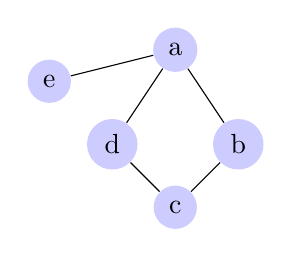
\begin{tikzpicture}
  [scale=.8,auto=left,every node/.style={circle,fill=blue!20}]
  \node (na) at (1,1.5) {a};
  \node (nb) at (2,0)  {b};
  \node (nc) at (1,-1)  {c};
  \node (nd) at (0,0) {d};
  \node (ne) at (-1,1)  {e};

  \foreach \from/\to in {na/nb,nb/nc,nc/nd,na/nd,na/ne}
    \draw (\from) -- (\to);

\end{tikzpicture}
\end{center}
\begin{defn}[planar graph]\label{planar graph}
A planar graph is a \nameref{graph} that can be drawn with no edges crossing.
\end{defn}
\end{exmp}
\begin{defn}[terminology]\label{terminology}
If $e = \{u,v\} \in E(G)$, we say
\begin{itemize}
  \item $u$ and $v$ are \textbf{adjacent}
  \item $e$ is \textbf{incident} with $u$
  \item $e$ is \textbf{incident} with $v$
  \item $e$ \textbf{joins} $u$ and $v$
  \item $v$ is a \textbf{neighbour} of $u$
\end{itemize}
\end{defn}

Some notes about the definition of a \nameref{graph}.
\begin{itemize}
  \item $V(G)$ is finite, we have no infinite \nameref{graph}s
  \item $E(G)$ is a set, we have no notion of multiple edges, e.g., we'll never have this
    \begin{center}
  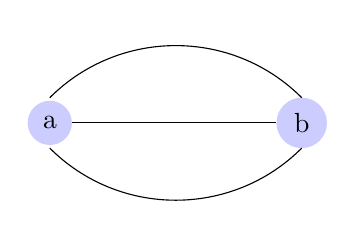
\begin{tikzpicture}
  [scale=.8,auto=left,every node/.style={circle,fill=blue!20}]
  \node (na) at (-2,0) {a};
  \node (nb) at (2,0)  {b};;

      \draw  (-2,0.4) to [out=45,in=135] (2,0.4);
      \draw  (-2,-0.4) to [out=-45,in=-135] (2,-0.4);
  \foreach \from/\to in {na/nb}
    \draw (\from) -- (\to);
\end{tikzpicture}
\end{center}
\item Edges and unordered pairs of verticies - edges don't have a direction (we don't draw arrows or anything on graphs)
\item Edges join \textbf{distinct} vertices
  \item $E(G)$ is a set, we have no notion of multiple edges, e.g., we'll never have this
    \begin{center}
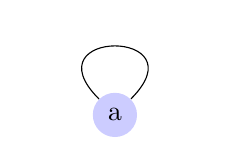
\begin{tikzpicture}[scale=.8,auto=left,every node/.style={circle,fill=blue!20}, every loop/.style={}]
    \node (3) {a};
    \path[every node/.style={font=\sffamily\small}]
        (3)   edge[loop] node  {} (3);
\end{tikzpicture}
\end{center}
\end{itemize}
People do study alternate / more general notions of \nameref{graph}s where these things are allowed, but not in this course.

\begin{exmp}
  Consider,
  \begin{center}
  $G_1, G_2, G_3, G_4$ \\
  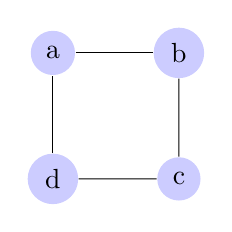
\begin{tikzpicture}
  [scale=.8,auto=left,every node/.style={circle,fill=blue!20}]
  \node (na) at (0,0) {a};
  \node (nb) at (2,0)  {b};
  \node (nc) at (2,-2) {c};
  \node (nd) at (0,-2) {d};;
  \foreach \from/\to in {na/nb,nb/nc,nc/nd,nd/na}
    \draw (\from) -- (\to);
\end{tikzpicture}
  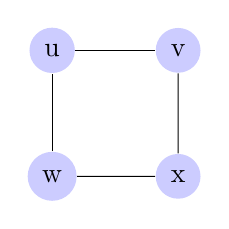
\begin{tikzpicture}
  [scale=.8,auto=left,every node/.style={circle,fill=blue!20}]
  \node (na) at (0,0) {u};
  \node (nb) at (2,0)  {v};
  \node (nc) at (2,-2) {x};
  \node (nd) at (0,-2) {w};;
  \foreach \from/\to in {na/nb,nb/nc,nc/nd,nd/na}
    \draw (\from) -- (\to);
\end{tikzpicture}
  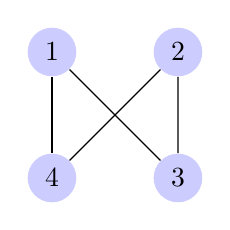
\begin{tikzpicture}
  [scale=.8,auto=left,every node/.style={circle,fill=blue!20}]
  \node (na) at (0,0) {1};
  \node (nb) at (2,0)  {2};
  \node (nc) at (2,-2) {3};
  \node (nd) at (0,-2) {4};;
  \foreach \from/\to in {na/nc,na/nd,nb/nd,nb/nc}
    \draw (\from) -- (\to);
\end{tikzpicture}
  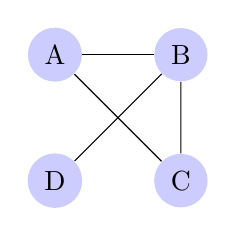
\begin{tikzpicture}
  [scale=.8,auto=left,every node/.style={circle,fill=blue!20}]
  \node (na) at (0,0) {A};
  \node (nb) at (2,0)  {B};
  \node (nc) at (2,-2) {C};
  \node (nd) at (0,-2) {D};;
  \foreach \from/\to in {na/nb,nb/nc,nc/na,nd/nb}
    \draw (\from) -- (\to);
\end{tikzpicture}
\end{center}
Note that $G_1, G_2$ and $G_3$ are essentially the same, but not equal, and $G_4$ is fundamentally different.
\begin{defn}[isomorphic]\label{isomorphic}
Two graphs $G_1$ and $G_2$ are \textbf{isomorphic} if there exists a bijection $f : V(G_1) \lar V(G_2)$ that preserved adjacencies, that is \[\{u,v\} \in E(G_1) \iff \{f(u), f(v) \} \in E(G_2)\]
THe bijection $f$ is called an \textbf{isomorphism}.
\end{defn}
\end{exmp}
\begin{exmp}
  From the above example, $f : V(G_1) \lar V(G_3)$ where $f(a) = 1$, $f(b) = 3$, $f(c) = 2$, $f(d) = 4$ is an isomorphism, it is \nameref{isomorphic}. Can you find a different isomorphism?
\end{exmp}
If $G_1$ and $G_2$ are isomorphic, they have all the same \textbf{features}. (anything you can define that doesn't involve specific vertex names)

\begin{defn}[degree]\label{degree}
If $G$ is a \nameref{graph} $u \in V(G)$, then the set of all \hyperref[terminology]{neighbours} of $u$ is denoted $N(u)$. The \textbf{degree} of $u$ is
\[ \deg(u) = |N(u)| \]
\end{defn}
\begin{defn}[degree sequence]\label{degree sequence}
The degree sequence of $G$ is the list of the degrees of the verticies of $G$ in decreasing order.
\end{defn}
\begin{exmp}
  The \nameref{degree sequence} of $G_1 : 2,2,2,2$, the \nameref{degree sequence} of $G_4 : 3,2,2,1$. This shows that $G_1$ and $G_4$ are \textbf{not} \nameref{isomorphic}.
\end{exmp}
To prove that two graphs are \nameref{isomorphic}, first state the isomorphism, then to find it line up the features. To prove that two \nameref{graph}s are not \nameref{isomorphic}, find some features that distinguish them. Another possibility is to use proof by contradiction; try to line up features and find none of the options work.

\subsection{Special Families of Graphs}

\begin{defn}[complete graph]\label{complete graph}
A complete \nameref{graph} $K_p$ for $p \in \N$ is a \nameref{graph} with $p$ vertices, and every pair of verticies is an adjacency. For example,
  \begin{center}
  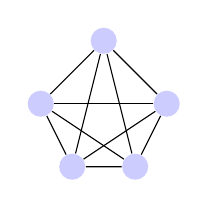
\begin{tikzpicture}
  [scale=.8,auto=left,every node/.style={circle,fill=blue!20}]
  \node (na) at (0,1) {};
  \node (nb) at (1,0)  {};
  \node (nc) at (-1,0)  {};
  \node (nd) at (-0.5,-1) {};
  \node (ne) at (0.5,-1)  {};

  \foreach \from/\to in {na/nb,na/ne,na/nd,na/nc,nb/nc,nb/nd,nb/nc,ne/nc,nd/ne,nd/nc, nb/ne}
    \draw (\from) -- (\to);

\end{tikzpicture}
\end{center}
so $|V(K_p)| = p$ and $|E(K_p)| = \comb{p}{2} = \f{p(p-1)}{2}$.
\end{defn}
There's also a graph at the other extreme with $p$ vertices and no edges.
  \begin{center}
  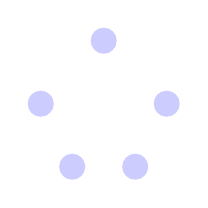
\begin{tikzpicture}
  [scale=.8,auto=left,every node/.style={circle,fill=blue!20}]
  \node (na) at (0,1) {};
  \node (nb) at (1,0)  {};
  \node (nc) at (-1,0)  {};
  \node (nd) at (-0.5,-1) {};
  \node (ne) at (0.5,-1)  {};
\end{tikzpicture}
\end{center}

\begin{defn}[$k$-regular]\label{k-regular}
A $k$-regular graph is a \nameref{graph} where every vertex has \nameref{degree} $k$. For example, $K_p$ is a $(p-1)$-regular \nameref{graph}. A $2$-regular graph example,
  \begin{center}
  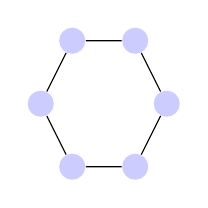
\begin{tikzpicture}
  [scale=.8,auto=left,every node/.style={circle,fill=blue!20}]
  \node (na) at (0.5,1) {};
  \node (nb) at (-0.5,1) {};
  \node (nc) at (1,0)  {};
  \node (nd) at (-1,0)  {};
  \node (ne) at (-0.5,-1) {};
  \node (nf) at (0.5,-1)  {};
    \foreach \from/\to in {na/nc,nc/nf,nf/ne,ne/nd,nd/nb, nb/na}
    \draw (\from) -- (\to);
\end{tikzpicture}
\end{center}
Also, the \textbf{Petersen} \nameref{graph} ($3$ regular)
  \begin{center}
  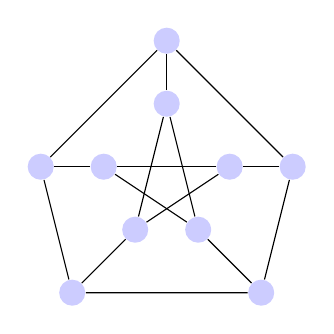
\begin{tikzpicture}
  [scale=.8,auto=left,every node/.style={circle,fill=blue!20}]
  \node (na) at (0,1) {};
  \node (nb) at (1,0)  {};
  \node (ne) at (-1,0)  {};
  \node (nd) at (-0.5,-1) {};
  \node (nc) at (0.5,-1)  {};
  \node (nA) at (0,2) {};
  \node (nB) at (2,0)  {};
  \node (nE) at (-2,0)  {};
  \node (nD) at (-1.5,-2) {};
  \node (nC) at (1.5,-2)  {};
    \foreach \from/\to in {nA/nB,nB/nC,nC/nD,nD/nE,nA/na,nB/nb,nC/nc,nD/nd,nE/ne,na/nc,nb/ne,nc/ne,nd/na,nE/nA, nd/nb}
    \draw (\from) -- (\to);
  \end{tikzpicture}
  \end{center}
  This can be drawn in another way, check the course notes.
\end{defn}

\begin{defn}[bipartite]\label{bipartite}
A bipartite \nameref{graph} is a \nameref{graph} where the vertices can be partitioned into two sets $A$ and $B$ where each edge is \hyperref[terminology]{incident} to one vertex in $A$ and one vertex in $B$. That is, each edge is of the form $\{a,b\}$ for $a \in A, b \in B$. For example,
  \begin{center}
  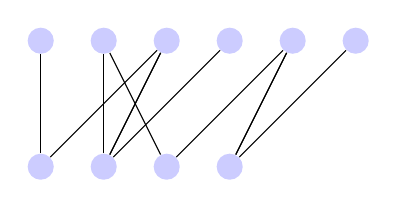
\begin{tikzpicture}
  [scale=.8,auto=left,every node/.style={circle,fill=blue!20}]
  \node (na) at (-2,1) {};
  \node (nb) at (-1,1) {};
  \node (nc) at (0,1)  {};
  \node (nd) at (1,1)  {};
  \node (ne) at (2,1) {};
  \node (nf) at (3,1) {};
  \node (nA) at (-2,-1) {};
  \node (nB) at (-1,-1) {};
  \node (nC) at (0,-1)  {};
  \node (nD) at (1,-1)  {};
    \foreach \from/\to in {na/nA,nA/nc,nc/nB,nB/nb,nb/nC,nC/ne,nD/ne,nB/nc,nB/nd,ne/nD,nD/nf}
    \draw (\from) -- (\to);
  \end{tikzpicture}
  \end{center}
  where the top row is $A$ and bottom row $B$. The pair $(A,B)$ is called a \textbf{bipartition}.
\end{defn}

\begin{defn}[complete bipartite]\label{complete bipartite}
A complete bipartite graph $K_{m,n}$ has a vertex set partitioned into $(A,B)$ where $|A| = m$ and $|B| = n$ and every vertex in $A$ is \hyperref[terminology]{adjacent} to every vertex in $B$. For example, $K_{3,4}$
  \begin{center}
  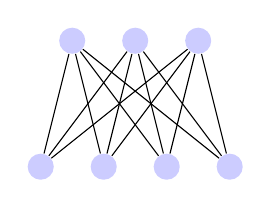
\begin{tikzpicture}
  [scale=.8,auto=left,every node/.style={circle,fill=blue!20}]
  \node (na) at (-1.5,1) {};
  \node (nb) at (-0.5,1) {};
  \node (nc) at (0.5,1)  {};
  \node (nA) at (-2,-1) {};
  \node (nB) at (-1,-1) {};
  \node (nC) at (0,-1)  {};
  \node (nD) at (1,-1)  {};
    \foreach \from/\to in {na/nA,na/nB,na/nC,na/nD, nb/nA,nb/nB,nb/nC,nb/nD,nc/nA,nc/nB,nc/nC,nc/nD}
    \draw (\from) -- (\to);
  \end{tikzpicture}
  \end{center}
  where $|V(K_{m,n})| = m + n$ and $|E(K_{m,n})| = mn$
\end{defn}

\begin{defn}[$n$-cube]\label{n-cube on}
A graph where vertices are $\{0,1\}$ strings of length $n$. Two strings are \hyperref[terminology]{adjacent} if they differ in exactly one position.
\begin{center}$O_2$
  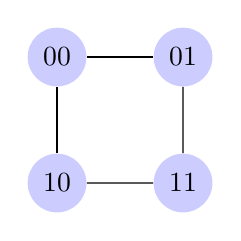
\begin{tikzpicture}
  [scale=.8,auto=left,every node/.style={circle,fill=blue!20}]
  \node (na) at (0,0) {00};
  \node (nb) at (2,0)  {01};
  \node (nc) at (2,-2) {11};
  \node (nd) at (0,-2) {10};;
  \foreach \from/\to in {na/nb,nb/nc,nc/nd,nd/na}
    \draw (\from) -- (\to);
\end{tikzpicture}
\end{center}
\begin{center}$O_3$
  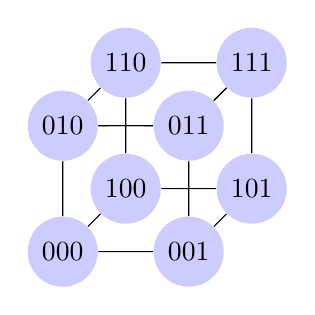
\begin{tikzpicture}
  [scale=.8,auto=left,every node/.style={circle,fill=blue!20}]
  \node (na) at (2,4) {110};
  \node (nb) at (4,4)  {111};
  \node (nc) at (1,3) {010};
  \node (nd) at (3,3) {011};
  \node (ne) at (1,1) {000};
  \node (nf) at (3,1)  {001};
  \node (ng) at (4,2) {101};
  \node (nh) at (2,2) {100};

  \foreach \from/\to in {nh/na,na/nb,na/nc,nc/nd,nb/nd,ne/nh,ne/nf,nf/ng,nd/nb,nd/nc,nd/nf,ne/nc,ng/nb,ng/nh}
    \draw (\from) -- (\to);
\end{tikzpicture}
\end{center}
$O_n$ is $n$-regular (each vertex has $n$ positions that could be changed to get an \hyperref[terminology]{incident} edge).
\end{defn}
\begin{thrm}
  $O_n$ is also \nameref{bipartite}.
\end{thrm}
\begin{proof}
  Let $A = $ strings with an even number of 1s, and $B$ the same with odd number of 1s. THen every edge connects two strings, one of which has $k$ 1s andthe other has $k + 1$ 1s, so one is in $A$ and the other is in $B$.
\end{proof}
\begin{thrm}
  If a \nameref{graph} $G$ has $q$ edges, then
  \[ \sum_{v \in V(G)} \deg(v) = 2q \]
\end{thrm}
\begin{proof}
  Each edge is \hyperref[terminology]{incident} with verticies. So we sum the degrees of the verticies, we count each edge twice.
\end{proof}
\begin{cor}
  Every \nameref{graph} has an even number of \hyperref[terminology]{vertices} of odd \nameref{degree}.
\end{cor}
How many edges, verticies does $O_n$ have?
\[ |V(O_n)| = 2^n \]
\[ |E(O_n)| = q \]
We apply the theorem,
\[ \sum_{v \in V(G)} \deg(v) = 2q  \]
Since $\deg(v) = n$ for all $v \in V(O_n)$, $2^n \cdot n = 2q$ therefore $q = n2^{n-1}$.
\begin{exmp}
  The Petersen \nameref{graph} is a 3-regular graph with 10 verticiesl. Can you find a 3-regular graph with 11 verticies? \\

  The answer is that you can't becuase if $G$ were such a graph it would mean that
  \[ \sum_{v \in V(G)} \deg (v) = 3 \cdot 11 = 33 \not = 2q \]
\end{exmp}

\subsection{Paths and Walks}

\begin{defn}[walk]\label{walk}
Let $x$ and $y$ be  \hyperref[terminology]{vertices} in a graph $G$. A \textbf{walk} from $x$ to $y$ is  an alternating sequence of \hyperref[graph]{vertices} and \hyperref[graph]{edges}
\[ v_0e_1v_1e_2v_2e_3v_3\cdots v_{n-1}e_nv_n \]
where \begin{itemize}
  \item $v_0,\ldots,v_n \in V(G)$ and
  \item $e_1,\ldots,e_n \in E(G)$, and
  \item  $e_i = \{v_{i-1},v_i\}$ joins $v_{i-1}$ and $v_i$
  \item $x = v_0, y = v_n$
\end{itemize}
Sometimes this becomes cumbersome and a walk is described by listing vertices:
\[ v_0v_1v_2\cdots v_n \]
\end{defn}
\begin{defn}[length]\label{length}
In the above definition, $n$ is called the \textbf{length} of the \nameref{walk}. (It is the number of edges in the sequence). For example,
\begin{center}
  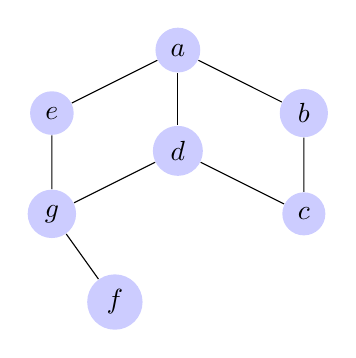
\begin{tikzpicture}
  [scale=.8,auto=left,every node/.style={circle,fill=blue!20}]
  \node (na) at (0,5) {$a$};
  \node (nb) at (2,4)  {$b$};
  \node (nc) at (-2,4) {$e$};
  \node (nd) at (0,3.4) {$d$};
  \node (ne) at (-2,2.4) {$g$};
  \node (nf) at (2,2.4)  {$c$};
  \node (ng) at (-1,1) {$f$};

  \foreach \from/\to in {na/nc,na/nb,na/nd,nd/ne,ng/ne,nb/nf,nd/nf,ne/nc}
    \draw (\from) -- (\to);
\end{tikzpicture}
\end{center}
where $abcbcdgfgdae$ is a \nameref{walk} from $a$ to $e$ of \nameref{length} 11.
\end{defn}

\begin{defn}[path]\label{path}
A \textbf{path} in $G$ from $x$ to $y$ is a \nameref{walk} in which no vertices are repeated.
\end{defn}

\begin{thrm}
  If there is a \nameref{walk} from $x$ to $y$ in $G$ then there is a path from $x$ to $y$ in $G$.
\end{thrm}

\begin{proof}
  Let $v_0v_1v_2\cdots v_n$ be a \nameref{walk} from $x$ to $y$. Perform the following algorithm on this \nameref{walk}: \\
  If this is a \nameref{path}, STOP. \\
  Otherwise, there must be a vertex repeated, say $v_i = v_j$ for $i \not = j$. This means $v_0v_1\cdots v_iv_{j+1}v_{j+2}\cdots v_n$ is a \nameref{walk} from $x$ to $y$. \\
  Repeat, with this \nameref{walk}. \\
  Since the \nameref{walk} gets shorter each time we run through the loop, the algorithm must stop. But, it stops when we have a \nameref{path} from $x$ to $y$. Therefore, there is a \nameref{path} from $x$ to $y$.
\end{proof}

Here is a question, what happens in this algorithm if the \nameref{walk} is something like this:
\[ v_0v_1v_2 \]
where $v_0 = a$, $v_1 = b$, $v_2 = a$ and we have a graph
\begin{center}
  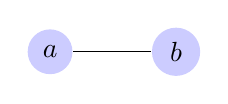
\begin{tikzpicture}
  [scale=.8,auto=left,every node/.style={circle,fill=blue!20}]
  \node (na) at (0,0) {$a$};
  \node (nb) at (2,0)  {$b$};

  \foreach \from/\to in {na/nb}
    \draw (\from) -- (\to);
\end{tikzpicture}
\end{center}
\begin{cor}
  If there is a \nameref{path} from $x$ to $y$, and a \nameref{path} from $y$ to $z$, there is a path from $x$ to $z$.
\end{cor}

\begin{proof}
  Let $u_0u_1\cdots u_m$ be a \nameref{path} from $x$ to $y$ and let $v_0 v_1 \cdots v_n$ be a \nameref{path} from $y$ to $z$. Then $u_0u_1\cdots u_m v_1 v_2 \cdots v_n$ is a \nameref{walk} from $x$ to $z$. Therefore since there is a \nameref{walk} from $x$ to $z$ there's a \nameref{path} from $x$ to $z$.
\end{proof}

\begin{thrm}
  The relation on $V(G)$ given by $x \sim y$ if there is a \nameref{walk} (or a \nameref{path}) from $x$ to $y$ iis an equivalence relation.
\end{thrm}
\begin{note}
  Think of an equivalence relation as putting the elements of a set into groups. (equivalence classes)
\end{note}

\begin{defn}[connected]\label{connected}
  We day that a \nameref{graph} is \textbf{connected} if this equivalence relation has one equivalence class. That is, for any two vertices $x,y \in V(G)$ there is a \nameref{walk}/\nameref{path} from $x$ to $y$.
\end{defn}
\begin{exmp}
  \begin{center}
  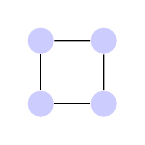
\begin{tikzpicture}
  [scale=.8,auto=left,every node/.style={circle,fill=blue!20}]
  \node (na) at (0,0) {};
  \node (nb) at (1,0) {};
  \node (nc) at (1,1) {};
  \node (nd) at (0,1) {};

  \foreach \from/\to in {na/nb,nb/nc,nc/nd,nd/na}
    \draw (\from) -- (\to);
\end{tikzpicture}
\end{center}
This is an example of a connected graph.
\end{exmp}
\begin{exmp}
    \begin{center}
  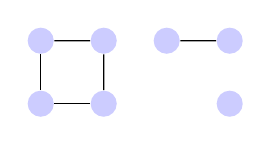
\begin{tikzpicture}
  [scale=.8,auto=left,every node/.style={circle,fill=blue!20}]
  \node (na) at (0,0) {};
  \node (nb) at (1,0) {};
  \node (nc) at (1,1) {};
  \node (nd) at (0,1) {};
  \node (ne) at (2,1) {};
  \node (nf) at (3,1) {};
  \node (ng) at (3,0) {};
  \foreach \from/\to in {na/nb,nb/nc,nc/nd,nd/na,ne/nf}
    \draw (\from) -- (\to);
\end{tikzpicture}
\end{center}
This graph is not connected.
\end{exmp}

\begin{thrm}\label{vertextopath}
  Suppose there is a vertex $v \in V(G)$ such that for every vertex $u \in V(G)$ there is a \nameref{path} from $u$ to $v$ in $G$. Then $G$ is \nameref{connected}. Kevin Purbhoo calls this the "Hub Model".
\end{thrm}

\begin{proof}
  Let $x$ and $y$ be any two vertices of $V(G)$, sicne there is a \nameref{walk} from $x$ to $y$, and a \nameref{walk} from $v$ to $y$, there is a \nameref{walk} from $x$ to $y$. This proves that $G$ is \nameref{connected}.
\end{proof}

\begin{note}
  If there is a \nameref{walk} from $x$ to $y$, then there is a \nameref{walk} from $y$ to $x$.
\end{note}

\begin{exmp}
  Prove that the \nameref{n-cube on} is \nameref{connected}.
  \begin{proof}
    Let $v = \ub{000\ldots0}_n \in V(O_n)$. Let $x$ be any vertex of $O_n$. Let $i_1,i_2,\ldots,i_k$ be the positions of the 1s in $x$. For $j = 0,\ldots,k$, let $v_j$ be the $\{0,1\}$-string that has 1s in positions $i_1,i_2,\ldots,i_j$ and 0s elsewhere. Then $v_0 = 00\ldots 0 = v$ and $v_k = x$. And so $v_0v_1v_2\cdots v_k$ is a \nameref{path} from $v$ to $x$. By \autoref{vertextopath}, this proves that the \nameref{n-cube on} is \nameref{connected}.
  \end{proof}
\end{exmp}

\subsection{Subgraphs}

\begin{defn}[subgraph]\label{subgraph}
Let $G$ be a \nameref{graph}. A \textbf{subgraph} of $G$ is a \nameref{graph} $H$ such that $V(H) \subseteq V(G)$ and $E(H) \subseteq E(G)$.
\end{defn}

\begin{exmp}
  A \nameref{graph}.
    \begin{center}
  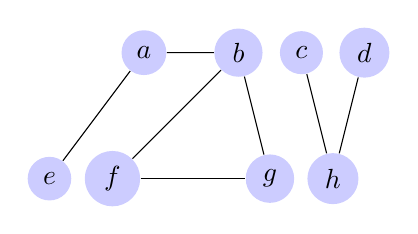
\begin{tikzpicture}
  [scale=.8,auto=left,every node/.style={circle,fill=blue!20}]
  \node (ne) at (-1,0) {$e$};
  \node (na) at (0.5,2) {$a$};
  \node (nb) at (2,2) {$b$};
  \node (ng) at (2.5,0) {$g$};
  \node (nf) at (0,0) {$f$};
  \node (nc) at (3,2) {$c$};
  \node (nd) at (4,2) {$d$};
  \node (nh) at (3.5,0) {$h$};
  \foreach \from/\to in {na/ne,na/nb,nb/ng,nb/nf,nf/ng,nc/nh,nh/nd}
    \draw (\from) -- (\to);
\end{tikzpicture}
\end{center}
A \nameref{subgraph} example could be
  A \nameref{graph}.
    \begin{center}
  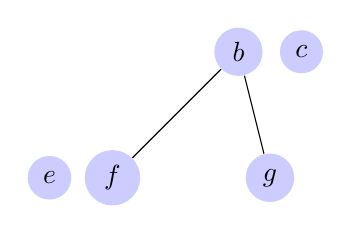
\begin{tikzpicture}
  [scale=.8,auto=left,every node/.style={circle,fill=blue!20}]
  \node (ne) at (-1,0) {$e$};
  \node (nb) at (2,2) {$b$};
  \node (ng) at (2.5,0) {$g$};
  \node (nf) at (0,0) {$f$};
  \node (nc) at (3,2) {$c$};
  \foreach \from/\to in {nb/ng,nb/nf}
    \draw (\from) -- (\to);
\end{tikzpicture}
\end{center}
Note that every edge in $E(H)$ must have both ends in $V(H)$.
\end{exmp}

\begin{defn}[spanning]\label{spanning}
A \nameref{subgraph} $H$ of $G$ is \textbf{spanning} if $V(H) = V(G)$
\end{defn}

For example,
    \begin{center}
  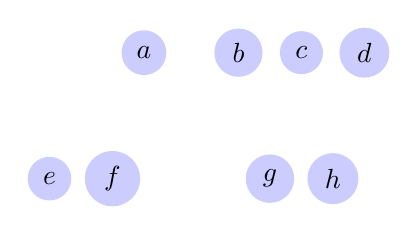
\begin{tikzpicture}
  [scale=.8,auto=left,every node/.style={circle,fill=blue!20}]
  \node (ne) at (-1,0) {$e$};
  \node (na) at (0.5,2) {$a$};
  \node (nb) at (2,2) {$b$};
  \node (ng) at (2.5,0) {$g$};
  \node (nf) at (0,0) {$f$};
  \node (nc) at (3,2) {$c$};
  \node (nd) at (4,2) {$d$};
  \node (nh) at (3.5,0) {$h$};
\end{tikzpicture}
\end{center}
is a spanning subgraph of the graph above. \\

Also, not relevant to this course, but a \nameref{subgraph} where $E(H)$ uses all edges that make sense is called \textbf{induced.}

\begin{defn}[component]\label{component}
A \textbf{component} of a \nameref{graph} $G$ is a \nameref{subgraph} $H$ such that $H$ is \nameref{connected}. Any \nameref{subgraph} of $G$ that properly contains $H$ is not \nameref{connected}.
\end{defn}
\begin{exmp}
A graph with four components,
  \begin{center}
  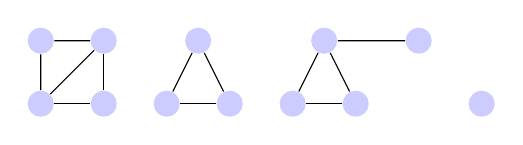
\begin{tikzpicture}
  [scale=.8,auto=left,every node/.style={circle,fill=blue!20}]
  \node (a) at (-1,1) {};
  \node (b) at (-1,0) {};
  \node (c) at (0,1) {};
  \node (d) at (0,0) {};
  \node (e) at (1,0) {};
  \node (f) at (1.5,1) {};
  \node (g) at (2,0) {};
  \node (h) at (3,0) {};
  \node (i) at (3.5,1) {};
  \node (j) at (4,0) {};
  \node (k) at (5,1) {};
   \node (l) at (6,0) {};
  \foreach \from/\to in {a/b,b/c,b/d,a/c,c/d,e/f,e/g,f/g,h/i,h/j,i/j,i/k}
    \draw (\from) -- (\to);
\end{tikzpicture}
\end{center}
\end{exmp}

\textbf{Fact.} A \nameref{graph} is \nameref{connected} if it has exactly one \nameref{component}. This follows from definitions.

\begin{defn}[cut]\label{cut}
Let $G$ be a \nameref{graph} and let $X \subseteq V(G)$. The \textbf{cut} on $X$ is the set of all edges $e \in E(G)$ that have exactly one vertex in $X$.
\end{defn}

\begin{note}
  Drawing these graphs is a little tedious for me, I'll add them later, check the course notes for now.
\end{note}
% \begin{exmp}
%     \begin{center}
%   \begin{tikzpicture}
%   [scale=.8,auto=left,every node/.style={circle,fill=blue!20}]
%   \node (a) at (-1,1) {};
%   \node (b) at (-1,0) {};
%   \node (c) at (0,1) {};
%   \node (d) at (0,0) {};
%   \node (e) at (1,0) {};
%   \node (f) at (1.5,1) {};
%   \node (g) at (2,0) {};
%   \node (h) at (3,0) {};
%   \node (i) at (3.5,1) {};
%   \node [minimum size=2cm] (j) at (4,0) {};
%   \node (k) at (5,1) {};
%    \node (l) at (6,0) {};
%   \foreach \from/\to in {a/b,b/c,b/d,a/c,c/d,e/f,e/g,f/g,h/i,h/j,i/j,i/k}
%     \draw [decorate,decoration=zigzag] (\from) -- (\to);
% \end{tikzpicture}
% \end{center}
% \end{exmp}

\begin{thrm}
 Let $G$ be a \nameref{graph}. If there is a proper, non-empty subset $X \subset V(G)$, such that the \nameref{cut} on $X$ is empty, then $G$ is not \nameref{connected}.
\end{thrm}

That is, how to prove a \nameref{graph} is not \nameref{connected}.
\begin{itemize}
  \item Find a proper, non-empty subset $X \subset V(G)$
  \item Check that for every edge $e \in E(G)$, either $e$ joins two vertices in $X$, or $e$ joins two vertices in $V(G) \setminus X$.
  \item How to get $X$? Take $X$ to be all vertices in one \nameref{component}. If $X$ has more than one \nameref{component} this works, because $X$ is proper $(X \not = V(G))$ and $X = \emptyset$.
\end{itemize}

\begin{proof}(of Theorem 4.6)
  Let $x \in X$, $y \in V(G) \setminus X$. We show that if the \nameref{cut} on $X$ is empty, there is no \nameref{path} from $x$ to $y$. Suppose to the contrary that we had such a \nameref{path} $v_0v_1v_2\cdots v_n$, where $v_0 = x$, $v_n = y$. \\
  Let $i$ be the the largest index such that $v_i \in X$. Note that $i < n$ because $v_n \not \in X$ so $v_{i+1} \in V(G) \setminus X$, and $\{v_i, v_{i+1}\} \in E(G)$. So, $\{v_i, v_{i+1} \}$ belongs to the \nameref{cut} on $X$. This contradicts our assumption that \nameref{cut} on $X$ is empty.
\end{proof}

The converse is also true: If $G$ is not \nameref{connected}, then we can find a proper non-empty subset $X \subset V(G)$, such that the \nameref{cut} on $X$ is empty. \\

\textbf{Idea:} Take $X = V(H)$, where $H$ is a \nameref{component}, argue that this works.

\subsection{Cycles and Bridges}

\begin{defn}[cycle]\label{cycle}
A \textbf{cycle} is a \nameref{graph} $C$ with $n$ vertices $V(C) = \{v_0, v_1, \ldots, v_{n-1}\}$ and $m$ edges $E(C) = \{ \{v_0, v_1\}, \{v_1, v_2\}, \{v_2,v_3\}, \ldots, \{v_{n-2}, v-{n-1}\}, \{v_{n-1}, v_0\}\}$. For example, a cycle with 7 vertices and edges - also called a 7-cycle.
  \begin{center}
  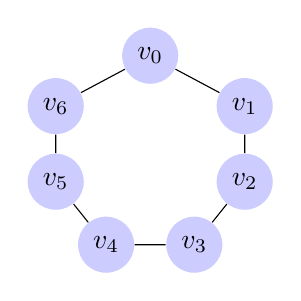
\begin{tikzpicture}
  [scale=.8,auto=left,every node/.style={circle,fill=blue!20}]
  \node (a) at (0.5,4) {$v_0$};
  \node (b) at (2,3.2) {$v_1$};
  \node (c) at (2,2) {$v_2$};
  \node (d) at (1.2,1) {$v_3$};
  \node (e) at (-0.2,1) {$v_4$};
  \node (f) at (-1,2) {$v_5$};
  \node (g) at (-1,3.2) {$v_6$};
  \foreach \from/\to in {a/b,b/c,c/d,d/e,e/f,f/g,g/a}
    \draw (\from) -- (\to);
\end{tikzpicture}
\end{center}
Note that a \nameref{cycle} can't have \nameref{length} 1 or 2.
\begin{itemize}
  \item Length 1 : requires edge $\{v_0, v_0\}$ (not allowed)
  \item Length 2 : requires 2 edges $\{\{v_0,v_1\},\{v_1,v_0\}\}$ (just one edge)
\end{itemize}
\end{defn}
\begin{defn}[subcycle]\label{subcycle}
If $G$ is a \nameref{graph}, a \nameref{cycle} in $G$ is a \nameref{subgraph} of $G$ that is a \nameref{cycle}. For example,
 \begin{center}
  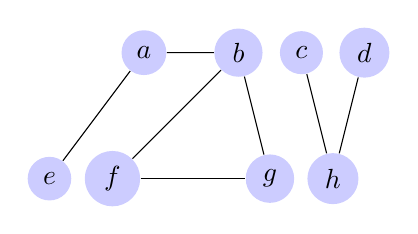
\begin{tikzpicture}
  [scale=.8,auto=left,every node/.style={circle,fill=blue!20}]
  \node (ne) at (-1,0) {$e$};
  \node (na) at (0.5,2) {$a$};
  \node (nb) at (2,2) {$b$};
  \node (ng) at (2.5,0) {$g$};
  \node (nf) at (0,0) {$f$};
  \node (nc) at (3,2) {$c$};
  \node (nd) at (4,2) {$d$};
  \node (nh) at (3.5,0) {$h$};
  \foreach \from/\to in {na/ne,na/nb,nb/ng,nb/nf,nf/ng,nc/nh,nh/nd}
    \draw (\from) -- (\to);
\end{tikzpicture}
\end{center}
There is a subcycle between vertices $b, f$, and $g$.
\end{defn}
An easier way to specify a \nameref{cycle} is to write down a \nameref{walk} around the \nameref{cycle}. For example, $v_0v_1v_2\cdots v_{n-1}v_0$. This is a \textbf{closed walk}, meaning that it starts and ends at the same vertex. \\

Cycles are "more than connected". Consider
  \begin{center}
  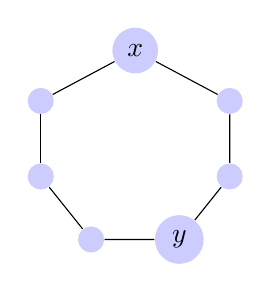
\begin{tikzpicture}
  [scale=.8,auto=left,every node/.style={circle,fill=blue!20}]
  \node (a) at (0.5,4) {$x$};
  \node (b) at (2,3.2) {};
  \node (c) at (2,2) {};
  \node (d) at (1.2,1) {$y$};
  \node (e) at (-0.2,1) {};
  \node (f) at (-1,2) {};
  \node (g) at (-1,3.2) {};
  \foreach \from/\to in {a/b,b/c,c/d,d/e,e/f,f/g,g/a}
    \draw (\from) -- (\to);
\end{tikzpicture}
\end{center}
There are almost completely disjoint \nameref{path}s from $x$ to $y$. \\

\textbf{Cycles and Bipartite Graphs} \\

If $G$ is a \nameref{bipartite} \nameref{graph}, then any \nameref{subgraph} of $G$ is a \nameref{bipartite} \nameref{graph}. Every \nameref{cycle} in $G$ is a \nameref{bipartite} \nameref{graph}. When is a \nameref{cycle} \nameref{bipartite}? Consider this graph,
  \begin{center}
  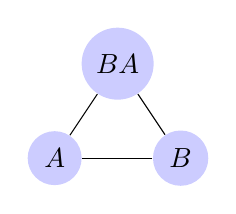
\begin{tikzpicture}
  [scale=.8,auto=left,every node/.style={circle,fill=blue!20}]
  \node (a) at (0,1.5) {$BA$};
  \node (b) at (1,0) {$B$};
  \node (c) at (-1,0) {$A$};
  \foreach \from/\to in {a/b,b/c,c/a}
    \draw (\from) -- (\to);
\end{tikzpicture}
\end{center}
This is not \nameref{bipartite} (like we have shown by labelling $BA$ on the top node). Additionally, a graph with 5 vertices is not \nameref{bipartite}. Consider,
\begin{center}
  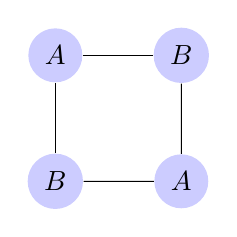
\begin{tikzpicture}
  [scale=.8,auto=left,every node/.style={circle,fill=blue!20}]
  \node (na) at (0,0) {$A$};
  \node (nb) at (2,0)  {$B$};
  \node (nc) at (2,-2) {$A$};
  \node (nd) at (0,-2) {$B$};;
  \foreach \from/\to in {na/nb,nb/nc,nc/nd,nd/na}
    \draw (\from) -- (\to);
\end{tikzpicture}
\end{center}
This \nameref{graph} is \nameref{bipartite}, so we conclude that for a \nameref{cycle} to be \nameref{bipartite}, it must have an even number of vertices.

\begin{thrm}
  Even \nameref{cycle}s are \nameref{bipartite}. Odd \nameref{cycle}s are not \nameref{bipartite}.
\end{thrm}
\begin{proof}
  Let $C$ be an $n$-\nameref{cycle} and let $v_0v_1\cdots v_{n-1}v_0$ be a \nameref{walk} around $C_1$. If $n$ is even, let $A = \{v_0,v_2,\ldots,v_{n-2}\}$ and $B = \{v_1,v_3,\ldots,v_{n-1}\}$ then $(A,B)$ is a bipartition. If $n$ is odd, we can try to cosntruct a bipartition. Without loss of generality, let $v_0 \in A$. Then $v_1 \in B$, $v_2 \in A, v_3 \in B$, and in general we can easily show that $v_1 \in A$ if $i$ is even and $v_i \in B$ if $i$ is odd. But since $n$ is odd, $v_0, v_{n-1} \in A$ and $\{v_0, v_{n-1} \} \in E(C)$. So this is not a bipartition. Therefore, there is no bipartition.
\end{proof}

\begin{cor}
  If $G$ has an odd \nameref{cycle}, then $G$ is not bipartite.
\end{cor}

 \begin{proof}
   We just discuss how we can't have a non-\nameref{bipartite} \nameref{subgraph} of a \nameref{bipartite} \nameref{graph}. If we had an odd \nameref{cycle} in a \nameref{bipartite} \nameref{graph}, we'd have a massive contradiction.
 \end{proof}

 \begin{defn}[edge deletion]\label{edge deletion}
 Let $G$ be a \nameref{graph} and $e \in E(G)$. Then $G - e$ is the \nameref{subgraph} $G$ with $V(G - e) = V(G)$ and $E(G-e) = E(G) \setminus \{e\}$.
 \end{defn}

 \begin{exmp} Consider $G$,
     \begin{center}
  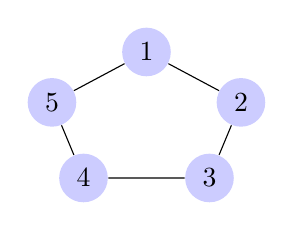
\begin{tikzpicture}
  [scale=.8,auto=left,every node/.style={circle,fill=blue!20}]
  \node (a) at (0.5,4) {$1$};
  \node (b) at (2,3.2) {$2$};
  \node (c) at (1.5,2) {$3$};
  \node (d) at (-0.5,2) {$4$};
  \node (e) at (-1,3.2) {$5$};
  \foreach \from/\to in {a/b,b/c,c/d,d/e,e/a}
    \draw (\from) -- (\to);
\end{tikzpicture}
\end{center}
where $e = \{2,3\}$. Then $G - e$ looks like
     \begin{center}
  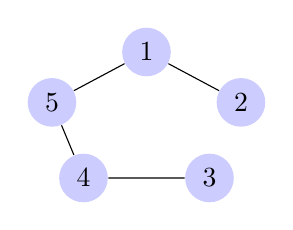
\begin{tikzpicture}
  [scale=.8,auto=left,every node/.style={circle,fill=blue!20}]
  \node (a) at (0.5,4) {$1$};
  \node (b) at (2,3.2) {$2$};
  \node (c) at (1.5,2) {$3$};
  \node (d) at (-0.5,2) {$4$};
  \node (e) at (-1,3.2) {$5$};
  \foreach \from/\to in {a/b,c/d,d/e,e/a}
    \draw (\from) -- (\to);
\end{tikzpicture}
\end{center}
 \end{exmp}

 \begin{defn}[bridge]\label{bridge}
 Let $e \in E(G)$. We say that $e$ is a \textbf{bridge} if $G - e$ has more \nameref{component}s than $G$.
 \end{defn}

 \begin{exmp}
   Consider $G$ with $e = \{3,4\}$.
    \begin{center}
  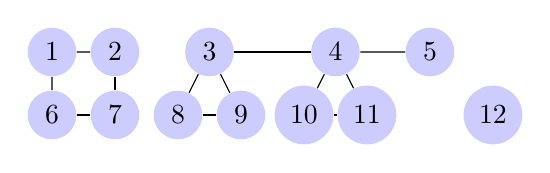
\begin{tikzpicture}
  [scale=.8,auto=left,every node/.style={circle,fill=blue!20}]
  \node (a) at (-1,1) {1};
  \node (b) at (-1,0) {6};
  \node (c) at (0,1) {2};
  \node (d) at (0,0) {7};
  \node (e) at (1,0) {8};
  \node (f) at (1.5,1) {3};
  \node (g) at (2,0) {9};
  \node (h) at (3,0) {10};
  \node (i) at (3.5,1) {4};
  \node (j) at (4,0) {11};
  \node (k) at (5,1) {5};
   \node (l) at (6,0) {12};
  \foreach \from/\to in {a/b,b/d,a/c,c/d,e/f,e/g,f/g,h/i,h/j,i/j,i/k,f/i}
    \draw (\from) -- (\to);
\end{tikzpicture}
\end{center}
Which has 3 \nameref{component}s. Then $G - e$,
    \begin{center}
  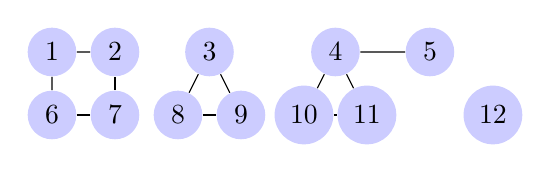
\begin{tikzpicture}
  [scale=.8,auto=left,every node/.style={circle,fill=blue!20}]
  \node (a) at (-1,1) {1};
  \node (b) at (-1,0) {6};
  \node (c) at (0,1) {2};
  \node (d) at (0,0) {7};
  \node (e) at (1,0) {8};
  \node (f) at (1.5,1) {3};
  \node (g) at (2,0) {9};
  \node (h) at (3,0) {10};
  \node (i) at (3.5,1) {4};
  \node (j) at (4,0) {11};
  \node (k) at (5,1) {5};
   \node (l) at (6,0) {12};
  \foreach \from/\to in {a/b,b/d,a/c,c/d,e/f,e/g,f/g,h/i,h/j,i/j,i/k}
    \draw (\from) -- (\to);
\end{tikzpicture}
\end{center}
has 4-\nameref{component}s.
 \end{exmp}

 \begin{lem}
   Let $G$ be a \nameref{connected} \nameref{graph} and let $e = \{x,y\}$ be an edge. If $e$ is a \nameref{bridge}, then $G - e$ has \textbf{exactly} 2 \nameref{component}s and $x$ and $y$ are in different \nameref{component}s.
 \end{lem}

\begin{proof}
  Let $z \in V(G) = V(G - e)$. We will show that there is either a \nameref{path} from $x$ to $z$ in $G - e$ or a \nameref{path} from $y$ to $z$ in $G - e$. Since $G$ is \nameref{connected}, there is a \nameref{path} from $x$ to $z$ in $G$. If $e$ is not in this \nameref{path}, then this is a \nameref{path} in $G - e$ from $x$ to $z$. Otherwise, the \nameref{path} is of the form
  \[ x\cdots ev_k \cdots z \]
  Since $e$ can't appear twice, $v_k\cdots z$ is a \nameref{path} in $G-e$ and $v_k \in \{x, y\} = e$. \\
  So in either case, we have either a \nameref{path} from $x$ to $z$ or from $y$ to $z$ in $G - e$. This shows that every vertex of $G - e$ is either in the \nameref{component} of $x$ or the \nameref{component} of $y$. Therefore $G - e$ has at most 2 \nameref{component}s. \\
  Since $e$ is a bridge, $G - e$ has at least two \nameref{component}s. The result follows.
\end{proof}

\textbf{Generalization.} Let $G$ be any \nameref{graph}. If $e = \{x,y\} \in E(G)$ is a \nameref{bridge}, then $G - e$ has exactly one more \nameref{component} than $G$, and $x$ and $y$ are in different \nameref{component}s of $G - e$.

\begin{proof}
  Component of $e$ splits in two other componenets unchanged in $G -e$.
\end{proof}

\begin{thrm}
  Let $e \in E(G)$ be an edge of a \nameref{graph} $G$. Then $e$ is a \nameref{bridge} if and only if $e$ is not contained in any \nameref{cycle}.
\end{thrm}

\begin{proof}
  Suppose to the contrary, that $e$ is contained in a \nameref{cycle}, say the \nameref{cycle} is given by the \nameref{walk}:
  \[ xeye_1 v_1e_2v_2\cdots x \]
  Then $ye_1v_1e_2v_2 \cdots x$ is a \nameref{path} in $G - e$ from $y$ to $x$. So $y$ and $x$ are in the same \nameref{component} of $G -e$. By the lemma, $e$ cannot be a \nameref{bridge}. \\

  In the other direction, suppose $e$ is not a \nameref{bridge}, then $x$ and $y$ are in the same \nameref{component} of $G - e$, therefore there is a \nameref{path} $ye_1v_1e_2v_2 \cdots x$ in $G - e$. Then, $xeye_1v_1e_2v_2 \cdots x$ is a \nameref{walk} around a \nameref{cycle}. Therefore $e$ is contained in a \nameref{cycle}.
\end{proof}

  \begin{center}
  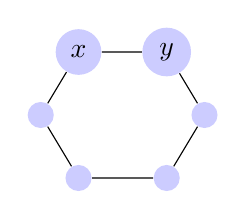
\begin{tikzpicture}
  [scale=.8,auto=left,every node/.style={circle,fill=blue!20}]
  \node (a) at (0.8,4) {$x$};
  \node (b) at (2.2,4) {$y$};
  \node (c) at (2.8,3) {};
  \node (d) at (2.2,2) {};
  \node (e) at (0.8,2) {};
  \node (f) at (0.2,3) {};
  \foreach \from/\to in {a/b,b/c,c/d,d/e,e/f,f/a}
    \draw (\from) -- (\to);
\end{tikzpicture}
\end{center}

where the edge between $x$ and $y$ is $e$.

\begin{thrm}
  Let $G$ be a \nameref{graph}. If there are two vertices $u$ and $v$ of $G$ such that there are two different paths from $u$ to $v$, then $G$ contains a \nameref{cycle}.
\end{thrm}
\begin{proof}
  Let $P_1 = ux_1x_2x_3\cdots x_{k-1}v$ and $P_2 = uy_1y_2y_3\cdots y_{l-1} v$. Since a path from $u$ to $v$ is determined by the set of edges it uses, $P_1$ and $P_2$ can't use the same set of edges. These must be an edge $e$ that appears in one but not the other. Without loss of generality, say $P_1 = u \cdots x_i e x_{i+1}\cdots v$ and $e$ not in $P_2$. Then $x_ix_{i-1}\cdots u y_1 y_2 \cdots v y_{k-1} \cdots x_{i+1}$ is a \nameref{walk} from $x_i$ to $x_{i+1}$ that does not use $e$. Therefore $x_i$ and $x_{i+1}$ are in the same \nameref{component} of $G - e$. Therefore $e$ is not a \nameref{bridge}, $e$ is in a \nameref{cycle}, and so $G$ has a \nameref{cycle}.
\end{proof}
Essentially we have shown, to summarize,
\[ \mbox{$e$ is a \nameref{bridge}} \iff \mbox{$e$ is not a \nameref{cycle}} \]
\[ \mbox{\nameref{cycle}} \iff \mbox{two \nameref{path}s between $u$ and $v$} \]
\subsection{Trees}

\begin{defn}[tree]\label{tree}
A \textbf{tree} is a \nameref{connected} \nameref{graph} with no \nameref{cycle}s. For example,
  \begin{center}
  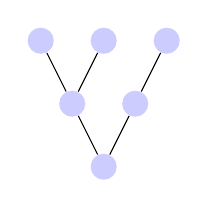
\begin{tikzpicture}
  [scale=.8,auto=left,every node/.style={circle,fill=blue!20}]
  \node (a) at (0,4) {};
  \node (b) at (1,4) {};
  \node (c) at (2,4) {};
  \node (e) at (0.5,3) {};
  \node (d) at (1.5,3) {};
  \node (f) at (1,2) {};
  \foreach \from/\to in {f/e,f/d,e/a,e/b,d/c}
    \draw (\from) -- (\to);
\end{tikzpicture}
\end{center}
\end{defn}

Some properties of \nameref{tree}s,
\begin{itemize}
  \item[1.] There is a unique \nameref{path} between any two vertices.
  \begin{proof}
    Let $T$ be a \nameref{tree}. Since $T$ is \nameref{connected} there is at least one \nameref{path} between any two vertices. If there were two, one would have a \nameref{cycle}.
  \end{proof}
  \item[2.] Every edge of $T$ is a \nameref{bridge}.
  \begin{proof}
    If $T$ had an edge that was not a \nameref{bridge}, that edge would be in a \nameref{cycle}.
  \end{proof}
  \item[3.] If a \nameref{tree} has $p$ vertices, then it has $q = p - 1$ edges.
  \begin{proof}
    By strong induction on $p$, the number of vertices. If $p = 1$ then any \nameref{graph} with one vertex has 0 edges, so the result is true. Fix $p > 1$, assume the result is true for all \nameref{tree}s with fewer than $p$ vertices. Let $T$ be a \nameref{tree} with $p$ vertices, we want to prove that $T$ has $p - 1$ edges. Let $e \in E(T)$. Then $e$ is a \nameref{bridge}. So, $T - e$ has two \nameref{component}s, call them $T_1$ and $T_2$. $T_1$ and $T_2$ are \nameref{connected} (because they're \nameref{component}s) and have no \nameref{cycle}s, because they are \nameref{subgraph}s of $T$. Therefore $T_1$ and $T_2$ are both \nameref{tree}s. Let $p_1 = |V(T_1)|$ and $p_2 = |V(T_2)|$, then $p_1 \geq 1$ and $p_2 \geq 2$, because $T_1$ and $T_2$ are \nameref{component}s. Since $p_1 + p_2 = p$, $p_1 < p$ and $p_2 < p$. Therefore by our inductive hypothesis, $T_1$ has $q_1 = p_1 - 1$ edges and $T_2$ has $q_2 = p_2 - 1$ edges. But $E(T) = E(T_1) \cup E(T_2) \cup \{e\}$. Therefore, $q = |E(T)| = q_1 + q_2 + 1 = (p_1 - 1) + (p_2 - 1) + 1$.
  \end{proof}
  If you believe in the empty graph with 0 vertices, the empty graph is \textbf{not} connected.
\end{itemize}

\begin{thrm}
  A \nameref{tree} with at least two vertices has at least two vertices of \nameref{degree} 1.
\end{thrm}
\begin{defn}[leaf]\label{leaf}
A vertex of \nameref{degree} 1 in a \nameref{tree} is called a \textbf{leaf}.
\end{defn}
\begin{note}
  There may not be more than 2 leaves.
\end{note}
  \begin{center}
  (only two)
  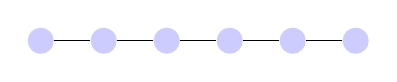
\begin{tikzpicture}
  [scale=.8,auto=left,every node/.style={circle,fill=blue!20}]
  \node (a) at (0,0) {};
  \node (b) at (1,0) {};
  \node (c) at (2,0) {};
  \node (d) at (3,0) {};
  \node (e) at (4,0) {};
  \node (f) at (5,0) {};
  \foreach \from/\to in {a/b,b/c,c/d,d/e,e/f}
    \draw (\from) -- (\to);
\end{tikzpicture}
\end{center}
To help with our proof, first we consider the following: \\

  Let $T$ be a \nameref{tree}. Let $n_i = $ number of vertices of \nameref{degree} $i$ in $T$ for $i \geq 0$. Assume $p = |V(T)| \geq 2$. So that $n_0 = 0$ (any vertex of \nameref{degree} 0 is in a \nameref{component} by itself). Also $n_i = 0$ for $i \geq p$ (next possible \nameref{degree} for a vertex is $p - 1$). \\

  Now we know that $|E(T)| = q = p - 1$, and
  \[ \sum_{v \in V(T)} \deg(v) = 2q \]
  we can rewrite this as
  \begin{align*}
    1n_1 + 2n_2 + 3n_3 + \cdots + (p-1)n_{p-1} & = 2(p-1) & (1) \\
    n_1 + n_2 + n_3 + \cdots + n_{p-1} & = p & (2)
  \end{align*}
  then $2\times$(2) - (1) is,
  \begin{align*}
      n_1 + 0 - n_3 - 2n_4 - 3n_5 - \cdots - (p-3)n_{p-1} & = 2 \\
      n_1 & = (n_3 + 2n_4 + 3n_5 + \cdots) + 2 & (\star)
   \end{align*}
   Now we start the proof since we have ($\star$)
   \begin{proof}
   From $(\star)$ we see that
   \[ n_1 \geq 2 \]
   so $T$ has at least 2 leaves.
\end{proof}
\begin{note}
  $n_2$ does not appear in $(\star)$.
\end{note}
\subsection{Spanning Trees}
\begin{defn}[spanning tree]\label{spanning tree}
  Let $G$ be a \nameref{graph}. A \textbf{spanning tree} in $G$ is a \nameref{spanning} \nameref{subgraph} that is also a \nameref{tree}.
\end{defn}
  \begin{center}$G$:
  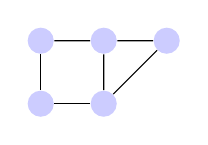
\begin{tikzpicture}
  [scale=.8,auto=left,every node/.style={circle,fill=blue!20}]
  \node (a) at (0,0) {};
  \node (b) at (1,0) {};
  \node (c) at (1,1) {};
  \node (d) at (0,1) {};
  \node (e) at (2,1) {};
  \foreach \from/\to in {a/b,b/c,c/d,d/a,b/e,e/c}
    \draw (\from) -- (\to);
\end{tikzpicture}
$H$:
  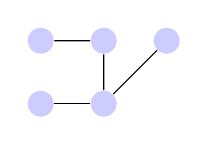
\begin{tikzpicture}
  [scale=.8,auto=left,every node/.style={circle,fill=blue!20}]
  \node (a) at (0,0) {};
  \node (b) at (1,0) {};
  \node (c) at (1,1) {};
  \node (d) at (0,1) {};
  \node (e) at (2,1) {};
  \foreach \from/\to in {a/b,b/c,c/d,b/e}
    \draw (\from) -- (\to);
\end{tikzpicture}
\end{center}
$H$ is a \nameref{spanning tree} of $G$.

\begin{thrm}
  A \nameref{graph} hs a \nameref{spanning tree} if and only if it is \nameref{connected}.
\end{thrm}
\begin{proof}
  ($\Longrightarrow$) Let $G$ be a \nameref{graph}, and let $T$ be a \nameref{spanning tree} of $G$. To prove $G$ is \nameref{connected}, take $x,y \in V(G)$. Since $T$ is a \nameref{tree} there is a \nameref{path} from $x$ to $y$ in $T$. This is also a \nameref{path} in $G$. Done. \\

  ($\Longleftarrow$) Let $G$ be a \nameref{connected} \nameref{graph}. If $G$ has no \nameref{cycle}s, then $G$ is a \nameref{tree}, and hence $G$ is a \nameref{spanning tree} of itself. If $G$ has a \nameref{cycle} let $e$ be an edge in a \nameref{cycle}. Consider $G - e$, since $e$ is in a \nameref{cycle}, $e$ is not a \nameref{bridge}. So, $G- e$ is \nameref{connected} and has fewer edges. Repeat until there are no \nameref{cycle}s left. The result must be a \nameref{connected} \nameref{spanning} \nameref{subgraph} with no \nameref{cycle}s, that is a \nameref{spanning tree}.
\end{proof}

\begin{cor}
  If $G$ is a \nameref{connected} \nameref{graph} with $p$ vertices and $q = p - 1$ edges, then $G$ is a \nameref{tree}.
\end{cor}

\begin{proof}
  Assume $G$ is \nameref{connected}. Then $G$ has a \nameref{spanning tree}, $T$. We know
  \[ V(T) = V(G) \]
  which means that \[
  |E(T)| = |V(T)| - 1 = p-1 = q\]
  but $|E(G)| = q$ which implies that $E(T) = E(G)$.
\end{proof}
\begin{note}
  \textbf{WARNING!} $G$ must be \nameref{connected}. Consider,
  \begin{center}
   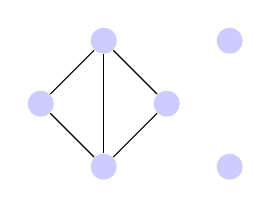
\begin{tikzpicture}
  [scale=.8,auto=left,every node/.style={circle,fill=blue!20}]
  \node (a) at (0,0) {};
  \node (b) at (1,1) {};
  \node (c) at (-1,1) {};
  \node (d) at (0,2) {};
  \node (e) at (2,0) {};
  \node (f) at (2,2) {};
  \foreach \from/\to in {a/b,b/d,c/d,d/a,a/c}
    \draw (\from) -- (\to);
\end{tikzpicture}
\end{center}
which has 6 vertices and 5 edges, but is not a \nameref{tree}.
\end{note}

\subsection{Breadth First Search Trees}

\textbf{Input.} A \nameref{graph} $G$ with $p$ vertices and a vertex $r \in V(G)$. \\

\textbf{Output.} A Breadth First Search Tree (BFST) \textbf{rooted} at $r$.

\begin{itemize}
  \item[1.] Begin $T$ with vertex $r$ ($r$ is called the \textbf{root} of $T$).
  \begin{itemize}
    \item Define $\ub{pr(r)}_{\mbox{parent}} = \phi \longleftarrow $ null
    \item Begin a queue of \textbf{unexhausted vertices} with $r$.
  \end{itemize}
  \item[2.] While the queue is non-empty do:
  \begin{itemize}
    \item Let $x$ be the vertex at the head of the queue ($x$ is called the \textbf{active vertex})
    \item While there is an edge $e = \{x,y\}$ where $y \not \in V(T)$.
    \begin{itemize}
      \item Add $y$ and $e$ to $T$
      \item define $pr(y) = x$
      \item Add $y$ to the queue
    \end{itemize}
    \item Delete $x$ from the queue
  \end{itemize}
  \item[3.] Output $(T, pr)$
\end{itemize}

\begin{exmp}
  Consider the graph,
  \begin{center}
   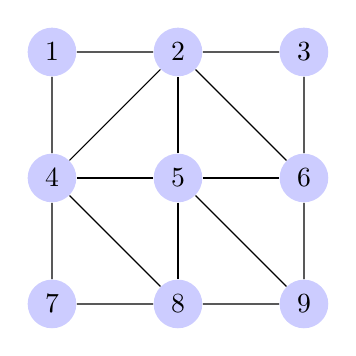
\begin{tikzpicture}
  [scale=.8,auto=left,every node/.style={circle,fill=blue!20}]
  \node (a) at (0,0) {5};
  \node (b) at (2,0) {6};
  \node (c) at (2,2) {3};
  \node (d) at (0,2) {2};
  \node (e) at (-2,2) {1};
  \node (f) at (-2,0) {4};
  \node (g) at (-2,-2) {7};
  \node (h) at (0,-2) {8};
  \node (i) at (2,-2) {9};
  \foreach \from/\to in {a/b,b/c,c/d,d/e,e/f,f/g,g/h,h/i,i/b,i/a,h/f,f/d,d/b,a/h,a/d,a/f,a/h}
    \draw (\from) -- (\to);
\end{tikzpicture}
\end{center}
\end{exmp}
Then the following Breadth First Search Tree is produced,
  \begin{center}
   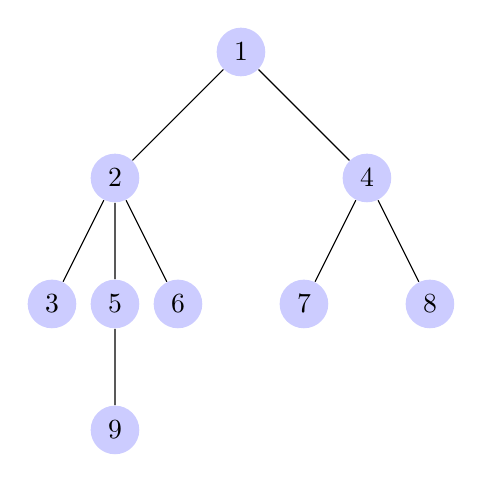
\begin{tikzpicture}
  [scale=.8,auto=left,every node/.style={circle,fill=blue!20}]
  \node (a) at (0,3) {1};
  \node (b) at (-2,1) {2};
  \node (c) at (2,1) {4};
  \node (d) at (-3,-1) {3};
  \node (e) at (-2,-1) {5};
  \node (f) at (-1,-1) {6};
  \node (g) at (-2,-3) {9};
  \node (h) at (1,-1) {7};
  \node (i) at (3,-1) {8};
  \foreach \from/\to in {a/b,a/c,b/d,b/e,b/f,e/g,c/h,c/i}
    \draw (\from) -- (\to);
\end{tikzpicture}
\end{center}
\begin{note}
  There may be choices. When there are multiple edges to add to an active vertex, the algorithm does not say what order to add them in.
\end{note}

\textbf{Applications of Breadth First Search Trees} \\

\begin{thrm}
  Let $G$ be a \nameref{graph} and let $T$ be a Breadth First Search Tree of $G$. That is, let $T$ be the output of this algorithm. \begin{itemize}
    \item[(i)]$T$ is always a \nameref{tree}
    \item[(ii)]$T$ is a \nameref{spanning tree} if and only if $G$ is \nameref{connected}.
  \end{itemize}
\end{thrm}

\begin{proof}
  \begin{itemize}
    \item[(i)] We will show that $T$ is \nameref{connected} and if $T$ has $k$ vertices, then $T$ has $k - 1$ edges.

    Note that for any vertex $v \in V(T)$, there is a \nameref{path}
    \[ v\ar pr(v) \ar pr(pr(v)) \ar \cdots pr^l(v) = r \]
    Therefore $T$ is \nameref{connected}. Also, $T$ begins with 1 vertex and 0 edges. In the algorithm, we always add 1 vertex and 1 edge together. Therefore, $|V(T)| = |E(T)| +1$ at all points in the algorithm. This shows that $T$ is a \nameref{tree}.
  \end{itemize}
  \item[(ii)] ($\Longrightarrow$) If $T$ is a \nameref{spanning tree} then $G$ is \nameref{connected}. \\
  ($\Longleftarrow$) If $T$ is not a \nameref{spanning tree}, then $V(T)$ is a proper non-empty subset of $V(G)$. The algorithm terminates when the \nameref{cut} on $V(T)$ is empty. Therefore $G$ is not \nameref{connected}.
\end{proof}
So the Breadth First Search Algorithm gives us a way to test whether \nameref{graph}s are \nameref{connected}.

Another application is a way of finding the distance between 2 vertices. Let $T$ be a Breadth First Search Tree rooted at $r$. For any $v \in V(T)$ there is a \nameref{path} which goes from $v$ to its parent, to its parent's parent and so forth until we reach the root,
\[ v\ar pr(v) \ar pr(pr(v)) \ar \cdots pr^l(v) = r \]
\begin{defn}[level]\label{level}
The \nameref{length} of this \nameref{path} is the \textbf{level}.
\end{defn}
For example, on the top of this page the tree drawn has 1 in level, 2 in level 2, 5 in level 3, and 1 in level 4. \\

\textbf{Fact.} In the breadth first search tree algorithm, the vertices of $T$ are added in non-decreasing order of \nameref{level}.

\begin{thrm}[Fundamental propert of BFSTs]\label{fundamentalbfst}
Let $G$ be a \nameref{connected} \nameref{graph}, and let $T$ be a Breadth First Search Tree of $G$. For any edge $e = \{x,y\} \in E(G)$, the vertices $x$ and $y$ are at most one \nameref{level} apart.
\end{thrm}

\begin{proof}
 Suppose without loss of generality that $i = level(x) \leq level(y)$. We show that $level(y) \leq i+1$. When $x$ becomes the active vertex in the breadth first search tree algorithm, there are two cases.
 \begin{itemize}
   \item[(1)] $y$ is already in the \nameref{tree}. Then $pr(y)$ must precede $x$ in the queue. (None of the vertices after $x$ have had their children added yet). Then $\level(pr(y)) \leq \level(x)$. Therefore $\level(y) = \level(pr(y)) + 1 \leq \level(x) + 1 = i + 1$.
   \item[(2)] $y$ is not already in the \nameref{tree}. Then $y$ gets added to the \nameref{tree} now, and $pr(y) = x$. Therefore $\level(y) = \level(x) + 1$.
 \end{itemize}
\end{proof}

\begin{defn}[distance]\label{distance}
The \textbf{distance} $d(u,v)$ between two vertices $u$ and $v$ in a \nameref{graph} $G$ is the \nameref{length} of a shortest \nameref{path} from $u$ to $v$.
\end{defn}

If there is no \nameref{path} from $u$ to $v$, $d(u,v)$ is undefined (or $d(u,v) = \infty$).

\begin{thrm}
  Let $G$ be a \nameref{connected} \nameref{graph} and let $u,v \in V(G)$. Let $T$ be a breadth first search tree rooted at $u$. Then, $d(u,v) = \level(v)$.
\end{thrm}

\begin{proof}
  We'll prove two things:
  \begin{itemize}
    \item[(1)] $d(u,v) \geq \level(v)$
    \item[(2)] $d(u,v) \leq \level(v)$
  \end{itemize}
  So,
  \begin{itemize}
    \item[(1)] Consider a shortest \nameref{path} from $u$ to $v$:
    \[ u = x_0x_1x_2\cdots x_k = v\]
    We know that $\level(v) = \level(x_k) \leq \level(x_{k-1}) + 1$ by \nameref{fundamentalbfst}, we can repeat this so,
    \begin{align*}
      \level(x_k) & \leq \level(x_{k-1}) + 1 \\
                  & \leq \level(x_{k-2}) + 2 \\
                  & \vdots \\
                  & \leq \level(x_0) + k \\
                  & = k & \mbox{(since $u = x_0$ is the root)}
                  & = d(u,v)
    \end{align*}
    Then we have shown that $d(u,v) \geq \level(v)$.
    \item[(2)] Note that $v, pr(v), pr^2(v), \ldots, pr^k(v) = u$ is a \nameref{path} from $u$ to $v$ whose \nameref{distance} is $\level(v)$. Either this is a shortest \nameref{path}, or there's a shorter one. Therefore, $\level(v) \geq d(u,v)$.
  \end{itemize}
\end{proof}
This proves that
\[ v, pr(v), pr^2(v), \ldots, pr^k(v) = u \]
is a shortest \nameref{path} from $u$ to $v$ if $u$ is the root. There be other shortest \nameref{path}s. \\
\textbf{WARNING!} This only works if one of the two vertices involved is the root of $T$.

Another way that the algorithm helps, is finding \nameref{bipartite} \nameref{graph}s.

\begin{thrm}
  Let $G$ be a \nameref{connected} \nameref{graph}. Then the following are equivalent.
  \begin{itemize}
    \item[i.] $G$ is \nameref{bipartite}
    \item[ii.] $G$ has no odd \nameref{cycle}s
    \item[iii.] Let $T$ be a breadth first search tree of $G$. There are no edges of $G$ joining two vertices of the same \nameref{level}.
  \end{itemize}
\end{thrm}
\begin{proof}
  We will prove that (1) $i. \implies ii.$ and (2) $ii. \implies iii.$ and (3) $iii. \implies i.$. We have already shown $i. \implies ii.$.
  \begin{itemize}
    \item[(2)] In contrapositive form: If there is an edge, $\{x,y\} \in E(G)$ such that $\level(x) = \level(y)$, then $G$ has an odd \nameref{cycle}. Consider the \nameref{subgraph} formed by the edge $e=\{x,y\}$ and the \nameref{path} \[ x, pr(x),pr^2(x),\ldots,pr^t(x) \]
    \[ y,pr(y),\ldots,pr^t(y) \]
    where $pr^t(x) = pr^t(y)$ is the first common ancestor of $x$ and $y$. This is a \nameref{cycle} of \nameref{length} $2t+1$.
    \item[(3)] Let $A = \{v\in V(G) \ | \ \level(v) \mbox{\ is odd} \}$ and $B = \{v \in V(G) \ | \ \level(v) \mbox{\ is even}\}$. Since there are no edges of $G$ joining two vertices of the same \nameref{level}, every pair of adjacent vertices is exactly one \nameref{level} apart. That means, one is in $A$ and one is $B$, therefore $(A,B)$ is a bipartition, therefore the \nameref{graph} $G$ is \nameref{bipartite}.
  \end{itemize}
\end{proof}

\subsection{Planar Graphs}

\begin{defn}[planar]\label{planar}
A \nameref{graph} is \textbf{planar} if it can be drawn in the plane with no edges crossing.
\end{defn}

For example,
\begin{center}$O_3$
  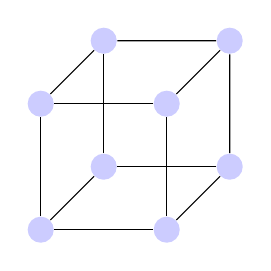
\begin{tikzpicture}
  [scale=.8,auto=left,every node/.style={circle,fill=blue!20}]
  \node (na) at (2,4) {};
  \node (nb) at (4,4)  {};
  \node (nc) at (1,3) {};
  \node (nd) at (3,3) {};
  \node (ne) at (1,1) {};
  \node (nf) at (3,1)  {};
  \node (ng) at (4,2) {};
  \node (nh) at (2,2) {};
  \foreach \from/\to in {nh/na,na/nb,na/nc,ne/nh,ne/nf,nf/ng,nd/nb,nd/nc,nd/nf,ne/nc,ng/nb,ng/nh}
    \draw (\from) -- (\to);
\end{tikzpicture}
\end{center}
is planar, redrawn it looks like:
\begin{center}$O_3$
  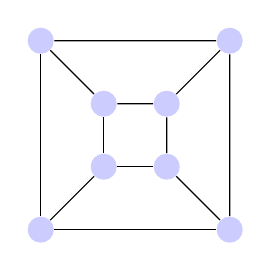
\begin{tikzpicture}
  [scale=.8,auto=left,every node/.style={circle,fill=blue!20}]
  \node (na) at (0,1) {};
  \node (nb) at (0,0)  {};
  \node (nc) at (1,0) {};
  \node (nd) at (1,1) {};
  \node (ne) at (-1,2) {};
  \node (nf) at (-1,-1)  {};
  \node (ng) at (2,-1) {};
  \node (nh) at (2,2) {};
  \foreach \from/\to in {na/nb,nb/nc,nc/nd,nd/na, na/ne,nb/nf,nc/ng,nd/nh,ne/nf,nf/ng,ng/nh,nh/ne}
    \draw (\from) -- (\to);
\end{tikzpicture}
\end{center}

Some other planar graphs include $K_5$. $K_5$ is not planar (try it). $K_{3,3}$ is also not planar. So how do we prove this?

\begin{note}
  A \nameref{graph} is \nameref{planar} if and only if all of its \nameref{component}s are \nameref{planar}.
\end{note}

\begin{defn}[planar embedding]\label{planar embedding}
A \textbf{planar embedding} is a specific drawing of a \nameref{graph} in the plane with no edges crossing.
\end{defn}

\begin{defn}[face]\label{face}
A \nameref{planar embedding} divides the plane into regions called \textbf{faces}.
\end{defn}
  \begin{defn}[adjacent]\label{adjacent}
  Two faces are \textbf{adjacent} if they are \textbf{incident} with a common edge.
  \end{defn}
  \begin{defn}[boundary]\label{boundary}
  The \textbf{boundary} of a face is the \nameref{subgraph} consisting of all vertices and edges incident with the face.
  \end{defn}
  \begin{defn}[degree]\label{pdegree}
  The \textbf{degree} of a face is the number of edges in the boundary with \nameref{bridge}s counted twice.
  \end{defn}

  \begin{exmp}
    Some examples,
    \begin{center}
  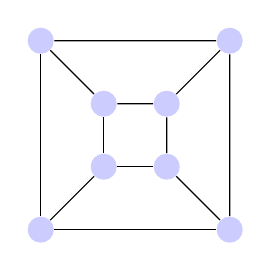
\begin{tikzpicture}
  [scale=.8,auto=left,every node/.style={circle,fill=blue!20}]
  \node (na) at (0,1) {};
  \node (nb) at (0,0)  {};
  \node (nc) at (1,0) {};
  \node (nd) at (1,1) {};
  \node (ne) at (-1,2) {};
  \node (nf) at (-1,-1)  {};
  \node (ng) at (2,-1) {};
  \node (nh) at (2,2) {};
  \foreach \from/\to in {na/nb,nb/nc,nc/nd,nd/na, na/ne,nb/nf,nc/ng,nd/nh,ne/nf,nf/ng,ng/nh,nh/ne}
    \draw (\from) -- (\to);
\end{tikzpicture}
\end{center}
Each empty space within this figure is a face, and the empty space outside of it is also a face. So there are $p = 8$ vertices, $q = 12$ edges, $s = 6$ faces. Aditionally, for each face $f_i$ from $1 \leq i \leq 6$, $\deg(f_i) = 4$. For the graph
\begin{center}
  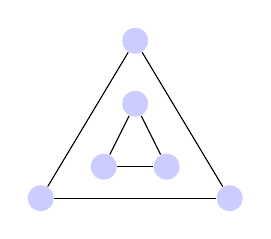
\begin{tikzpicture}
  [scale=.8,auto=left,every node/.style={circle,fill=blue!20}]
  \node (na) at (0,0) {};
  \node (nb) at (1,0)  {};
  \node (nc) at (0.5,1) {};
  \node (nd) at (-1,-0.5) {};
  \node (ne) at (0.5, 2) {};
  \node (nf) at (2,-0.5)  {};
  \foreach \from/\to in {na/nb,nb/nc,nc/na, nd/ne,ne/nf,nf/nd}
    \draw (\from) -- (\to);
\end{tikzpicture}
\end{center}
has 6 vertices, 6 edges, and 3 faces. The degree of the face in the inner triangle is 3, of the face between the boundaries of both triangles is 6, and the degree of the face of the outside is 3.
  \end{exmp}
also,
  \begin{center}
  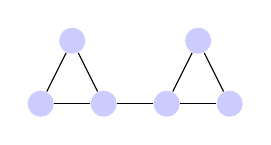
\begin{tikzpicture}
  [scale=.8,auto=left,every node/.style={circle,fill=blue!20}]
  \node (na) at (0,0) {};
  \node (nb) at (1,0)  {};
  \node (nc) at (0.5,1) {};
  \node (nd) at (2,0) {};
  \node (ne) at (3,0) {};
  \node (nf) at (2.5,1)  {};
  \foreach \from/\to in {na/nb,nb/nc,nc/na, nd/ne,ne/nf,nf/nd,nb/nd}
    \draw (\from) -- (\to);
\end{tikzpicture}
\end{center}
then there are 6 vertices, 7 edges, and 3 faces. The degree of the face of the left triangle is 3, the degree of the face in the right triangle is 3, and the degree of the outside face is 8. \\

\textbf{Key Observation.} In a \nameref{planar embedding},
\begin{itemize}
  \item a \nameref{bridge} is incident with just one \nameref{face}
  \item a non-\nameref{bridge} is incident with two different \nameref{face}s.
\end{itemize}

\begin{thrm}
  For a \nameref{planar embedding} with $q$ edges and faces $f_1,f_2,\ldots,f_s$, then
  \[ \sum_{i = 1}^s \deg(f_i) = 2q\]
\end{thrm}
\begin{proof}
  Each edge that is not a \nameref{bridge} is incident with 2 \nameref{face}s, so gets counted twice on the LHS. Each \nameref{bridge} is incident with one \nameref{face}, but gets counted twice in the \nameref{pdegree} of that \nameref{face}. Therefore the LHS counts each edge twice.
\end{proof}

A \nameref{graph} can have different \nameref{planar embedding}s. For example, both of these graphs are equal

\begin{center}
   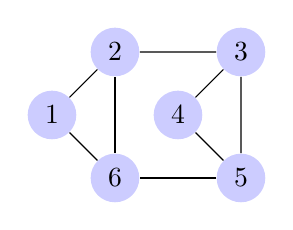
\begin{tikzpicture}
  [scale=.8,auto=left,every node/.style={circle,fill=blue!20}]
  \node (a) at (0,0) {6};
  \node (b) at (1,1) {4};
  \node (c) at (-1,1) {1};
  \node (d) at (0,2) {2};
  \node (e) at (2,0) {5};
  \node (f) at (2,2) {3};
  \foreach \from/\to in {c/d,d/a,a/c,f/e,f/d,e/a,e/b,f/b}
    \draw (\from) -- (\to);
\end{tikzpicture}
 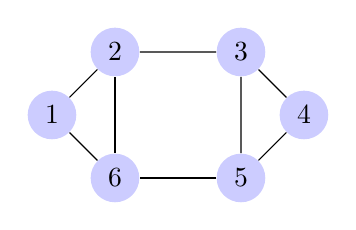
\begin{tikzpicture}
  [scale=.8,auto=left,every node/.style={circle,fill=blue!20}]
  \node (a) at (0,0) {6};
  \node (b) at (3,1) {4};
  \node (c) at (-1,1) {1};
  \node (d) at (0,2) {2};
  \node (e) at (2,0) {5};
  \node (f) at (2,2) {3};
  \foreach \from/\to in {c/d,d/a,a/c,f/e,f/d,e/a,e/b,f/b}
    \draw (\from) -- (\to);
\end{tikzpicture}
\end{center}

Their face degree sequences are (respectively), $5,5,3,3$ and $6,4,3,3$. Not a feature of \nameref{graph} itself.

\begin{thrm}[Euler's Formula]\label{eulers}
  For a \nameref{planar embedding} with $p$ vertices, $q$ edges, $s$ faces and $c$ components, then
  \[ p - q + s = c + 1 \]
\end{thrm}

\begin{cor}
  For a \nameref{connected} \nameref{planar embedding} with $p$ vertices, $q$ edges, and $s$ faces then
  \[ p - q + s = 2 \]
\end{cor}

\begin{proof}
  By induction on $q$, the number of edges. \\

  \textbf{Base Case.} Prove it for all \nameref{planar} \nameref{graph}s with $q = 0$ edges. If there are $p$ vertices, then $c = p$ and $s = 1$. Check $p - q + s = p - 1$ and $c + 1 = p + 1$. Thus, $p - q + s = c + 1$. \\

  \textbf{Inductive Hypothesis.} Fix $p > 0$ and assume \nameref{eulers} holds for \nameref{graph}s with $q - 1$ edges. \\

  \textbf{Inductive Step.} Let $P$ be a \nameref{planar embedding} with $p$ vertices, $q$ edges, $s$ \nameref{face}s, and $c$ \nameref{component}s. Let $e$ be an edge of $P$ and consider $P - e$. $P-e$ has $p$ vertices, $q' = q - 1$ edges, $s'$ \nameref{face}s, and $c'$ \nameref{component}s. By the inductive hypothesis, $p' - q' + s' = c' + 1$.
  \begin{itemize}
    \item \textbf{Case 1}. If $e$ is a \nameref{bridge}, then $c' = c + 1$ (Lemma 4.1). Also $e$ is incident with only one \nameref{face} (the face on one side of $e$ is the same face as the face on the other side). So when we delete $e$, we do not create any new faces. Therefore $s' = s$. This implies that $p - (q-1) + s = (c+1) + 1$, and therefore $p - 1 + s = c + 1$.
    \item \textbf{Case 2}. If $e$ is not a bridge, then $c' = c$ (by definition). Also $e$ is incident with 2 different faces, when we delete $e$, these become 1 face, and therefore $s' = s - 1$. Then $p - (q - 1) + (s - 1) = c + 1$ which implies $p - q + s = c + 1$.
  \end{itemize}
\end{proof}
The proof in the course notes is fairly similar, but the case base is a \nameref{tree}, with $p$ vertices, $p - 1$ edges, and 1 face. How do we know there's only 1 face though? This proof also skips case 1, because the \nameref{graph} is \nameref{connected}. To prove a \nameref{tree} has one face is to prove it using induction using the argument in case 1.

\subsection{Platonic Solids}

In Platonic Solids,
\begin{itemize}
  \item Faces are regular polygons.
  \item There are the same number of faces meeting at every vertex. ($d$ faces at each vertex)
  \item Can be modeled by a \nameref{planar graph}.
\end{itemize}

Then let $d^*$ be the \nameref{pdegree} of every face, and then $d$ the \nameref{pdegree} of every vertex. If we want to study Platonic Solids, we should study \nameref{connected} \nameref{planar graph}s, where every \nameref{face} has \nameref{pdegree} $d^*$ and every vertex has \nameref{pdegree} $d$. \\

We have three equations: ($p$ vertices, $q$ edges, $s$ faces)
\begin{align*}
  \sum_{v \in V(G)} \deg(v) & = 2q \implies pd = 2q &(1) \\
  \sum_{i = 1}^s \deg(f_i) & = 2q \implies sd^* = 2q &(2) \\
  p + q - s & = 2 &(3)
\end{align*}

\textbf{Question.} What are the possible values of $d$ and $d^*$?

We solve the system of equations, first by eliminating $p$ and $s$.
\[ p = \f{2q}{d} \ \ \ \ \ \ \ \ \ \ s = \f{2q}{d^*} \]
Then Euler's formula becomes,
\[ \f{2q}{d} - q + \f{2q}{d^*} = 2 \]
Move all the $q$'s to one side
\[ \f{2q}{d} + \f{2q}{d^*} = \f{2+q}{q} \]
since $\f{2+q}{q} > 1$, we have
\[ \f{2}{d} + \f{2}{d^*} > 1 \]
Multiply by $dd^*$ to get
\begin{align*}
   2d^* + 2d & > dd^* \\
   dd^* - 2d^* - 2d & < 0 \\
   dd^* -2d^* -2d + 4 & < 4 \\
   (d - 2)(d^* - 2) & < 4
 \end{align*}
 The possibilities are $d = 2$, which is some $d^*$-cycle, or $d > 2$ (to get a 3-dimensional object), in which case $(d, d^*) \in \{(3,3), (4,3), (3,4), (5,3), (3,5)\}$. These pairs correspond to the 5 platonic solids.
 \begin{itemize}
   \item $(3,4)$ is the cube
   \item $(4,3)$ is the octahedron
   \item $(3,3)$ is the tetrahedron
   \item $(5,3)$ is the icosahedron
   \item $(3,5)$ is the dodecahedron
 \end{itemize}

 The next goal is to prove that $K_5$ is \textbf{not} \nameref{planar}.
 \begin{itemize}
   \item Assume it is
   \item Use these equations
   \item Get a contradiction
 \end{itemize}

 In order to do this we need a general property about faces of \nameref{planar} \nameref{graph}s.

 \begin{defn}[girth]\label{girth}
 If $G$ is a \nameref{graph} with a \nameref{cycle}, the \textbf{girth} of $G$ is the \nameref{length} of a shortest \nameref{cycle}. For example, the following graph has girth 4.
 \begin{center}
  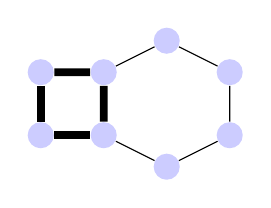
\begin{tikzpicture}
  [scale=.8,auto=left,every node/.style={circle,fill=blue!20}]
  \node (a) at (0,0) {};
  \node (b) at (1,0) {};
  \node (c) at (1,1) {};
  \node (d) at (0,1) {};
  \node (e) at (2,1.5) {};
  \node (f) at (3,1) {};
  \node (g) at (3,0) {};
  \node (h) at (2,-0.5) {};
  \foreach \from/\to in {a/b,b/c,c/d,d/a}
    \draw [line width=1mm] (\from) -- (\to);
    \foreach \from/\to in {c/e,e/f,f/g,g/h,h/b}
    \draw  (\from) -- (\to);
\end{tikzpicture}
\end{center}
 \end{defn}

 \begin{thrm}
   $K_5$ is not \nameref{planar}.
 \end{thrm}

 \begin{proof}
   Suppose it were \nameref{planar}. Then we would have a \nameref{planar embedding} with $p = 5$vertices, $q = 10$ edges, $s$ faces, and every \nameref{face} has \nameref{pdegree} greater than or equal to 3. Thus $\girth(K_5) = 3$. By \nameref{eulers},
   \[ s = q - p + 2 = 7 \]
   Let $f_1, f_2, \ldots, f_7$ be the \nameref{face}s. Then
   \[ \sum_{i = 1}^s \deg(f_i) = 20 \]
   but $\deg(f_i) \leq 3$ for $1 \leq i \leq 7$, so $\sum \deg(f_i) \geq 21$. This is a contradiction.
 \end{proof}

 \begin{thrm}
   $K_{3,3}$ is not \nameref{planar}.
 \end{thrm}

 \begin{proof}
   Suppose it were. Then we would have a \nameref{planar embedding} with $p = 6$, $q = 9$ and $s$ faces. By \nameref{eulers}, $s = q - p + 2 = 5$. Let $f_1, \ldots, f_5$ be the faces, then since $\girth(K_{3,3}) = 4$,  $\deg(f_i) \geq 4$. However,
   \[ \sum \deg (f_i) = 2q = 18 \]
   \[ \sum \deg (f_i) \geq 4s = 20 \]
   contradiction.
 \end{proof}

 \textbf{Exerciese:} Prove that the Petersen graph is not planar.

 \begin{note}
   You cannot use this method to prove that a \nameref{graph} is \nameref{planar}.
 \end{note}

  \begin{thrm}
   Let $G$ be a \nameref{graph} with a \nameref{cycle}. Suppose $\girth(G) = k$. If a \nameref{planar embedding} of $G$ exists, then every \nameref{face} of that \nameref{planar embedding} has \nameref{pdegree} at least $k$.
 \end{thrm}

 In the next little bit we will

 \begin{itemize}
   \item Prove this theorem
   \item Streamline the method (new equation)
   \item What to do if this method doesn't work
   \item Applications to graph colouring
 \end{itemize}

 \begin{lem}
   Let $P$ be a \nameref{planar embedding} of a \nameref{graph} with a \nameref{cycle}. Then the boundary of every \nameref{face} of $P$ also has a \nameref{cycle}.
 \end{lem}

 \begin{proof}
   Let $f$ be a \nameref{face} of $P$. Let $H$ be the \nameref{boundary} of $f$. $H$ is a \nameref{subgraph} of $P$ embedded in the plane and $f$ is also a \nameref{face} of $H$. Since $P$ contains a \nameref{cycle}, there is an edge of $P$ that is not an edge. This edge is incident with 2 \nameref{face}s.
   \begin{itemize}
     \item Therefore $P$ has at least 2 faces.
     \item Therefore $f$ is not the whole plane.
     \item Therefore $H$ has another face.
   \end{itemize}
   Therefore there is an edge along which two faces are adjacent. This edge cannot be a \nameref{bridge} which implies that $H$ is a \nameref{cycle}.
 \end{proof}

 \begin{proof}[Prooof of Theorem 4.20]
   Let $P$ be a \nameref{planar embedding} of $G$ and let $f$ be a \nameref{face}. By the lemma, the \nameref{boundary} of $f$ has a \nameref{cycle} $C$. Then
   \[ k \leq length(C) \leq \mbox{the number of edges in the boundary of $f$} \leq \deg(f) \]
 \end{proof}

 \begin{thrm}
   Suppose $G$ is a \nameref{planar embedding} with $p$ vertices, $q$ edges, and suppose every \nameref{face} has \nameref{pdegree} at least $d^* \geq 3$. Then,
   \[ q \le \f{d^*(p-2)}{d^* - 2} \]
 \end{thrm}
 \begin{proof}
   Let $'f_1, f_2, \ldots, f_s'$ be the \nameref{face}s of $G$.
   \[ 2q = \sum_{i = 1}^2\deg(f_i) \geq d^* s \implies s \leq \f{2q}{d^*} \]
   By \nameref{eulers},
   \[ p - q + s = c + 1 \ \ \ \ \ \ \ \ \ \mbox{where $c$ is the number of \nameref{component}s} \]
   Since $c \geq 1$, $p - q + s \geq 2$,
   \begin{align*}
     s & \geq 2 + q - p \\
     \implies 2d^* + qd^* - pd^* & \leq 2q \\
     \implies 2q - qd^* &\geq 2d^* - pd^* \\
     \implies (2-d^*)q &\geq d^*(2-p) \\
     \implies q &\leq \f{d^*(2-p)}{2-d^*} \\
     \implies q & \leq \f{d^*(p-2)}{d^* - 2}
   \end{align*}
 \end{proof}

 \textbf{Applications.} In any \nameref{planar graph} with $p \geq 3$ vertices and $q$ edges, we have
 \[ q \leq 3p - 6 \]
 This is the maximum possible number of edges in a \nameref{planar graph}.
 \begin{proof}
   If $G$ has a \nameref{cycle}, then by Lemma 4.2, every \nameref{face} $f_i$ of a \nameref{planar embedding} of $G$ has $\deg(f_i) \geq \girth(G) \geq 3$. Therefore by Theorem 4.21 with $d^* = 3$ implies
   \[ q \leq \f{3(p-2)}{3-2} = 3p - 6 \]
   Otherwise, if $G$ does not have a \nameref{cycle}, then $G$ is a forest (every \nameref{component} is a \nameref{tree}), therefore
   \[ q \leq p - 1 \leq 3p - 6 \]
 \end{proof}
 \begin{exmp}
    Use this to show that $K_5$ is not \nameref{planar}. \\

    For $K_5$, $p = 5$ and $q = 10$. Is $q \leq 3p - 6$? No. Therefore $K_5$ is not \nameref{planar}.
  \end{exmp}

  Note that this doesn't work for $K_{3,3}$. In this case we have $p = 6$ and $q = 9$, but $q \leq 3p - 6$ is a valid inequality so we have no conclusion.\\

  \textbf{Application 2.} Suppose $G$ is a \nameref{graph} with a \nameref{cycle}, and $\girth(G) \geq k$. If $G$ is \nameref{planar} then
  \[ q \leq \f{k(p-2)}{k-2} \]

  \begin{proof}
    We know that every \nameref{face} of a \nameref{planar embedding} of $G$ has \nameref{pdegree} greater than or equal to $k$.
  \end{proof}

  Main Point: The \nameref{girth} of $G$ is always an acceptable value for $d^*$.

  \begin{exmp}
    Prove $K_{3,3}$ is not \nameref{planar} ($p = 6, q = 9, k = \girth(K_{3,3}) = 4$). Is it true that
    \[ q \leq \f{k(p-2)}{k-2} \]
    No. $LHS = 9$, and $RHS = 8$. So, $K_{3,3}$ is not \nameref{planar}.
  \end{exmp}

  \begin{exmp}
    Consider
        \begin{center}
  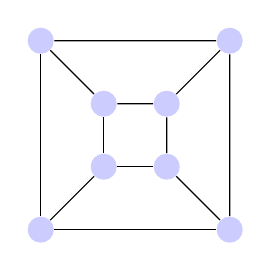
\begin{tikzpicture}
  [scale=.8,auto=left,every node/.style={circle,fill=blue!20}]
  \node (na) at (0,1) {};
  \node (nb) at (0,0)  {};
  \node (nc) at (1,0) {};
  \node (nd) at (1,1) {};
  \node (ne) at (-1,2) {};
  \node (nf) at (-1,-1)  {};
  \node (ng) at (2,-1) {};
  \node (nh) at (2,2) {};
  \foreach \from/\to in {na/nb,nb/nc,nc/nd,nd/na, na/ne,nb/nf,nc/ng,nd/nh,ne/nf,nf/ng,ng/nh,nh/ne}
    \draw (\from) -- (\to);
\end{tikzpicture}
\end{center}
then redrawn as
    \begin{center}
  \begin{tikzpicture}
  [scale=.8,auto=left,every node/.style={circle,fill=blue!20}]
  \node (na) at (0,1) {};
  \node (nb) at (0,0)  {};
  \node (nc) at (1,0) {};
  \node (nd) at (1,1) {};
  \node (ne) at (-1,2) {};
  \node (nf) at (-1,-1)  {};
  \node (ng) at (2,-1) {};
  \node (nh) at (2,2) {};
  \draw  (ne) to [out=200,in=200] (ng);
  \draw  (nh) to [out=0,in=-45] (nf);
  \foreach \from/\to in {na/nb,nb/nc,nc/nd,nd/na,na/ne,nb/nf,nc/ng,nd/nh,nf/ng,nh/ne}
    \draw (\from) -- (\to);
\end{tikzpicture}
\end{center}
This has the same $p = 8$, $q = 12$, and girth $k = 4$. However, it is not planar.
  \end{exmp}

\begin{exmp}
  Consider
  \begin{center}
  \begin{tikzpicture}
  [scale=.8,auto=left,every node/.style={circle,fill=blue!20}]
  \node (na) at (0,1) {};
  \node (nb) at (1,0)  {};
  \node (nc) at (-1,0)  {};
  \node (nd) at (-0.5,-1) {};
  \node (ne) at (0.5,-1)  {};
  \node (a) at (2, 0) {};
   \node (b) at (3, 0) {};
    \node (c) at (4, 0) {};
     \node (d) at (5, 0) {};
  \foreach \from/\to in {na/nb,na/ne,na/nd,na/nc,nb/nd,nb/nc,ne/nc,nd/ne,nd/nc, nb/ne, nb/a, a/b, b/c, c/d}
    \draw (\from) -- (\to);
\end{tikzpicture}
\end{center}
with $p = 2$, $q = 17$ and $k = 3$. And
\[ q \leq \f{k(p-2)}{k-2} \]
has $LHS = 17$, $RHS = 30$. By adding stuff to a non-\nameref{planar} \nameref{graph}, the equation $q \leq \f{k(p-2)}{k-2}$ might become satisfied.
\end{exmp}

\begin{defn}[edge subdivision]\label{edge subdivision}
An edge subdivision of a \nameref{graph} $G$ is obtained by applying the following operation, independently, to each edge of $G$: replace the edge by a path of length 1 or more; if the path has length $m > 1$, then there are $m - 1$ new vertices and $m - 1$ new edges created; if the path has length $m = 1$, then the edge is unchanged.
\end{defn}

\begin{thrm}[Kuratowski's Theorem]\label{kuratowski}
A \nameref{graph} is non-\nameref{planar} if and only if it has a \nameref{subgraph} that is either an edge-subdivision of $K_{3,3}$ or an edge-subdivision of $K_5$.
\end{thrm}

\begin{proof}
  CO 342
\end{proof}

The best way to determine if a \nameref{graph} is \nameref{planar}:

\begin{itemize}
  \item First, make a guess about whether or not it is \nameref{planar}
  \begin{itemize}
    \item[(a)] If yes, rewdraw it without crossings. Check out this website: \url{planarity.net}
    \item[(b)] If not, count the vertices $p$ and edges $q$, is $q > 3p - 6$?
    \begin{itemize}
      \item[i.] If yes, conclude that the \nameref{graph} is not \nameref{planar}.
      \item[ii.] If not, let $k$ be the girth of the \nameref{graph}; is $q > \f{k(p-2)}{k-2}$?
      \begin{itemize}
        \item If yes, then conclude the \nameref{graph} is not \nameref{planar}.
        \item If not, find an edge-subdivision $K_5$ or $K_{3,3}$. Do this by identifying that it might be an edge-subdivision of $K_{5}$, since that one is more likely, and then note that there \textbf{must} be five distinct vertices that have degree 5.
      \end{itemize}
    \end{itemize}
  \end{itemize}
\end{itemize}

\subsection{Graph Colouring}

\begin{defn}[$k$-colouring]\label{k-colouring}
A \textbf{$k$-colouring} of a \nameref{graph} $G$ is an assignment of $k$ (or fewer) colours to the vertices of $G$, such that no pair of adjacent vertices has the same colour. If a $k$-colouring exists, we say the \nameref{graph} is $k$-colourable.
\end{defn}

\begin{exmp}
Find a 3-colouring of the petersen graph:
   \begin{center}
  \begin{tikzpicture}
  [scale=.8,auto=left,every node/.style={circle,fill=blue!20}]
  \node (na) at (0,1) {2};
  \node (nb) at (1,0)  {3};
  \node (ne) at (-1,0)  {1};
  \node (nd) at (-0.5,-1) {1};
  \node (nc) at (0.5,-1)  {3};
  \node (nA) at (0,2) {1};
  \node (nB) at (2,0)  {2};
  \node (nE) at (-2,0)  {3};
  \node (nD) at (-1.5,-2) {2};
  \node (nC) at (1.5,-2)  {1};
    \foreach \from/\to in {nA/nB,nB/nC,nC/nD,nD/nE,nA/na,nB/nb,nC/nc,nD/nd,nE/ne,na/nc,nb/ne,nc/ne,nd/na,nE/nA, nd/nb}
    \draw (\from) -- (\to);
  \end{tikzpicture}
  \end{center}
  This means that the Petersen \nameref{graph} is 3-colourable. Is it 4-colourable? Yes. Is it 2-colourable? No.
\end{exmp}

\begin{note}
  2-colourable is the same thing as \nameref{bipartite}. If a bipartition is bipartite with $A$ and $B$ then vertices in $A$ get colour 1 and in $B$ they get colour 2.
\end{note}

The 2-colourable is easy because there is an efficient algorithm. 3-colourable is a totally different story, it is hard, and there is no efficient algorithm.

\begin{thrm}[4 colour theorem]\label{4color}
  Every \nameref{planar} \nameref{graph} is 4-colourable.
\end{thrm}

\begin{proof}
  The proof is not human-readable. Check this out: \url{http://research.microsoft.com/en-us/um/people/gonthier/4colproof.pdf}.
\end{proof}

\begin{thrm}[6-colour theorem]\label{6color}
  Every \nameref{planar} \nameref{graph} is 6-colourable.
\end{thrm}

\begin{lem}
  Every \nameref{planar} \nameref{graph} has a vertex $v$ with $\deg(v) \leq 5$.
\end{lem}

\begin{proof}
  Suppose to the contrary that $G$ is a \nameref{planar} \nameref{graph} with $p$ vertices and $q$ edges, and $\deg(v) \geq 6$ for all $v \in V(G)$. This means that
 \[ 2q = \sum_{v \in V(G)} \deg(v) \geq 6p \]
 which implies $q \geq 3p$. But since $G$ is \nameref{planar}, $q \leq 3p - 6$.
\end{proof}

\begin{proof}[Proof of 6-colour theorem]
  By induction on the number of vertices $p$. \\

  \textbf{Base Case.} A \nameref{graph} with 1 vertex is 6-colourable. \\

  \textbf{Inductive Hypothesis.} Let $p \geq 2$ and assume that every \nameref{planar graph} with $p - 1$ vertices is 6-colourable. \\

  \textbf{Inductive Step.} Let $G$ be a \nameref{planar graph} with $p$ vertices. Choose a vertex $v \in V(G)$ such that $\deg(v) \leq 5$. (possible, by Lemma 4.3). Let $G - v$ be the \nameref{subgraph} of $G$ with vertex set $V(G) \setminus \{v\}$ and all edges of $G$ that are not incident with $v$. For example,
  \begin{center}$G$
  \begin{tikzpicture}
  [scale=.8,auto=left,every node/.style={circle,fill=blue!20}]
  \node (na) at (0.5,1) {};
  \node (nb) at (-0.5,1) {};
  \node (nc) at (1,0)  {};
  \node (nd) at (-1,0)  {};
  \node (ne) at (-0.5,-1) {};
  \node (nf) at (0.5,-1)  {};
  \node (v) at (0, 0) {$v$};
    \foreach \from/\to in {na/nc,nc/nf,nf/ne,ne/nd,nd/nb,nb/na,nd/v,nc/v}
    \draw (\from) -- (\to);
  \end{tikzpicture}$G-v$
  \begin{tikzpicture}
  [scale=.8,auto=left,every node/.style={circle,fill=blue!20}]
  \node (na) at (0.5,1) {};
  \node (nb) at (-0.5,1) {};
  \node (nc) at (1,0)  {};
  \node (nd) at (-1,0)  {};
  \node (ne) at (-0.5,-1) {};
  \node (nf) at (0.5,-1)  {};
    \foreach \from/\to in {na/nc,nc/nf,nf/ne,ne/nd,nd/nb,nb/na}
    \draw (\from) -- (\to);
\end{tikzpicture}
\end{center}
Since $G - v$ is a \nameref{subgraph} of a \nameref{planar graph}, $G - v$ is \nameref{planar}, and it has $p - 1$ vertices. By the inductive hypothesis $G-v$ has a 6-colouring. We can extend this to a 6-colouring of $G$, by assigning $v$ one the colours not used by its neighbours. ($v$ has at most 5 neighbours, so there's a colour left.). Therefore $G$ is 6-colourable as required.
\end{proof}

\begin{thrm}[5-colour theorem]\label{5colour}
Every \nameref{planar graph} is 5-colourable.
\end{thrm}

\begin{proof}
  Basically the same as the 6-colour theorem. But here's a case where that proof doesn't work. If $v$ has 5 neighbours, and all have different colours, we're stuck.

  \begin{note}
    The neighbours of $v$ can't all be adjacent to each other; there must be two neighbours of $v$, say $x$ and $y$ that are not adjacent in $G$. (why? if they were all adjcent, the nighbours of $v$ would form a $K_5$-subgraph, which can't appear in a \nameref{planar graph}).
  \end{note}

\begin{center}
  \begin{tikzpicture}
  [scale=.8,auto=left,every node/.style={circle,fill=blue!20}]
  \node (na) at (0,1) {$y$};
  \node (nb) at (1,0)  {$b$};
  \node (nc) at (0.5,-1)  {$c$};
  \node (nd) at (-0.5,-1) {$x$};
  \node (ne) at (-1,0)  {$a$};
  \node (v) at (0,0) {$v$};
  \draw  (ne) to [out=200,in=250,distance=2cm] (nc);
  \draw  (ne) to [out=90,in=90,distance=2cm] (nb);
  \foreach \from/\to in {na/nb,nb/nc,nc/nd,nd/ne,ne/na,na/v,nb/v,nc/v,nd/v,ne/v}
    \draw (\from) -- (\to);
\end{tikzpicture}
  \begin{tikzpicture}
  [scale=.8,auto=left,every node/.style={circle,fill=blue!20}]
  \node (na) at (0,1) {$y$};
  \node (nb) at (1,0)  {$b$};
  \node (nc) at (0.5,-1)  {$c$};
  \node (nd) at (-0.5,-1) {$x$};
  \node (ne) at (-1,0)  {$a$};
  \draw  (ne) to [out=200,in=250,distance=2cm] (nc);
  \draw  (ne) to [out=90,in=90,distance=2cm] (nb);
  \foreach \from/\to in {na/nb,nb/nc,nc/nd,nd/ne,ne/na}
    \draw (\from) -- (\to);
\end{tikzpicture}
  \begin{tikzpicture}
  [scale=.8,auto=left,every node/.style={circle,fill=blue!20}]
  \node (nb) at (1.4,0)  {$b$};
  \node (nc) at (0.5,-1.4)  {$c$};
  \node (ne) at (-1.4,0)  {$a$};
  \node (v) at (0,0) {$xy$};
  \draw  (ne) to [out=200,in=250,distance=2cm] (nc);
  \draw  (ne) to [out=90,in=90,distance=2cm] (nb);
  \foreach \from/\to in {nb/v,nc/v,ne/v,nc/nb}
    \draw (\from) -- (\to);
\end{tikzpicture}
\end{center}

  If $G$ is a \nameref{planar graph} with $p -2 $ vertices, then the graph on the right is 5-colourable. The middle graph has a 5-colouring where $x$ and $y$ have the same colour. This avoids the problem which happened if all neighbours of $v$ have different colours.
\end{proof}

\subsection{Matchings}

\begin{defn}[matching]\label{matching}
A \textbf{matching} $M$ in a \nameref{graph} $G$ is a subset of the edges such that no two edges in $M$ have a common vertex.
\begin{center}
  \begin{tikzpicture}
  [scale=.8,auto=left,every node/.style={circle,fill=blue!20}]
  \node (na) at (0,1) {};
  \node (nb) at (1,0)  {};
  \node (ne) at (-1,0)  {};
  \node (nd) at (-0.5,-1) {};
  \node (nc) at (0.5,-1)  {};
  \node (nA) at (0,2) {};
  \node (nB) at (2,0)  {};
  \node (nE) at (-2,0)  {};
  \node (nD) at (-1.5,-2) {};
  \node (nC) at (1.5,-2)  {};
    \foreach \from/\to in {nA/nB,nB/nC,nC/nD,nD/nE,nA/na,nB/nb,nC/nc,nD/nd,nE/ne,na/nc,nb/ne,nc/ne,nd/na,nE/nA, nd/nb}
    \draw (\from) -- (\to);
  \end{tikzpicture} $\varphi$ (empty graph) is always a matching.
  \end{center}
  \begin{center}
  \begin{tikzpicture}
  [scale=.8,auto=left,every node/.style={circle,fill=blue!20}]
  \node (na) at (0,1) {};
  \node (nb) at (1,0)  {};
  \node (ne) at (-1,0)  {};
  \node (nd) at (-0.5,-1) {};
  \node (nc) at (0.5,-1)  {};
  \node (nA) at (0,2) {};
  \node (nB) at (2,0)  {};
  \node (nE) at (-2,0)  {};
  \node (nD) at (-1.5,-2) {};
  \node (nC) at (1.5,-2)  {};
    \foreach \from/\to in {nB/nC,nC/nD,nD/nE,nA/na,nB/nb,na/nc,nb/ne,nc/ne,nd/na,nE/nA, nd/nb}
    \draw (\from) -- (\to);
 \foreach \from/\to in {nA/nB, nc/nC, nd/nD, ne/nE}
    \draw [line width=1mm] (\from) -- (\to);
  \end{tikzpicture} a matching of size 4.
  \end{center}
    \begin{center}
  \begin{tikzpicture}
  [scale=.8,auto=left,every node/.style={circle,fill=blue!20}]
  \node (na) at (0,1) {};
  \node (nb) at (1,0)  {};
  \node (ne) at (-1,0)  {};
  \node (nd) at (-0.5,-1) {};
  \node (nc) at (0.5,-1)  {};
  \node (nA) at (0,2) {};
  \node (nB) at (2,0)  {};
  \node (nE) at (-2,0)  {};
  \node (nD) at (-1.5,-2) {};
  \node (nC) at (1.5,-2)  {};
    \foreach \from/\to in {nA/nB, nB/nC,nC/nD,nD/nE,na/nc,nb/ne,nc/ne,nd/na,nE/nA, nd/nb}
    \draw (\from) -- (\to);
 \foreach \from/\to in {nA/na,nB/nb,nc/nC, nd/nD, ne/nE}
    \draw [line width=1mm] (\from) -- (\to);
  \end{tikzpicture} a perfect matching (size 5).
  \end{center}
\end{defn}

\begin{defn}[saturated]\label{saturated}
A vertex of $G$ is said to be \textbf{saturated} by $M$ if it is incident with an edge in $M$. In a perfect matching, every vertex is saturated, which implies $|M| = \f{p}{2}$ where $p = |V(G)|$.
\end{defn}

\begin{defn}[maximum]\label{maximum}
A matching $M$ is called a \textbf{maximum} \nameref{matching} if it has the largest possible number of edges among all matchings.
\end{defn}

If a perfect matching exists, it is automatically a \nameref{maximum} \nameref{matching}. If not, a \nameref{maximum} \nameref{matching} has fewer than $\f{p}{2}$ edges.

\begin{exmp}
  Find a maximum matching:
\begin{center}
    \begin{tikzpicture}
  [scale=.8,auto=left,every node/.style={circle,fill=blue!20}]
  \node (na) at (0,1) {};
  \node (nb) at (1,0)  {};
  \node (nc) at (0.5,-1)  {};
  \node (nd) at (-0.5,-1) {};
  \node (ne) at (-1,0)  {};
  \node (v) at (0,0) {};
  \foreach \from/\to in {na/v, nc/v, nd/v, ne/v}
    \draw (\from) -- (\to);
 \draw [line width=1mm] (nb) -- (v);
\end{tikzpicture}\ \ \ \ \ \
    \begin{tikzpicture}
  [scale=.8,auto=left,every node/.style={circle,fill=blue!20}]
  \node (na) at (0,1) {};
  \node (nb) at (1,0)  {};
  \node (nc) at (0.5,-1)  {};
  \node (nd) at (-0.5,-1) {};
  \node (ne) at (-1,0)  {};
  \node (nA) at (-1.5, -1) {};
  \node (nB) at (-1, -2) {};
  \node (v) at (0,0) {};
  \foreach \from/\to in {na/v, nc/v, nd/v, ne/v, nd/nB, nb/v}
    \draw (\from) -- (\to);

    \foreach \from/\to in {nA/nd, v/na}
 \draw [line width=1mm] (\from) -- (\to);
\end{tikzpicture}
\end{center}

\end{exmp}

\textbf{Motivation.} The job assignment problem:
\begin{itemize}
  \item you have some people
  \item you have some jobs
\end{itemize}
Fill as many jobs as possible. Consider a bipartition where the top vertices are people and the bottom vertices are jobs, and an edge connecting a vertex from either side means that the person is qualified for the job.
\begin{center}
  \begin{center}
  \begin{tikzpicture}
  [scale=.8,auto=left,every node/.style={circle,fill=blue!20}]
  \node (na) at (-2,1) {};
  \node (nb) at (-1,1) {};
  \node (nc) at (0,1)  {};
  \node (nd) at (1,1)  {};
  \node (ne) at (2,1) {};
  \node (nf) at (3,1) {};
  \node (nA) at (-2,-1) {};
  \node (nB) at (-1,-1) {};
  \node (nC) at (0,-1)  {};
  \node (nD) at (1,-1)  {};
    \foreach \from/\to in {nA/nc,nc/nB,nB/nb,nb/nC,nC/ne,nB/nd,ne/nD,nD/nf}
    \draw (\from) -- (\to);
  \end{tikzpicture}
  \end{center}
\end{center}

Also, in \textbf{scheduling}; such as

  \begin{center}
  \begin{tikzpicture}
  [scale=.8,auto=left,every node/.style={circle,fill=blue!20}]
  \node (na) at (-2,1) {};
  \node (nb) at (-1,1) {};
  \node (nc) at (0,1)  {};
  \node (nd) at (1,1)  {};
  \node (ne) at (2,1) {};
  \node (nf) at (3,1) {};
  \node (nA) at (-2,-1) {};
  \node (nB) at (-1,-1) {};
  \node (nC) at (0,-1)  {};
  \node (nD) at (1,-1)  {};
    \foreach \from/\to in {na/nA,nA/nb,nB/nb,nB/nc,nB/nd,nc/nC,nd/nD,ne/nD,nf/nD}
    \draw (\from) -- (\to);
  \end{tikzpicture}
  \end{center}
  where
    \begin{center}
  \begin{tikzpicture}
  [scale=.8,auto=left,every node/.style={circle,fill=blue!20}]
  \node (na) at (-2,0) {$u$};
  \node (nA) at (-2,-1) {$v$};
    \foreach \from/\to in {na/nA}
    \draw (\from) -- (\to);
  \end{tikzpicture}
  means person $u$ is available for timeslot $v$.
  \end{center}

Note that a matching is similar to scheduling people and timeslots. These examples involve \nameref{bipartite} \nameref{graph}s. We'll study \nameref{matching}s in \nameref{bipartite} \nameref{graph}s as a special case where theory is particularly nice.

\begin{defn}[alternating path]\label{alternating path}
An \textbf{alternating path} relative to \nameref{matching} $M$ is a \nameref{path} whose edges alternate being in $M$ and not in $M$.
\end{defn}

\begin{exmp} \
  \begin{center}
  \begin{tikzpicture}
  [scale=.8,auto=left,every node/.style={circle,fill=blue!20}]
  \node (a) at (-4,2) {$a$};
  \node (b) at (-2,2) {$b$};
  \node (c) at (0,2)  {$c$};
  \node (d) at (0,0)  {$d$};
  \node (e) at (-2,0) {$e$};
  \node (f) at (-2.25,-2) {$f$};
  \node (g) at (-4,0) {$g$};
    \foreach \from/\to in {c/d,d/e,f/g,g/a,a/e,b/e}
    \draw (\from) -- (\to);
  \foreach \from/\to in {a/b,f/e,b/c}
    \draw  [line width=1mm] (\from) -- (\to);
  \end{tikzpicture}
  \end{center}
  $gfebcd$ is an \nameref{alternating path}.
\end{exmp}

\begin{defn}[augmenting path]\label{augmenting path}
An \textbf{augmenting path} is an \nameref{alternating path} of length greater than or equal to 1, where both ends are un\nameref{saturated} by $M$.
\end{defn}

\begin{exmp} \
  \begin{center}
  \begin{tikzpicture}
  [scale=.8,auto=left,every node/.style={circle,fill=blue!20}]
  \node (a) at (-3,2.25) {$a$};
  \node (b) at (-1.5,3) {$b$};
  \node (c) at (0,2.25)  {$c$};
  \node (d) at (1.5,3)  {$d$};
  \node (e) at (3,1.5) {$e$};
  \node (f) at (1.5,0) {$f$};
  \node (g) at (0,1) {$g$};
  \node (h) at (-1.5,0) {$h$};
  \node (i) at (-3,1) {$i$};
    \foreach \from/\to in {b/c,c/d,e/d,e/f,f/g,g/h,h/i,a/i}
    \draw (\from) -- (\to);
  \foreach \from/\to in {a/b,c/g}
    \draw [line width=1mm]  (\from) -- (\to);
  \end{tikzpicture}
  \end{center}
  $hgcd$ is an augmenting path. $fgcbai$ is an augmenting path.
\end{exmp}

Augmenting paths let me do this:
 \begin{center}
  \begin{tikzpicture}
  [scale=.8,auto=left,every node/.style={circle,fill=blue!20}]
  \node (na) at (-2,1) {};
  \node (nb) at (-1,1) {};
  \node (nc) at (0,1)  {};
  \node (nd) at (1,1)  {};
  \node (ne) at (2,1) {};
  \node (nf) at (3,1) {};
  \node (nA) at (-2,-1) {};
  \node (nB) at (-1,-1) {};
  \node (nC) at (0,-1)  {};
  \node (nD) at (1,-1)  {};
  \node (nE) at (2,-1)  {};
  \node (nF) at (3,-1)  {};
    \foreach \from/\to in {na/nb,nc/nd,ne/nf,nB/nC,nD/nE}
    \draw (\from) -- (\to);
    \foreach \from/\to in {nb/nc,nd/ne, nA/nB,nC/nD,nE/nF}
    \draw [line width=1mm] (\from) -- (\to);
  \end{tikzpicture}
  \end{center}
  Given a matching $M$ and augmenting path $P = v_0e_1v_1e_2\cdots e_{2k+1}v_{2k+1}$, then
  \begin{itemize}
    \item $e_2, e_4, \ldots, e_{2k} \in M$.
    \item $e_1, e_3, e_5, \ldots, e_{2k+1} \not \in M$.
  \end{itemize}

  Let $M' = (M \setminus \{e_2, e_4, \ldots, e_{2k} \}) \cup \{e_1, e_3, \ldots, e_{2k+1} \}$. Then $M'$ has one more edge than $M$.

  \begin{lem}
    Suppose $G$ is a \nameref{graph}, $M$ a \nameref{matching} in $G$. If there exists an \nameref{augmenting path} relative to $M$, then $M$ is \textbf{not} a \nameref{maximum} \nameref{matching}.
  \end{lem}
  \begin{proof}
    In this situation, $M'$ can be defined as outlined, and $|M'| > |M|$.
  \end{proof}

  \begin{defn}[cover]\label{cover}
  A \textbf{cover} of a \nameref{graph} $G$ is a subset of $C \subseteq V(G)$ with the property that every edge of $G$ is incident with at least one vertex in $C$.
  \end{defn}

  \begin{exmp} \
    \begin{center}
  \begin{tikzpicture}
  [scale=.8,auto=left,every node/.style={circle,fill=blue!20}]
  \node (na) [fill=red!50] at (0,1) {};
  \node (nb) [fill=red!50] at (1,0)  {};
  \node (ne) [fill=red!50] at (-1,0)  {};
  \node (nd) at (-0.5,-1) {};
  \node (nc) at (0.5,-1)  {};
  \node (nA) [fill=red!50] at (0,2) {};
  \node (nB) at (2,0)  {};
  \node (nE) at (-2,0)  {};
  \node (nD) [fill=red!50] at (-1.5,-2) {};
  \node (nC) [fill=red!50] at (1.5,-2)  {};
    \foreach \from/\to in {nA/nB,nB/nC,nC/nD,nD/nE,nA/na,nB/nb,nC/nc,nD/nd,nE/ne,na/nc,nb/ne,nc/ne,nd/na,nE/nA, nd/nb}
    \draw (\from) -- (\to);
  \end{tikzpicture}This is a minimum cover of the petersen graph.
  \end{center}
  \end{exmp}

  \textbf{Find a minimum cover.}

  \begin{thrm}
    Suppose $G$ is a \nameref{graph}, $C$ is a \nameref{cover} of $G$, $M$ is a \nameref{matching} of $G$. If $|C| = |M|$, then $M$ is a \nameref{maximum} \nameref{matching} and $C$ is a minimum \nameref{cover}.
  \end{thrm}

  \begin{lem} In any \nameref{graph} $G$, if $M$ is a \nameref{matching} and $C$ is a \nameref{cover} then $|M| \leq |C|$.
  \end{lem}

  \begin{proof}
    Let $M = \{\{u_1,v_1\}, \{u_2,v_2\}, \ldots, \{u_k, v_k\}\}$, then $|M| = k$. Since $C$ is a \nameref{cover}, every edge in $M$ is incident to at least one vertex in $C$. Without loss of generality, assume $u_i \in C$. Since $M$ is a \nameref{matching}, $u_i \not = u_j$ for $i \not = j$. $C$ has at least $k$ elements, $|C| \geq k = |M|$.
  \end{proof}

  \begin{proof}[Theorem 4.26]
    Suppose $M'$ is a \nameref{maximum} \nameref{matching} and $C'$ is a minimum \nameref{cover}. \[ |M| \ub{\leq}_{\mbox{$M'$ is a max match}}|M'| \ub{\leq}_{\mbox{lemma}} |C'| \ub{\leq}_{\mbox{$C'$ is a min cover}} |C| \]
    Therefore if $|M| = |C|$, all of them must be equal. In particular, $|M| = |M'|$. Therefore $M$ is also a maximum matching and $|C| = |C'|$. So, $C$ is also a minimum cover.
  \end{proof}

  \begin{thrm}[K\"{o}nig's Theorem]\label{konig}
    In a \nameref{bipartite} \nameref{graph}, a \nameref{maximum} \nameref{matching} and a minimum \nameref{cover} have the same size.
  \end{thrm}

  \begin{note}
    This is not always true in non-\nameref{bipartite} \nameref{graph}s.
  \end{note}

  \textbf{Idea of Proof.}
  \begin{itemize}
    \item Start with a \nameref{matching} $M$
    \item Search for \nameref{augmenting path}s
    \item In the process of searching we'll also produce a \nameref{cover} $C$
    \item There are only two possibilities:
    \begin{itemize}
      \item Either we find an \nameref{augmenting path}
      \item or $|C| = |M|$
    \end{itemize}
  \end{itemize}

  \textbf{Proof Preamble.} Let $(A,B)$ be a bipartition of $G$. Since \nameref{augmenting path}s have odd \nameref{length}, an \nameref{augmenting path} (if it exists) must hav one end in $A$ and the other end in $B$. To search for \nameref{augmenting path}s, start at an unsaturated vertex in $A$. \\
  Let $X_0$ be the set of unsaturated vertices in $A$. \\
  Let $X$ be the set of reachable vertices in $A$; note $X_0 \subseteq X$. \\
  Let $Y$ be the set of reachable vertices in $B$. \\
  where reachable means reachable by an \nameref{alternating path} starting at a vertex in $X_0$. \\
  Let $Y_0$ be the set of unsaturated vertices in $Y$. \\

  If a vertex $u$ is reachable, let $P(u)$ denote an \nameref{alternating path} to $u$ starting at some vertex in $X_0$.
  \begin{center}
    %\includegraphics[scale=0.6]{sets.png}
  \end{center}
  \begin{note}
    If $u \in Y_0$, then $u$ is reachable and unsaturated which implies $P(u)$ is an \nameref{augmenting path}. If $Y_0 \not = \emptyset$ then we have an \nameref{augmenting path}.
  \end{note}

  \begin{note}
    If $u \in X$, then the last edge in $P(u)$ must be in $M$.
  \end{note}

  \begin{lem}
    If $u \in X$ and $e = \{u,v\} \in E(G)$ then $v \in Y$.
  \end{lem}
  \begin{proof}
    Let $u \in X$, let $P(u)$ be as defined.
    \begin{itemize}
      \item \textbf{Case 1.} Suppose $v \in P(u)$, then $P(u) = \ub{x\ldots v}_{\mbox{alternating path from $x$ to $v$}} \ldots u$ where $x \in X_0$. This implies $v$ is reachable, and hence $v \in Y$.
      \item \textbf{Case 2.} Suppose $v \not \in P(u)$. I claim $\{u,v\} \not \in M$. Why? Suppose $\{u,v\} \in M$. The last edge in $P(u)$ must be in $M$ since $M$ has at most 1 edge incident with $u$, this edge must be $\{u,v\}$, but if $\{u,v\}$ is in $P(u)$ then $v \in P(u)$. Contradiction. Therefore $P(u)v$ is an alternating path. Therefore $v \in Y$.
    \end{itemize}
  \end{proof}

  \begin{lem}
    If $v \in Y$ and $e = \{u,v\} \in M$, then $u \in X$.
  \end{lem}
  \begin{proof}
    Claim: $P(v)u$ is an \nameref{alternating path} from a vertex in $X_0$ to $u$. \\ Why is it alternting? Since $P(v)$ is an \nameref{alternating path} and $v \in Y$, the last edge of $P(v) \not \in M$. Following this by an edge in $M$ gives an \nameref{alternating path}. \\ Why is it a \nameref{path}? The only reason this might not be a \nameref{path} is if $u$ is already in $P(v)$. But since the edge before $u$ in $P(v)$ must be in $M$ and since there is only one edge in $M$ incident with $v$, this edge must be $\{u,v\}$.
    \[ P(v) = \cdots vu \cdots u \]
    $v$ appears twice in $P(v)$ which is a contradiction.
  \end{proof}

  \begin{lem}
    $C = Y \cup (A \setminus X)$ is a \nameref{cover}.
  \end{lem}
  \begin{proof}
    By Lemma 4.6, every edge in $G$ joins either:
    \begin{itemize}
      \item a vertex in $X$ and a vertex in $Y$
      \item a vertex in $A\setminus X$ and a vertex in $Y$
      \item a vertex in $A\setminus X$ and a vertex in $B \setminus Y$
    \end{itemize}
    In any casem the edge is incident with a vertex of $C$, so $C$ is a \nameref{cover}.
  \end{proof}

  \begin{lem}
    $|C| = |M| + |Y_0|$.
  \end{lem}
  \begin{proof}
    Every \nameref{matching} edge is incident with a vertex in $ A \setminus X$ or a vertex in $Y \setminus Y_0$, but (by Lemma 4.7), not both. Every vertex in $A \setminus X$ or $Y \setminus Y_0$ is \nameref
    {saturated}, so it is incident with a unique edge in $M$. Thus we have a bijective correspondance between $M$ and $(A \setminus X )\cup( Y \setminus Y_0) = C \setminus Y_0$. Therefore
    \[ |M| = |C\setminus Y_0| = |C| = |Y_0| \]
  \end{proof}

 \begin{proof}[Proof of \nameref{konig}]
   Suppose $M$ is a \nameref{maximum} \nameref{matching}, then there is no \nameref{augmenting path}, so $Y_0 = \emptyset$ (if we had a verex $v \in Y_0$) then $P(v)$ would be an \nameref{augmenting path}. Therefore $|C| = |M|$ by Lemma 4.9.
 \end{proof}

 \textbf{Maximum Matching Algorithm.} (finds a maximum matching and minimum cover in a bipartite graph)
 \begin{itemize}
   \item Find a bipartition $(A,B)$
   \item Compute $X_0, X, Y, Y_0$
   \item If $Y_0 \not = \emptyset$ then we get an \nameref{augmenting path}, and repeat the algorithm with a bigger matching
   \item If $Y_0 = \emptyset$ then output: $M$ is a maximum matching and $C = Y \cup (A \setminus X)$ is a minimum cover.
 \end{itemize}

 \textbf{Details.} Use a variation of Breadth-First Search,
 \begin{itemize}
   \item[1.] We begin constructing $F$ with vertices $V(F) = X_0 = \{x_1, \ldots, x_k\}$ and no edges, and define $pr(x_i) =\emptyset$. Begin a queue with $x_1, \ldots, x_k$.
   \item[2.] While the queue is non-empty, let $U$ be the vertex at the head of the queue.
   \begin{itemize}
     \item If $u \in A$ : while there is a non-matching edge $\{u,v\} \in E(G) \setminus M$ with $v \not \in V(F)
     $ do:
     \begin{itemize}
       \item Add vertex $v$ and edge $e$ to $F$.
       \item Add $v$ to the queue.
       \item Define $pr(v) = u$.
     \end{itemize}
     \item If $u \in B$ : if there is a vertex $v \in A$ such that $e =\{u,v\} \in M$ then
     \begin{itemize}
       \item Add vertex $v$ and edge $e$ to $M$.
       \item Add $v$ to the queue.
       \item Define $pr(v) = u$.
     \end{itemize}
   \end{itemize}
 \end{itemize}
 Output: $X = V(F) \cap A$ and $Y = V(F) \cap B$ and $Y_0 = $ unsaturated vertices in $Y$. \\

\textbf{Kevin Purhboo's Advice on Matchings} \\

\begin{center}
  \begin{tikzpicture}
  [scale=.8,auto=left,every node/.style={circle,fill=blue!20}]
  \node (a) at (-4,2) {1};
  \node (b) at (-2,2) {2};
  \node (c) at (0,2)  {3};
  \node (d) at (2,2)  {4};
  \node (e) at (4,2) {5};
  \node (A) at (-4,-2) {6};
  \node (B) at (-2,-2) {7};
  \node (C) at (0,-2)  {8};
  \node (D) at (2,-2)  {9};
  \node (E) at (4,-2) {10};
    \foreach \from/\to in {a/C, b/A,b/C,b/D, c/A,c/B,c/D,d/C,d/E,e/C}
    \draw (\from) -- (\to);
    \foreach \from/\to in {b/B,c/C,e/E}
    \draw [line width=1mm] (\from) -- (\to);
  \end{tikzpicture}
  \end{center}

  Find a maximum matching and minimum cover. \\

  \textbf{Start with the matching shown} \\

  Follow the algorithm, starting by adding the unsaturated vertices in $A$ (the top row) to the queue. So we first add 1 and 4 to the queue. Then, follow the first thing in the queue (1) and add it's first (and only) adjacent vertex 8 to the queue, and also draw a line connecting it via a non-matching edge to 8. Then, go to the next item in the queue (4), and do the same thing, we already added 8 so now add 10. Follow this process (following the above algorithm) and we produce:

  \begin{center}
  \begin{tikzpicture}
  [scale=.8,auto=left,every node/.style={circle,fill=blue!20}]
  \node (1) at (0,4) {1};
  \node (4) at (3,4) {4};
  \node (8) at (0,2)  {8};
  \node (10) at (3,2)  {10};
  \node (3) at (0,0) {3};
  \node (5) at (3,0) {6};
  \node (6) at (-1,-2) {6};
  \node (9) at (1,-2)  {9};
    \foreach \from/\to in {1/8,3/6,3/9,4/10}
    \draw (\from) -- (\to);
    \foreach \from/\to in {8/3,10/5}
    \draw [line width=1mm] (\from) -- (\to);
  \end{tikzpicture}
  \end{center}
  where $X_0 = \{1,4\}$, $X = \{1,3,4,5\}$, $Y = \{6,8,9,10\}$ and $Y_0 = \{6,9\}$. From the trees, I can see that 1836 is an \nameref{augmenting path} and we can use it to get a bigger \nameref{matching}:

   \begin{center}
  \begin{tikzpicture}
  [scale=.8,auto=left,every node/.style={circle,fill=blue!20}]
  \node (1) at (-4,1) {1};
  \node (8) at (-2,1) {8};
  \node (3) at (0,1)  {3};
  \node (6) at (2,1) {6};
    \foreach \from/\to in {1/8,3/6}
    \draw (\from) -- (\to);
    \foreach \from/\to in {8/3}
    \draw [line width=1mm] (\from) -- (\to);
  \end{tikzpicture}
  change to
    \begin{tikzpicture}
  [scale=.8,auto=left,every node/.style={circle,fill=blue!20}]
  \node (1) at (-4,1) {1};
  \node (8) at (-2,1) {8};
  \node (3) at (0,1)  {3};
  \node (6) at (2,1) {6};
    \foreach \from/\to in {8/3}
    \draw (\from) -- (\to);
    \foreach \from/\to in {1/8,3/6}
    \draw [line width=1mm] (\from) -- (\to);
  \end{tikzpicture}
  \end{center}
  then the new matching is:
  \begin{center}
  \begin{tikzpicture}
  [scale=.8,auto=left,every node/.style={circle,fill=blue!20}]
  \node (1) at (-4,2) {1};
  \node (2) at (-2,2) {2};
  \node (3) at (0,2)  {3};
  \node (4) at (2,2)  {4};
  \node (5) at (4,2) {5};
  \node (6) at (-4,-2) {6};
  \node (7) at (-2,-2) {7};
  \node (8) at (0,-2)  {8};
  \node (9) at (2,-2)  {9};
  \node (10) at (4,-2) {10};
    \foreach \from/\to in {2/6,2/8,2/9,3/8,3/9,4/8,4/10,5/8}
    \draw (\from) -- (\to);
    \foreach \from/\to in {1/8,2/7,3/6,5/10}
    \draw [line width=1mm] (\from) -- (\to);
  \end{tikzpicture}
  \end{center}
  Now, we repeat the exact same thing with the new matching. The algorithm then produces:
  \begin{center}
  \begin{tikzpicture}
  [scale=.8,auto=left,every node/.style={circle,fill=blue!20}]
  \node (4) at (2,4) {4};
  \node (8) at (1,2) {8};
  \node (10) at (3,2)  {10};
  \node (1) at (1,0)  {1};
  \node (5) at (3,0) {5};
    \foreach \from/\to in {4/8,4/10}
    \draw (\from) -- (\to);
    \foreach \from/\to in {8/1,10/5}
    \draw [line width=1mm] (\from) -- (\to);
  \end{tikzpicture}
  \end{center}
  where $X_0 = \{4\}$, $X = \{1,4,5\}$, $Y = \{8,10\}$ and $Y_0 = \emptyset$. Since $Y_0$ is empty, \textbf{there are no augmenting paths}! We conclude that $M = \{\{1,8\}, \{2,7\}, \{3,6\}, \{5,10\}\}$ is a \nameref{maximum} \nameref{matching}, and $C = Y \cup (A \setminus X) = \{2,3,8,10\}$.

\subsection{Hall's Marriage Theorem}

\textbf{Question.} Let $G$ be a \nameref{bipartite} \nameref{graph} with bipartition $(A,B)$; when does $G$ have a \nameref{matching} of size $|A|$? Equivalently, when does $G$ have a \nameref{matching} in which every vertex of $A$ is \nameref{saturated}?
\begin{itemize}
  \item If $|B| < |A|$, not possible
  \item Every vertex in $A$ must have a neighbour
  \item What generalizes both of these statements?
\end{itemize}
If $D \subseteq A$, let $N(D) = \{v \in B \ | \ v$ is adjacent to some vertex in $D \}$.

\begin{exmp}
  In the above matching algorithm example, $N(\{2,3\}) = \{6,7,8,9\}$. For a matching of size $|A|$ to exist, we must have $|N(D)| \geq |D|$ for every subset $D \subseteq A$.
\end{exmp}
\begin{thrm}[Hall's Marriage Theorem]\label{hallsmarriage}
$G$ has a \nameref{matching} of size $|A|$ if and only if we have $|N(D)| \geq |D|$ for every subset $D \subseteq A$.
\end{thrm}
\begin{proof}
  $(\Rightarrow)$ If a \nameref{matching} $M$, saturating every vertex in $A$ exists, let $D = \{a_1, \ldots, a_k\} \subseteq A$. Since $a_1, \ldots, a_k$ are \nameref{saturated}, there exists edges $\{a_1,b_1\}, \{a_2,b_2\},\ldots,\{a_k,b_k\}$ in $M$ where $b_1, \ldots, b_k$ are distinct. \\ Note that $\{b_1, b_2, b_3, \ldots, b_k\} \in N(D)$. Therefore $|D| = k$ and $|N(D)| \geq k$. \\

  $(\Leftarrow)$ Suppose condition $|N(D)| \geq |D|$ holds for all $D \subseteq A$. Let $M$ be a \nameref{maximum} \nameref{matching} and let $C$ be a minimum \nameref{cover}. By \nameref{konig} there exists a \nameref{cover} $C$ of $G$ with $|C| \leq |A| - 1$. Suppose to the contrary that $|M| < |A|$. Let $D = A \setminus C$. Then, $N(D) \subseteq C \cap B$. So,
  \[ |N(D)| \leq |B \cap C| = |C| - |C\cap A| = |C| - (|A| - |D|) = |D| - (|A| - |C|) =\leq |D| - 1\]
  So $|N(D)| \leq |D| - 1$; contradicting our assumption. Therefore the \nameref{maximum} size of a \nameref{matching} in $G$ is $|A|$.
\end{proof}

Note that if $G$ does \textbf{not} have a \nameref{matching} of size $|A|$ then a "bad" set (i.e., $D$ where $|N(D)| < |D|$) is given by $A \setminus C$, where $C$ is a minimum \nameref{cover} of $G$. In the \nameref{bipartite} \nameref{matching} algorithm, we know $C = Y \cup (A \setminus X)$ is a minimum \nameref{cover}. So $A \setminus C = X$.

\begin{cor}
  A \nameref{bipartite} \nameref{graph} $G$ with vertex classes $A$ and $B$ has a \textbf{perfect matching} (a matching that saturates every vertex of the graph) if and only if $|N(D)| \geq |D|$ for all $D \subseteq A$, and $|A| = |B|$.
\end{cor}

\begin{cor}
  Let $G$ be a \nameref{bipartite} \nameref{graph} that is $k$-regular with $k \geq 1$. Then $G$ has a perfect matching.
\end{cor}
\begin{proof}
  To show $|A| = |B|$, note that $|E(G)| = k|A|$, but also $|E(G)| = k|B|$. So $k|A| = k|B| \implies |A| = |B|$. To verify Hall's Condition, let $D$ be an arbitrary subset of $A$. Let $E(D, N(D))$ denote the set of edges incident to $D$. Then $|E(D, N(D))| = k|D|$. Since each vertex in $N(D)$ has at most $k$ edges going to $D$. So, $|E(D, N(D))| \leq k|N(D)|$, then $k|N(D)| \geq k|D| \implies |N(D)| \geq |D|$.
\end{proof}
  %%%%%%%%%%%%%%%%%%%%%%%%%%%%%%%%%%%%%%%%%%%%%%%
  \end{document}


